%%%% acra.tex

\typeout{Receding Horizon Informative Seafloor Exploration with Linearised Differential Entropy of Gaussian Process Classifiers}

% This is the instructions for authors for ACRA.
\documentclass{article}
\usepackage{acra}
% The file acra.sty is the style file for ACRA. 
% The file named.sty contains macros for named citations as produced 
% by named.bst.

% The preparation of these files was supported by Schlumberger Palo Alto
% Research, AT\&T Bell Laboratories, and Morgan Kaufmann Publishers.
% Shirley Jowell, of Morgan Kaufmann Publishers, and Peter F.
% Patel-Schneider, of AT\&T Bell Laboratories collaborated on their
% preparation. 

% These instructions can be modified and used in other conferences as long
% as credit to the authors and supporting agencies is retained, this notice
% is not changed, and further modification or reuse is not restricted.
% Neither Shirley Jowell nor Peter F. Patel-Schneider can be listed as
% contacts for providing assistance without their prior permission.

% To use for other conferences, change references to files and the
% conference appropriate and use other authors, contacts, publishers, and
% organizations.
% Also change the deadline and address for returning papers and the length and
% page charge instructions.
% Put where the files are available in the appropriate places.


%%%%%% Start: Kelvin's Packages %%%%%% 
\usepackage{vector}  % Allows "\bvec{}" and "\buvec{}" for "blackboard" style bold vectors in maths
\usepackage{bm}
\usepackage{amsmath}
\usepackage{amssymb}
\usepackage{graphicx}
\usepackage[usenames, dvipsnames]{color} % pdfLaTeX
\renewcommand{\vec}[1]{\boldsymbol{#1}}
\newcommand\numberthis{\addtocounter{equation}{1}\tag{\theequation}}

\title{Receding Horizon Informative Seafloor Exploration using Linearised Differential Entropy of Gaussian Process Classifiers}
% Informative Path Planning with Gaussian Process Classifiers for Seafloor Exploration
% Receding Horizon Approach to Informative Seafloor Exploration with Gaussian Process Classifiers
% Receding Horizon Approach to Informative Seafloor Exploration with Linearised Differential Entropy of Gaussian Process Classifiers

\author{Kelvin YS Hsu, Stefan B Williams, Simon O Callaghan \\ University of Sydney, Australia \\ 
Kelvin.Hsu@nicta.com.au, s.williams@acfr.usyd.edu.au, Simon.Ocallaghan@nicta.com.au}



\begin{document}

\maketitle

\begin{abstract}
	While seafloor bathymetry have been mapped extensively over the last century, geological and ecological observations of seafloor benthic zones only began recently. Unlike bathymetric mapping, data collection of benthic imagery requires \textit{in situ} exploration - a significantly slower and costly endeavour. An efficient exploration policy would therefore require solving the informative path planning problem. This paper investigates a receding horizon approach to the informative path planning problem using linearised differential entropy as the proposed acquisition function. We model the benthic environment upon five bathymetric features through Gaussian process classifiers, whose linearised differential entropy would be defined and derived. We compare receding horizon methods under several acquisition functions, such as joint information entropy through Monte Carlo sampling and marginalised information entropy, demonstrating advantages of the linearised differential entropy approach under a prediction accuracy criterion. We also show the benefits of a receding horizon approach over simpler approaches such as greedy and open loop methods. Finally, we test our method on collected benthic datasets from past AUV missions to Scott Reef, Western Australia.
\end{abstract}

\section{Introduction}
\label{Section:Introduction}

	Autonomous underwater vehicles (AUVs) are now capable of efficiently collecting information and observations from natural environments of large spatial scale. In the case of Benthic habitat mapping, AUVs collect imagery data of seafloor environments, which are clustered into Benthic labels that summarises the corresponding Benthic environment. \citeauthor{Steinberg2015128} uses Gaussian latent Dirichlet allocation (LDA) to perform unsupervised clustering on Benthic imagery, producing 22 unique Benthic class labels in the case of Scott Reef, with 17 of them associated with identifiable semantic meaning and the rest either over-exposed or under-exposed in lighting. 
	
	Nevertheless, the immense spatial scale of the Benthic seafloor to be explored implies that it is impractical to map exhaustively the entire region of interest (ROI) under any reasonable time and cost. Furthermore, AUV missions are limited by power supply, data storage, and computational capabilities. As such, AUVs must prioritise exploring sub-domains of the ROI that ideally withholds the most important and valuable information regarding the ROI, and achieve so in the shortest time possible.
	
	Thus, practical seafloor exploration must employ informative path planning to navigate through paths that contain the most useful and valuable information regarding the ROI. The AUV is to infer from such data the Benthic class labels at unobserved locations potentially spatially faraway from any observations. To perform such an inference, we model the Benthic habitat labels upon Bathymetric features using a Gaussian process classifier.
	
	Gaussian process (GP) models are non-parametric, Bayesian inference models which makes minimally assumptions onto the type of phenomena to be modelled. The primary inference philosophy behind GP models are that the proximity of observations in feature space determines their corresponding correlation. In the Benthic setting, this translates to the underlying assumption that the type of Benthic habitat at a particular location depends strongly on the local Bathymetric structure.
	
	This paper addresses the informative path planning problem for Benthic habitat mapping. Due to the limited computational resources available for \textit{in-situ} exploration with AUVs, we propose a method that is computationally tractable and straightforward for an on-line implementation. While GPs are known for its inference speed of $O({n^{\star}}^{3})$, on-line tractability can be achieved through finite receding horizon methods if the proposed path is only required to be stable in performance.
	
	We propose the linearised differential entropy (LDE) his acquisition objective, the AUV is proposed a path of finite horizon which contains the most valuable information with respect to the misclassification criterion. We demonstrate through derivation that the LDE quantities an appropriate form of mutual information through taking advantage of the structure of GP classifiers and their likelihood responses.
	
	Finally, we evaluate the receding horizon approach under LDE acquisition with collected datasets from Scott Reef. We demonstrate the advantages of such an approach over simpler methods such as greedy and open loop methods, as well as computationally expensive methods such as acquisition over of joint information entropy estimated from Monte Carlo sampling.
	
	The remainder of this paper is structured as follows. Section 
	
\section{Related Work}
\label{Section:RelatedWork}

	\cite{AsherBender}

\section{Linearised Differential Entropy of Gaussian Process Classifiers}
\label{Section:LinearisedEntropy}

	In this section we introduce the linearised differential entropy of Gaussian process classifiers. This method attempts to address the need for a measure of mutual entropy that is more computationally viable compared to Monte Carlo methods. We motivate the properties that such a measure much have, and proceed to define and derive such a measure. Finally, we visualise its advantage through simple tests cases in both the binary and multiclass classification setting.
	
	\subsection{Binary Classification}

		For binary classification, linearisation is performed on the likelihood response function.
	
		Suppose we have trained our Gaussian process classifier using Laplace approximation with respect to a training set $\mathcal{D} = \{X, \vec{y}\} = \{[ \vec{x}_{1}, \vec{x}_{2}, \dots, \vec{x}_{n}]^{T}, [y_{1}, y_{2}, \dots, y_{n}]\}$ with $n$ training points. We know that the latent function $f(\vec{x})$ is distributed as a GP with a particular predictive mean $m(\vec{x})$ and covariance $k(\vec{x}, \vec{x}')$ once conditioned on the training data \eqref{Section:LinearisedEntropy:Equation:PredictiveGP}. From here on we omit explicitly notating the training set that was conditioned upon.
		
		\begin{equation}
			f(\vec{x}) \sim \mathcal{GP}(m(\vec{x}), k(\vec{x}, \vec{x}'))
		\label{Section:LinearisedEntropy:Equation:PredictiveGP}
		\end{equation}
		
		Let $X^{\star} = [ \vec{x}^{\star}_{1}, \vec{x}^{\star}_{2}, \dots, \vec{x}^{\star}_{n^{\star}}]^{T}$ denote the collection of $n^{\star}$ query points for which inference is to be performed. Denote $\vec{f}^{\star}$ the vector of latent function values $f^{\star}_{i} = f(\vec{x}^{\star}_{i})$ at each query point. We have by definition of a GP that $\vec{f}^{\star}$ is multivariate Gaussian distributed with a corresponding means $\mu^{\star}_{i} = m(\vec{x}^{\star}_{i})$ and covariances $\Sigma^{\star}_{ij} = k(\vec{x}^{\star}_{i}, \vec{x}^{\star}_{j})$ \eqref{Section:LinearisedEntropy:Equation:PredictiveGaussianDistribution}.
		
		\begin{equation}
			\vec{f}^{\star} = [f^{\star}_{1}, f^{\star}_{2}, \dots, f^{\star}_{n^{\star}}]^{T} \sim \mathcal{N}(\vec{\mu}^{\star}, \Sigma^{\star})
		\label{Section:LinearisedEntropy:Equation:PredictiveGaussianDistribution}
		\end{equation}
			
		The binary prediction probability $\vec{\pi^{\star}}$ at the query points is obtained through passing the queried latent function random vector $\vec{f}^{\star}$ through a response function in a component wise fashion \eqref{Section:LinearisedEntropy:Equation:Response}.
		
		\begin{equation}
			\vec{\pi}^{\star} = \vec{\sigma}(f^{\star})\mathrm{ \qquad i.e. \;\;}\pi^{\star}_{i} = \sigma(f^{\star}_{i}) \qquad \forall i \in \{1, 2, \dots, n^{\star}\}
		\label{Section:LinearisedEntropy:Equation:Response}
		\end{equation}
		
		As a straightforward transformation of the latent vector, the predictive probability vector $\vec{\pi^{\star}}$ is thus a random vector itself. The usual procedure is then to treat the expected predition probabilities $\mathbb{E}[\vec{\pi^{\star}}]$ as the posterior class probabilities for further inference. However, this discards any information regarding the joint behaviour at the query points. As a result, a measure of mutual information shared amongst the query points cannot be obtained.
		
		One straightforward approach to address this problem is to perform Monte Carlo estimation of the posterior joint distribution for class predictions via jointly sampling latent vectors from the GP, assigning class label 1 for positive latent values and -1 otherwise, and compute the Shannon entropy \cite{ShannonEntropy} from the estimated joint distribution. Aside from the relatively long computational time required for sampling enough draws for accurate joint distribution estimation, the Monte Carlo approach also has the tendency to overestimate variances at locations with low densities of training observations.
				
		Instead, we propose using the joint distribution of the predictive probabilities $\vec{\pi^{\star}}$ itself as a basis of constructing a measure of mutual information. Unlike traditional approaches where inference depends only on the expectance $\mathbb{E}[\vec{\pi^{\star}}]$ such that structural information from the latent GP is compromised, we utilise also the covariance $\mathbb{V}[\vec{\pi^{\star}}]$, which withholds information regarding both the latent GP and the response likelihood.
	
		\begin{figure}[!htbp]
			\centering
				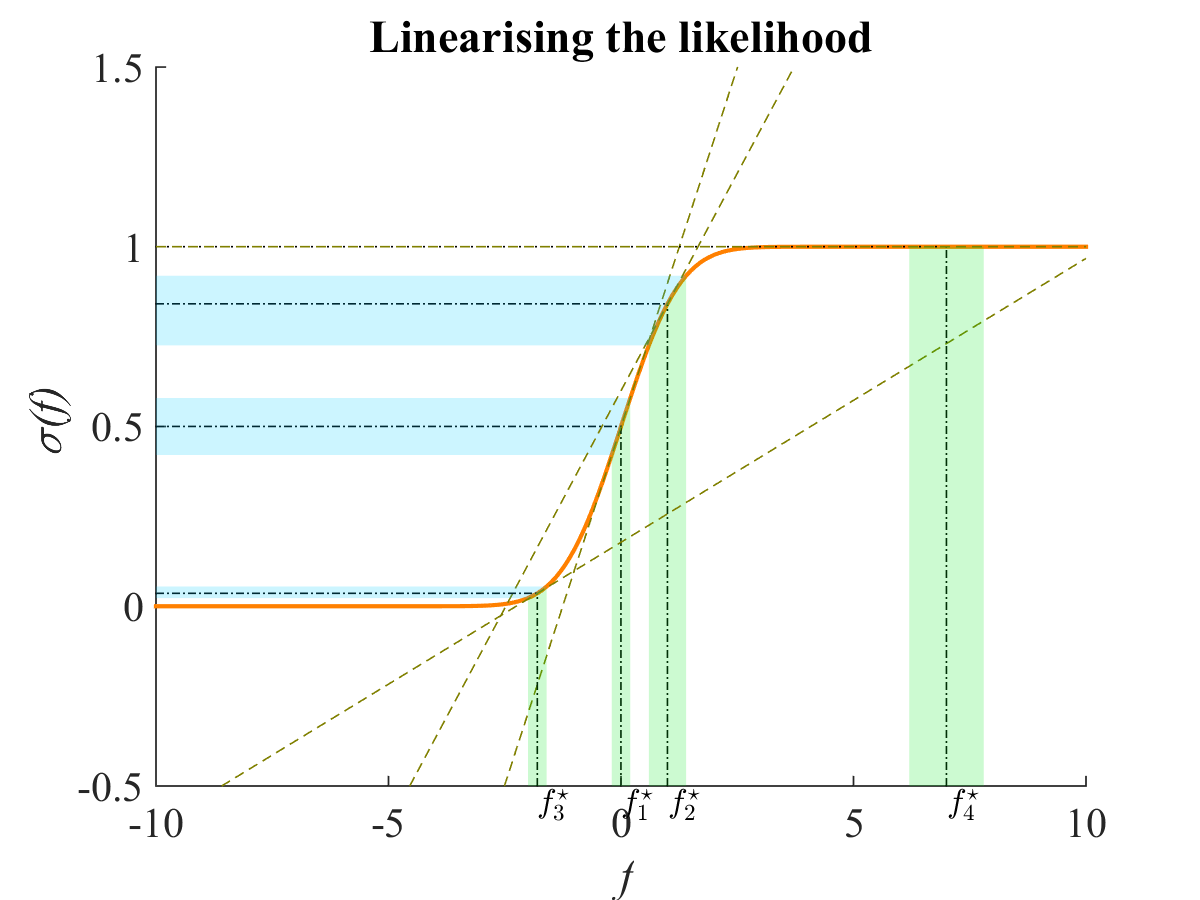
\includegraphics[width = \linewidth]{Figures/linearisation.png}
			\caption{Linearisation accuracy for a probit response: Green shade represents the latent variance while blue shade represents the predictive variance. Gold lines show local linearisation about latent expectance.}
			\label{Figure:Linearisation}
		\end{figure}
			
		As the predictive probabilities are nonlinear transformations of the Gaussian distributed latent vector, they are no longer Gaussian distributed. Hence, we propose linearising the response function about the latent expectance $\bar{f}^{\star}_{i} := \mathbb{E}[f^{\star}_{i}]$. Figure \ref{Figure:Linearisation} illustrates the linearisation accuracy for a probit response. Observe that points with latent expectance far away from zero translate to near zero predictive variance even under high latent variance. Linearisation is thus very accurate for those points. For points with latent expectances near zero, we require the latent variances to be sufficiently small for linearisation to be accurate.

		\begin{figure}[!htbp]
		\centering
			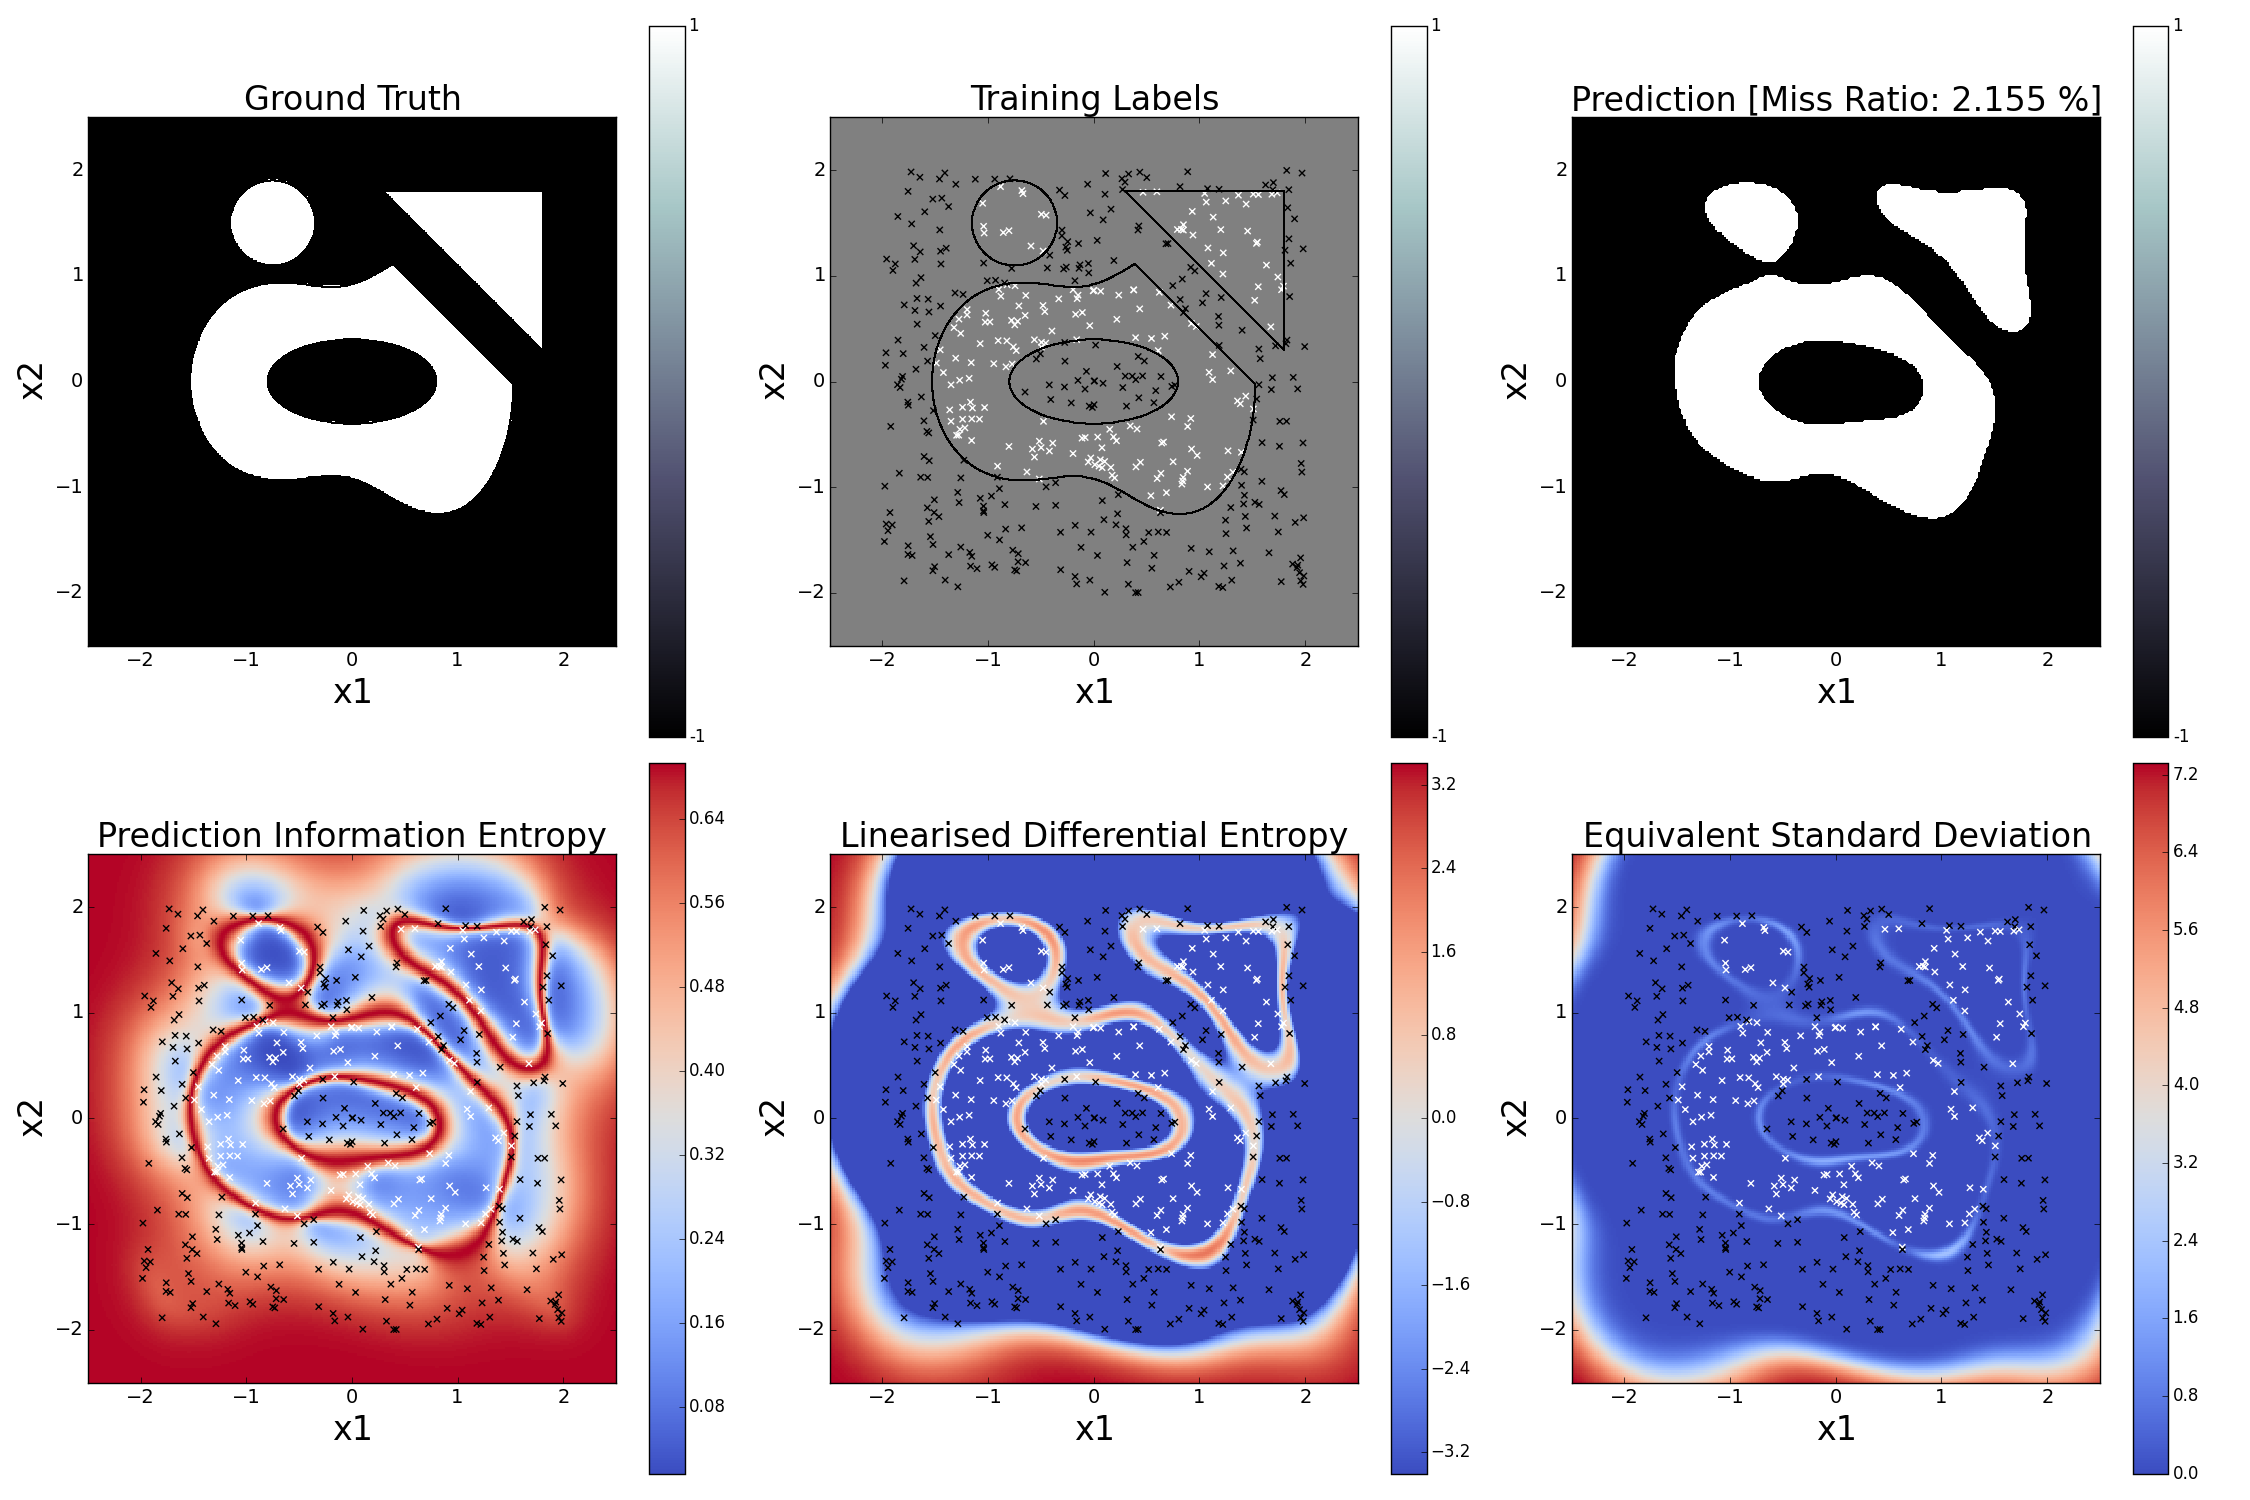
\includegraphics[width = \linewidth]{Figures/binary_linearised_entropy_horizontal/Figure1.png}
		\caption{Binary Classifier Example}
		\label{Figure:Results:BinaryLinearisedEntropy}
		\end{figure}
		
		\subsubsection{Derivation}
		
			We proceed to derive the linearisation which also serves to construct the definition of linearised differential entropy. With first order Taylor expansion, we linearise the response about the chosen linearisation point $\bar{f}^{\star}_{i} = \mathbb{E}[f^{\star}_{i}]$.
			
			\begin{equation}
				\sigma(f^{\star}_{i}) \approx \sigma_{L}(f^{\star}_{i}) := \sigma(\bar{f}^{\star}_{i}) + \sigma'(\bar{f}^{\star}_{i}) (f^{\star}_{i} - \bar{f}^{\star}_{i})
			\label{Section:LinearisedEntropy:Equation:LinearisingSigmoid}
			\end{equation}
			
			The prediction probabilities are now approximated as a linear transformation $\sigma_{L}(f)$ of the latent vector, so that it is also multivariate Gaussian distributed with expectance and covariance available in analytical form \eqref{Section:LinearisedEntropy:Equation:MomentsLinearisedSigmoid}.
			
			\begin{align*}
			\numberthis \label{Section:LinearisedEntropy:Equation:MomentsLinearisedSigmoid}
					\vec{\sigma}_{L}(\vec{f}^{\star}) & \sim \mathcal{N}(\vec{\mu}^{\star}_{L}, \Sigma^{\star}_{L}) \\
					({\mu^{\star}_{L}})_{i} & = \mathbb{E}[\sigma_{L}(f^{\star}_{i})] = \sigma(\bar{f}^{\star}_{i}) \\
					({\Sigma^{\star}_{L}})_{ij} & = \mathbb{C}\mathrm{ov}[\sigma_{L}(f^{\star}_{i}), \sigma_{L}(f^{\star}_{j})] = \sigma'(\bar{f}^{\star}_{i}) \sigma'(\bar{f}^{\star}_{j}) \mathbb{C}\mathrm{ov}[f^{\star}_{i}, f^{\star}_{j}]
			\end{align*}
			
			We then define the linearised differential entropy $H^{\star}_{L}$ at the query points $X^{\star}$ to be the differential entropy for which the random vector $\vec{\sigma}_{L}(\vec{f}^{\star})$ holds. Since $\vec{\sigma}_{L}(\vec{f}^{\star})$ is multivariate Gaussian distributed, $H_{L}$ exhibits a closed form \eqref{Section:LinearisedEntropy:Equation:BinaryLinearisedEntropy}.
			
			\begin{equation}
				H^{\star}_{L} := \frac{1}{2} \log\Big((2 \pi e)^{n^{\star}} \det(\Sigma^{\star}_{L})\Big)
			\label{Section:LinearisedEntropy:Equation:BinaryLinearisedEntropy}
			\end{equation}			
					
	\subsection{Multiclass Classification}
			
		For multiclass classification, linearisation is performed on the softmax function $\sigma^{m}$ which returns the corresponding predictive class probability $\vec{\pi}^{m}$ for class $m$ \eqref{Section:LinearisedEntropy:Equation:Softmax}. For notational clarity we move the query star ($^\star$) to the left and use the superscript $m$ to index the classes. The latent vector $\vec{f}_{i} := \{f^{m}_{i}\}_{m \in \{1, 2, \dots, c\}}$ represents the collection of $c$ latent values across classes at the query point $i$, and is distinct from $\vec{f}^{m} := \{f^{m}_{i}\}_{i \in \{1, 2, \dots, n^{\star}\}}$ which represents the collection of $n^{\star}$ latent values across query points for class $m$.

		\begin{equation}
			^{\star}\pi^{m}_{i} = \sigma^{m}(^{\star}\vec{f}_{i}) := \frac{\exp(^{\star}f^{m}_{i})}{\sum_{l = 1}^{c} \exp(^{\star}f^{l}_{i})} \qquad m \in \{1, 2, \dots, c\}
		\label{Section:LinearisedEntropy:Equation:Softmax}
		\end{equation}
			
		\begin{figure}[!htbp]
		\centering
			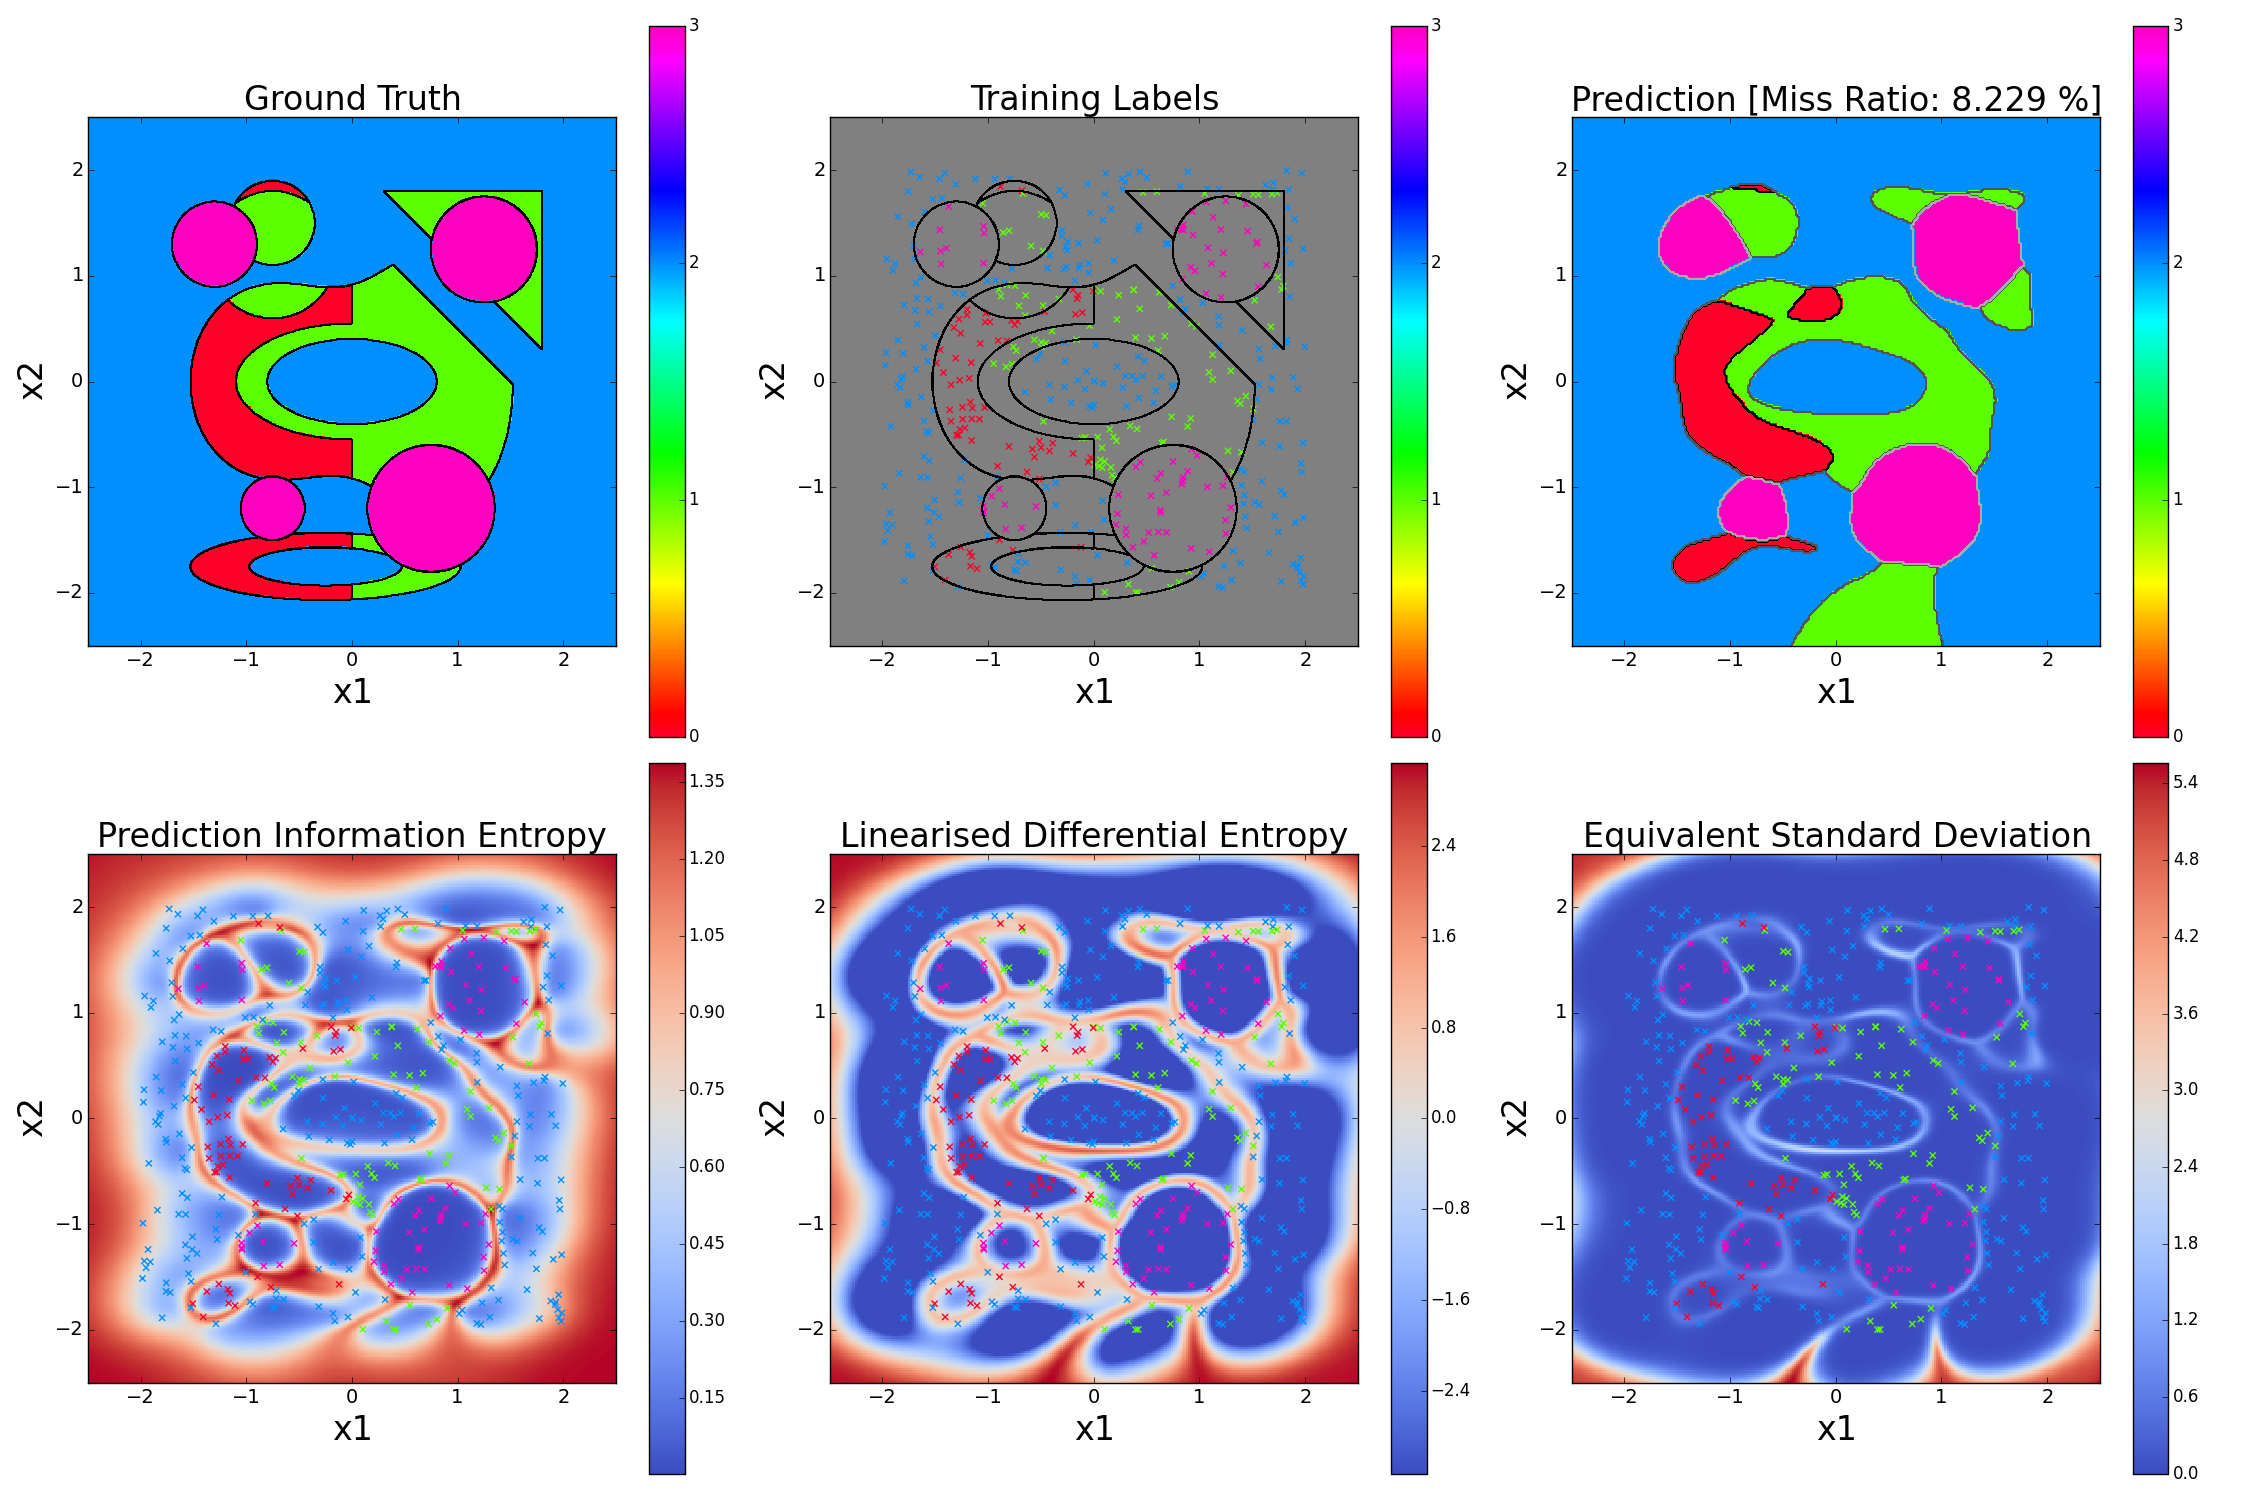
\includegraphics[width = \linewidth]{Figures/multiclass_linearised_entropy_horizontal/Figure1.png}
		\caption{Multiclass Classifier Example}
		\label{Figure:Results:MulticlassLinearisedEntropy}
		\end{figure}
		
		\subsubsection{Derivation}
		
			Similar to the binary case, to linearise we first find the gradient of each of the $c$ softmax functions \eqref{Section:LinearisedEntropy:Equation:SoftmaxGradient}. For notational simplicity, the query stars ($^{\star}$) are omitted in this derivation.
			
			\begin{equation}
				\frac{\partial \sigma^{m}}{\partial f^{k}_{i}}(\vec{f}_{i}) =
				\begin{cases} 
					- \frac{\exp(f^{m}_{i}) \exp(f^{k}_{i})}{\sum_{l = 1}^{c} \exp(f^{l}_{i})} & \text{for } k \neq m  \\
					- \frac{\exp(f^{m}_{i})^{2}}{\big(\sum_{l = 1}^{c} \exp(f^{l}_{i})\big)^{2}} + \frac{\exp(f^{m}_{i})}{\sum_{l = 1}^{c} \exp(f^{l}_{i})}& \text{for } k = m
				\end{cases}
			\label{Section:LinearisedEntropy:Equation:SoftmaxGradient}
			\end{equation}			
		
			The numerators are explicitly left in the products of exponentiation instead of exponentiation of sums to reflect ways to cache quantities during computation. 
			
			Hence, for each class $m$ at query point $i$ we have compute a softmax gradient vector \eqref{Section:LinearisedEntropy:Equation:SoftmaxGradientVector}.
			
			\begin{equation}
				\frac{\partial \sigma^{m}}{\partial \vec{f}_{i}}(\vec{f}_{i}) := \begin{bmatrix} \frac{\partial \sigma^{m}}{\partial f^{1}_{i}}(\vec{f}_{i}) & \frac{\partial \sigma^{m}}{\partial f^{2}_{i}}(\vec{f}_{i}) & \dots & \frac{\partial \sigma^{m}}{\partial f^{c}_{i}}(\vec{f}_{i}) \end{bmatrix}^{T}
			\label{Section:LinearisedEntropy:Equation:SoftmaxGradientVector}
			\end{equation}
			
			The linearisation is again performed on the mean latent predictions $\bar{\vec{f}}_{i} = \mathbb{E}[\vec{f}_{i}]$ so that the we can approximate the softmax $\sigma^{m}(\vec{f}_{i})$ with the linearised softmax $\sigma^{m}_{L}(\vec{f}_{i})$ \eqref{Section:LinearisedEntropy:Equation:LinearisedSoftmax} in an analogous form as \eqref{Section:LinearisedEntropy:Equation:LinearisingSigmoid}.
			
			\begin{equation}
				\begin{aligned}
					\sigma^{m}(\vec{f}_{i}) \approx \sigma^{m}_{L}(\vec{f}_{i}) & := \sigma^{m}(\bar{\vec{f}}_{i}) + \left. \frac{\partial \sigma^{m}}{\partial \vec{f}_{i}} \right|^{T}_{\vec{f}_{i} = \bar{\vec{f}}_{i}} (\vec{f}_{i} - \bar{\vec{f}}_{i}) \\
					& = \vec{c}^{m}_{i} + (\vec{g}^{m}_{i})^{T} (\vec{f}_{i} - \bar{\vec{f}}_{i})
				\end{aligned}
			\label{Section:LinearisedEntropy:Equation:LinearisedSoftmax}
			\end{equation}
			
			where we have notated the constants $\vec{c}^{m}_{i} := \sigma^{m}(\bar{\vec{f}}_{i})$ and $\vec{g}^{m}_{i} := \frac{\partial \sigma^{m}}{\partial \vec{f}_{i}}(\bar{\vec{f}}_{i})$.
			
			To determine the distribution of the vector of softmax values across query points, we first define the following \eqref{Section:LinearisedEntropy:Equation:Definitions}.
			
			\begin{equation}
				\begin{aligned}
					F &:= \{f^{m}_{i}\}_{m \in \{1, 2, \dots, c\}, i \in \{1, 2, \dots, n^{\star}\}} \in \mathbb{R}^{c \times n^{\star}} \\
					\vec{\sigma}^{m}_{L}(F) &:= \begin{bmatrix} \sigma^{m}_{L}(\vec{f}_{1}) & \sigma^{m}_{L}(\vec{f}_{2}) & \dots & \sigma^{m}_{L}(\vec{f}_{n^{\star}}) \end{bmatrix}^{T}
				\end{aligned}
			\label{Section:LinearisedEntropy:Equation:Definitions}
			\end{equation}
						
			We can now compute compute the covariance of the linearised sigmoid of a particular class $m$ between two query points $i$ and $j$, as well as the expectance at a particular query point $i$ \eqref{Section:LinearisedEntropy:Equation:MomentsLinearisedSoftmax}.
			
			\begin{align*}
			\numberthis \label{Section:LinearisedEntropy:Equation:MomentsLinearisedSoftmax}
					\vec{\sigma}^{m}_{L}(F) & \sim \mathcal{N}(\vec{\mu}^{m}_{L}, \Sigma^{m}_{L}) \\
					(\mu^{m}_{L})_{i} & = \mathbb{E}[\sigma^{m}_{L}(\vec{f}_{i})] =  \sigma^{m}(\bar{\vec{f}}_{i}) \\
					(\Sigma^{m}_{L})_{ij} & = \mathbb{C}\mathrm{ov}[\sigma^{m}_{L}(\vec{f}_{i}), \sigma^{m}_{L}(\vec{f}_{i})] \\
					& = \mathbb{C}\mathrm{ov}[(\vec{g}^{m}_{i})^{T} \vec{f}_{i}, (\vec{g}^{m}_{j})^{T} \vec{f}_{j}] \\
					& = \sum_{k = 1}^{c} (g^{m}_{i})^{k} (g^{m}_{j})^{k} \mathbb{C}\mathrm{ov}[f^{k}_{i}, f^{k}_{j}]
			\end{align*}
						
			where $(g^{m}_{i})^{k}$ denotes the $k^{\text{th}}$ element of $\vec{g}^{m}_{i}$. The last equality arises as a result of employing the OVA multiclass classification, where latent values of class $i$ and class $j$ are conditionally independent given training observations.
			
			Finally, we define the linearised entropy of the OVA multiclass Gaussian process classifier as follows \eqref{Section:LinearisedEntropy:Equation:MulticlassLinearisedEntropy}.
			
			\begin{equation}
				H_{L} := \frac{1}{2} \log\Bigg((2 \pi e)^{n^{\star}} \det\bigg(\sum_{m = 1}^{c} \Sigma^{m}_{L}\bigg)\Bigg)
			\label{Section:LinearisedEntropy:Equation:MulticlassLinearisedEntropy}
			\end{equation}			
	
\section{Receding Horizon Approach to Informative Path Planning}
\label{Section:RecedingHorizonApproach}

	In this section we present a receding horizon approach to the informative path planning problem. Specifically, we use the differential linearised entropy derived earlier as the acquisition function. We motivate the use of the approach and discuss its properties. Performance is then assessed with the Scott Reef dataset.
	
	\subsection{Motivation}
	
		The receding horizon approach is inspired by the philosophy of model predictive control (MPC) in control theory, for which a continuous problem is discretised and an optimal control problem is transcribed into a static optimisation problem at each time step. Similar to MPC, while receding horizon methods are almost always suboptimal, it provides a computationally tractable approach that is rather stable in performance. Furthermore, a receding horizon approach avoids a myopic, or greedy, approach to informative path planning. Myopic approaches often result in the vehicle fixating on a region with local maximum entropy due to its inability to sacrifice immediate gain for future gains in a faraway region. Lastly, a receding horizon approach is simple to implement and sufficient for most missions for which, instead of optimality, only stability of information gain is desired. 
		
		Informative path planning is a highly dynamical process in which the observations the vehicle decides to take can significantly impact the belief space of the vehicle and hence alter its action. As a result, Gaussian processes are often used for modeling the environment for which path planning is to be performed. The tractability of Gaussian processes regression allows sophisticated methods for informative path planning, such as  performing sequential Bayesian optimisation to achieve informative path planning over continuous domains \cite{SequentialBayesianOptimisation}. One desired property we would like to achieve with an informative path planning problem is that the search is non-myopic. When the objective is to collect data on a particular spatial phenomenon, Gaussian process regression can be used as the model under which strong theoretical performance guarantees can be made \cite{Meliou:2007:NIP:1619645.1619742}. However, in the case where the objective is to collect data in the form of discrete labels, a Gaussian process classifier is used instead for modeling the phenomenon. As discussed earlier, the joint entropy from a Gaussian process classifier is not available in closed form. Instead, another measure of joint entropy was developed in the previous section which demonstrated desired properties for informative exploration. To take advantage of the tractability of linearised differential entropy over finite collections of query points, we discretise the spatial domain and select paths composed of finitely many query points. The acquisition criterion is then set to be the linearised differential entropy of the query points that compose the path.

		
	\subsection{Outline of Method}

		The receding horizon approach requires the selection of a horizon length and the number of control points (query points) for which the path is to be defined upon. The horizon length plays a significant role in the performance of the method. A short horizon length tends to produce path that are similar to a myopic approach. A horizon length that is too long, however, can be both inefficient and destabilising. For an informative path planning scenario, looking ahead too far can have diminishing returns in its informativeness, as the vehicle's belief space would be significantly altered by the time it was supposed to follow the original proposed path. The horizon length selected for the Scott Reef data is 5 km with 30 control points.
		
		Figure \ref{Figure:Results:RecedingHorizonMethodOutline} describes the basic flow of approach, which resembles the approach of MPC in control theory. The acquisition function to be maximised in each step is the linearised differential entropy \eqref{Section:LinearisedEntropy:Equation:MulticlassLinearisedEntropy}. A new path is proposed in each step for which the vehicle only executes the policy for towards the first control point, takes an observation, relearn the GP classifier model, and repeats the process. 
		
		\begin{figure}[!htbp]
		\centering
			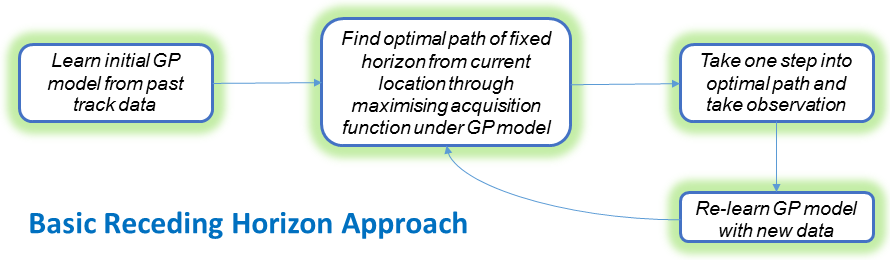
\includegraphics[width = \linewidth]{Figures/receding_horizon_informative_path_planning.png}
		\caption{Basic Receding Horizon Structure}
		\label{Figure:Results:RecedingHorizonMethodOutline}
		\end{figure}
		
\section{Discussion}

	\subsection{Interpretation of Linearised differential entropy}
	
		It is worthwhile to remember that linearised differential entropy is not an approximation to the usual prediction information entropy - the former is a differential entropy on a multivariate Gaussian distribution and the later is an information entropy on the distribution of discrete class predictions combinations. They have different interpretations and both have advantageous properties under different settings. We propose using linearised differential entropy as an alternative acquisition function for informative path planning which can be more beneficial under specific exploration purposes.
		
		Here we compare the linearised differential entropy with the usual prediction information entropy of the Gaussian process classifier. For visualisation purposes, only the marginalised entropies are shown. We show examples where abundant information is available, where the difference in the properties in the two measures can be emphasized. 
		
		Figure \ref{Figure:Results:BinaryLinearisedEntropy} show a simple binary classification problem with abundant data on features $x_{1}$ and $x_{2}$, allowing a misclassification rate of 2.155\%. The classifier is trained with an axis aligned Gaussian kernel with a probit response under Laplace approximation. 

		In this example, there are no training points around the edges shown. As a result, the GP classifier learns a slightly lower signal to noise ratio in the latent function, and bounces back to its latent GP prior for which it remains uncertain regarding class label assignments. The prediction information entropy reflects this change more rapidly, so that it is high both at the decision boundaries and wherever observations are lacking. If the acquisition function for informative exploration is a function of the prediction information entropy, the vehicle would be suggested to explore both places with lacking observations and the decision boundaries. 
		
		On the other hand, linearised differential entropy focuses on the decision boundary as it is constructed to be only high when the latent function is near zero \ref{Figure:Linearisation}. We can see in figure \ref{Figure:Results:BinaryLinearisedEntropy} that the linearised differential entropy emphasizes on where the latent expectance is close to zero, and filters out the rest. If the linearised differential entropy is used as the acquisition function, the vehicle would focus on the decision boundaries within the feature space. Notice that regions far away from observations in the feature space are also assigned with high linearised differential entropy, as the latent function bounces back to its prior, so that the vehicle would explore those parts of the feature space if necessary.
		
%		Intuitively, under abundant data, we would like the classifier to only indicate high entropies at decision boundaries. In figure \ref{Figure:Results:BinaryLinearisedEntropy}, we see that the prediction information entropy is indeed near its maximum at the predict decision boundaries. As an artefact of the Laplace approximation, however, it is also quite high around the edges where the classifier has learned a slightly lower signal to noise ratio. As there are no data points around the edges, the GP classifier learns a latent function that bounces back to its latent GP prior for which it remains uncertain regarding the class labels. 
		
%		This suggests that if the prediction information entropy is used as the acquisition function for path planning, the vehicle would be suggested to spent some time travelling around the region of interest, collecting data it is already expecting. The prediction entropy is high at both predicted decision boundaries and also places with lower relative data density compared. 
%		
%		This leads to the classic exploration-exploitation dilemma most machine learning algorithms face. It is possible that there exists decision boundaries yet to be detected at regions of lower relative data density. Is it worth it for the vehicle to explore and discover such regions, or exploit the currently known boundaries and map it better? In most exploration applications, the priority is to map the region of interest as accurately and fast as possible in order to reduce time and cost. While it is possible that there exists undiscovered decision boundaries at regions of lower relative data density, it is undesirable under cost constraints that this possibility is weighed heavily by the vehicle even under abundant data.
		
		This demonstrates the advantage of linearised differential entropy. We can see in figure \ref{Figure:Results:BinaryLinearisedEntropy} that the linearised differential entropy is only high at the predicted decision boundaries. Note that the colour scale has been centred around zero differential entropy. Under such an acquisition function, the vehicle would focus strictly on the mapping the predicted decision boundaries better.
		
		Figure \ref{Figure:Results:MulticlassLinearisedEntropy} shows a similar scenario with a multi-class scenario with 4 labels. This classifier is trained through an one v.s. all approach with 4 binary classifiers using the same setup described above. Clearly the same behaviour as the binary case is observed, where the linearised differential entropy approach pushes down the entropy level of all regions except the predicted decision boundaries.
		
		In the case of a feature space that does not contain the spatial coordinates for which path planning in based on, the Monte Carlo Joint Information Entropy Method may spent a lot of time in a single region where it is locally rich in span of a subspace of the feature space. However, this is suboptimal as this means it is giving up on trying to go for other regions that may have an even richer span of the feature space. The linearised differential entropy method focuses its efforts (prioritises) the decision boundaries in the feature space at the expense of overlooking regions with less observations. This leads to smoother paths as it will look at all elements of the feature space. As long as one of the features is spatially correlated (depth in our case), this will lead to smoother paths.
		
\section{Experiment}


	\begin{figure*}[!htbp]
	\centering
		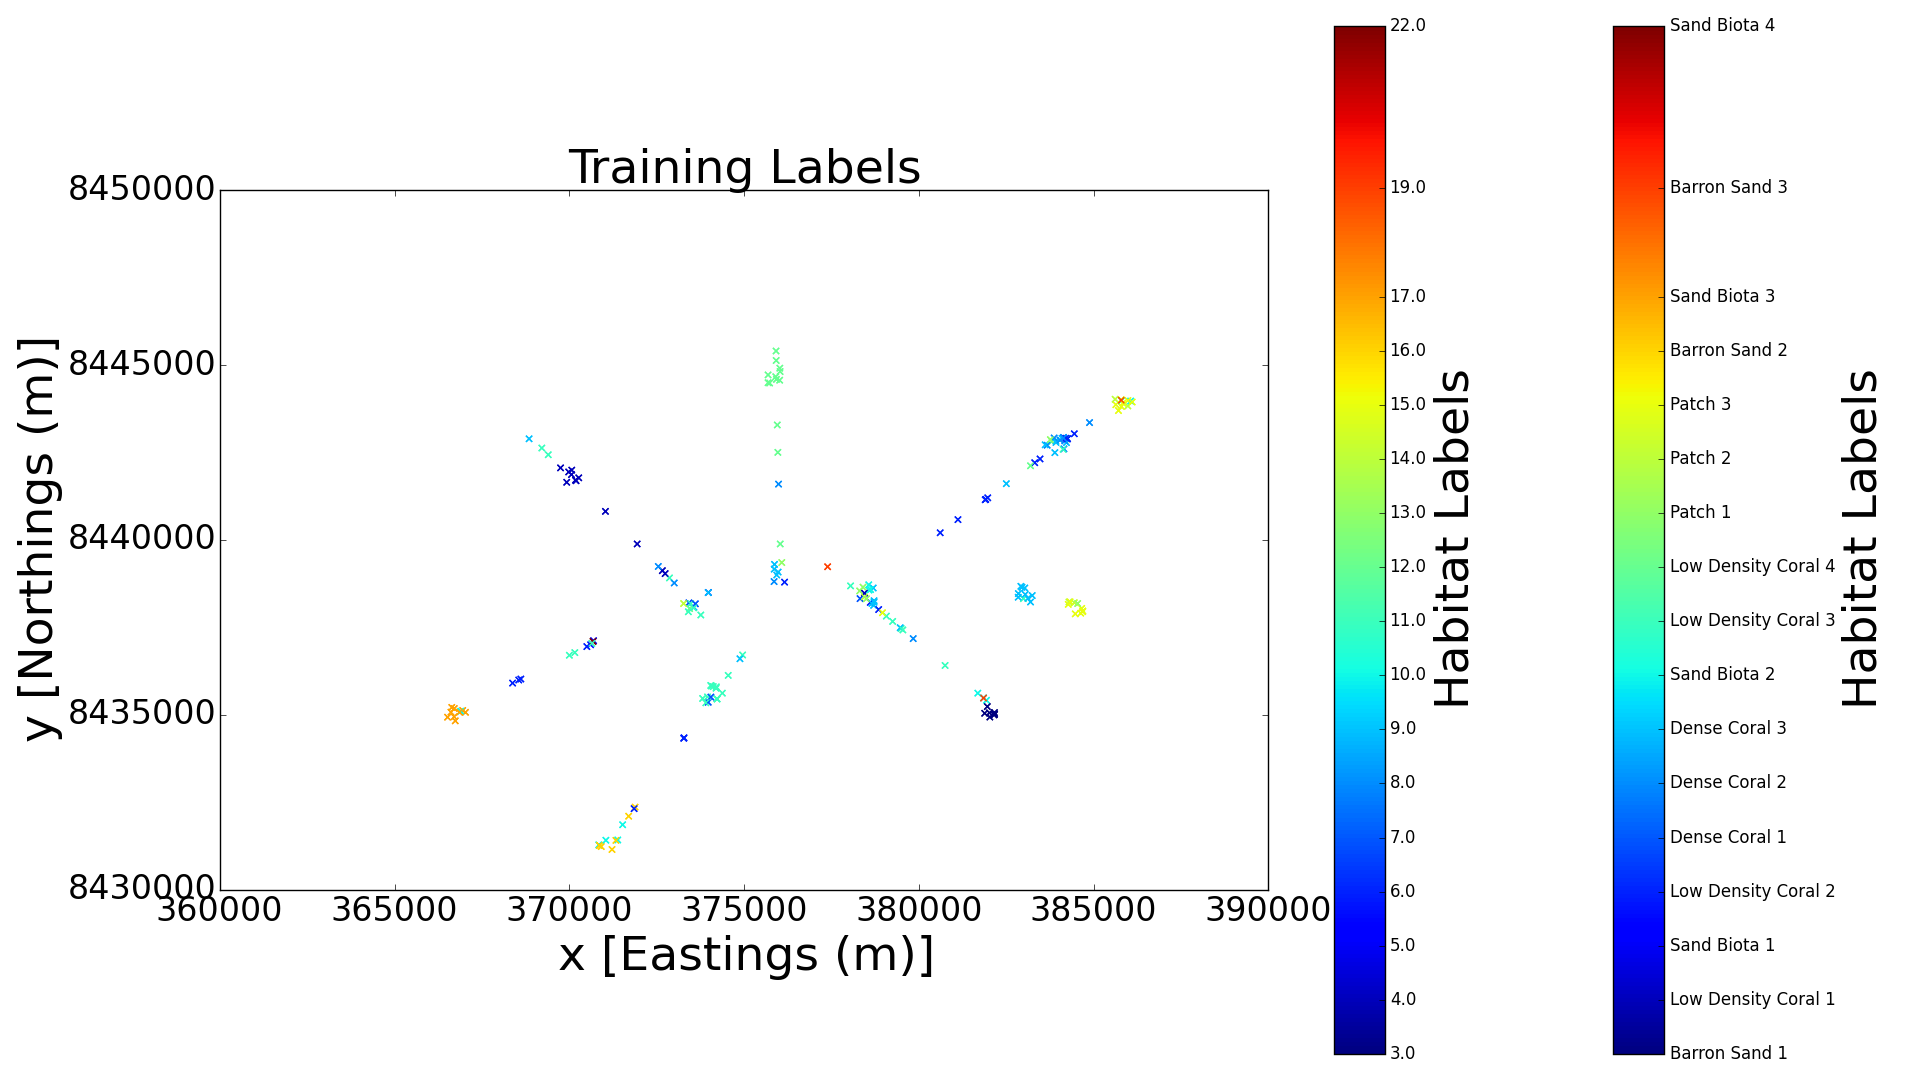
\includegraphics[width = 0.32\linewidth]{Figures/scott_reef_modeling/Figure1.png}
		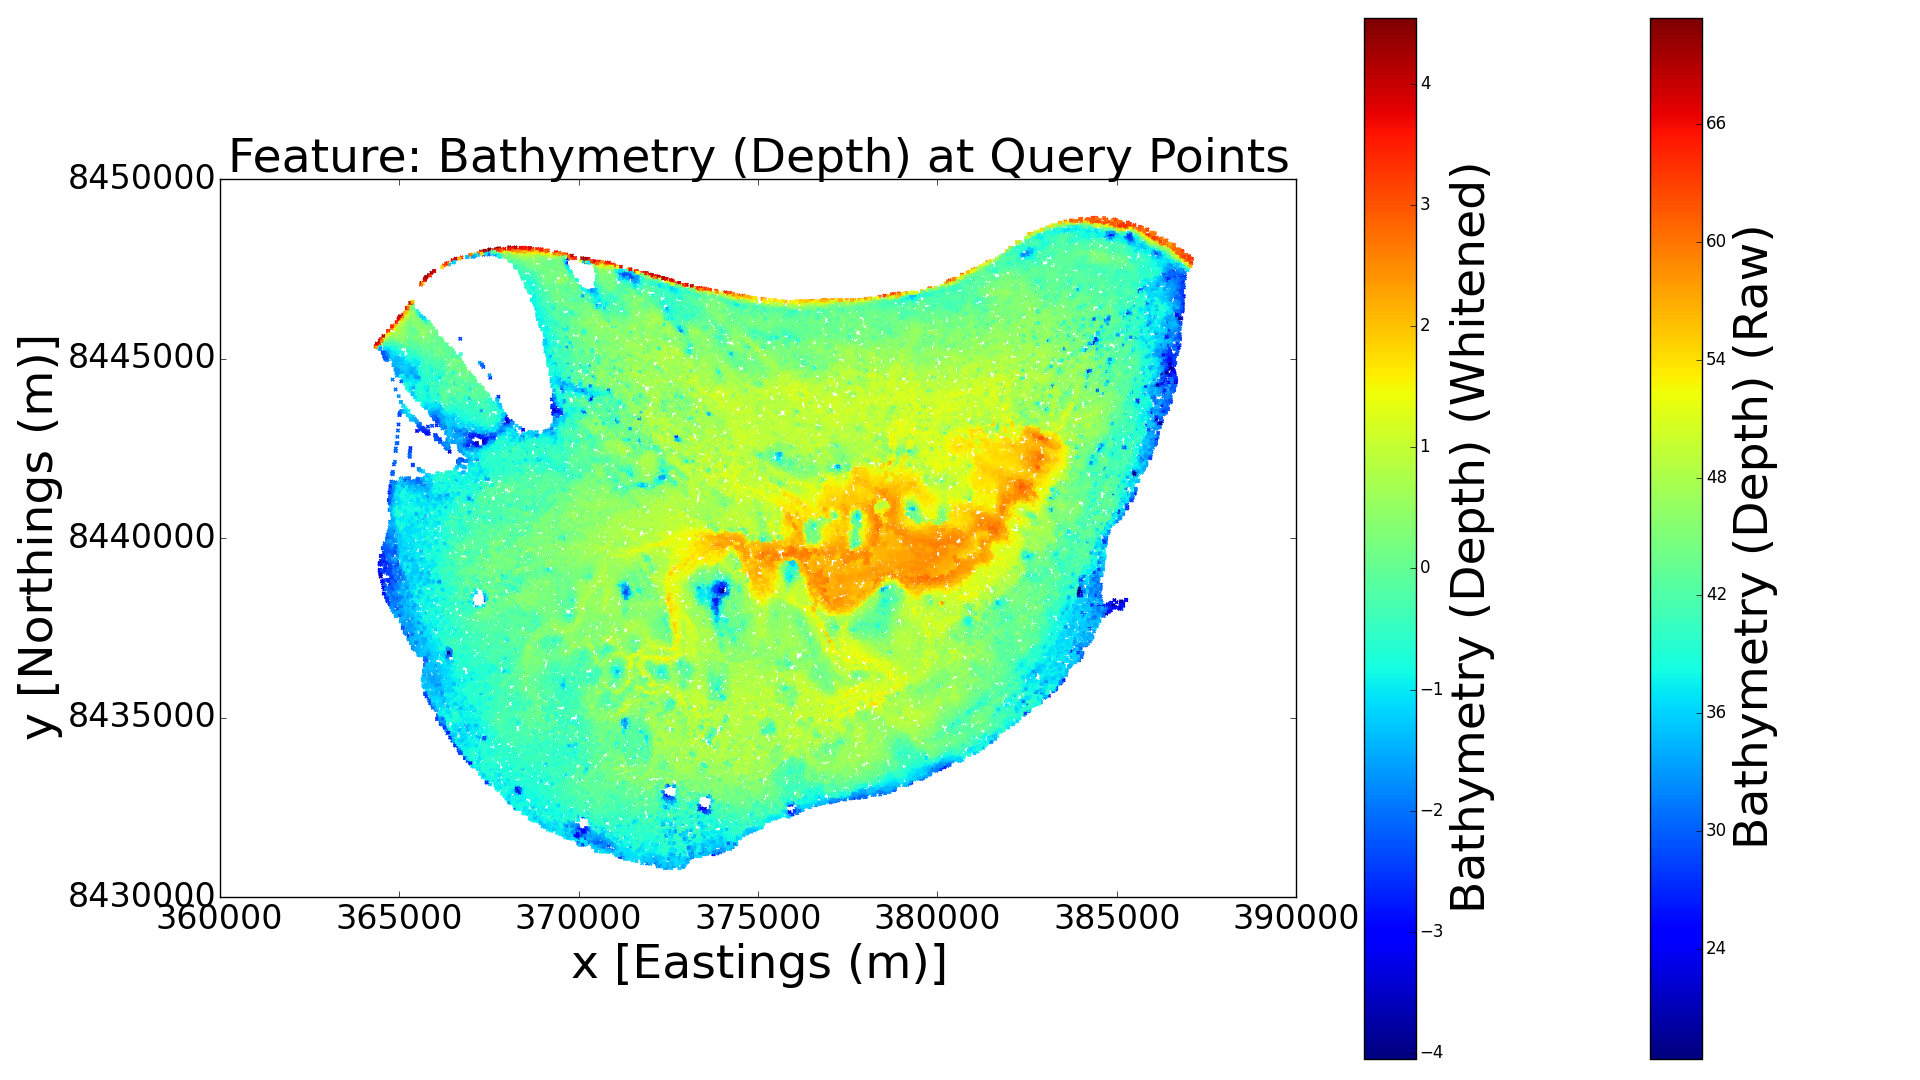
\includegraphics[width = 0.32\linewidth]{Figures/scott_reef_modeling/Figure2.png}
		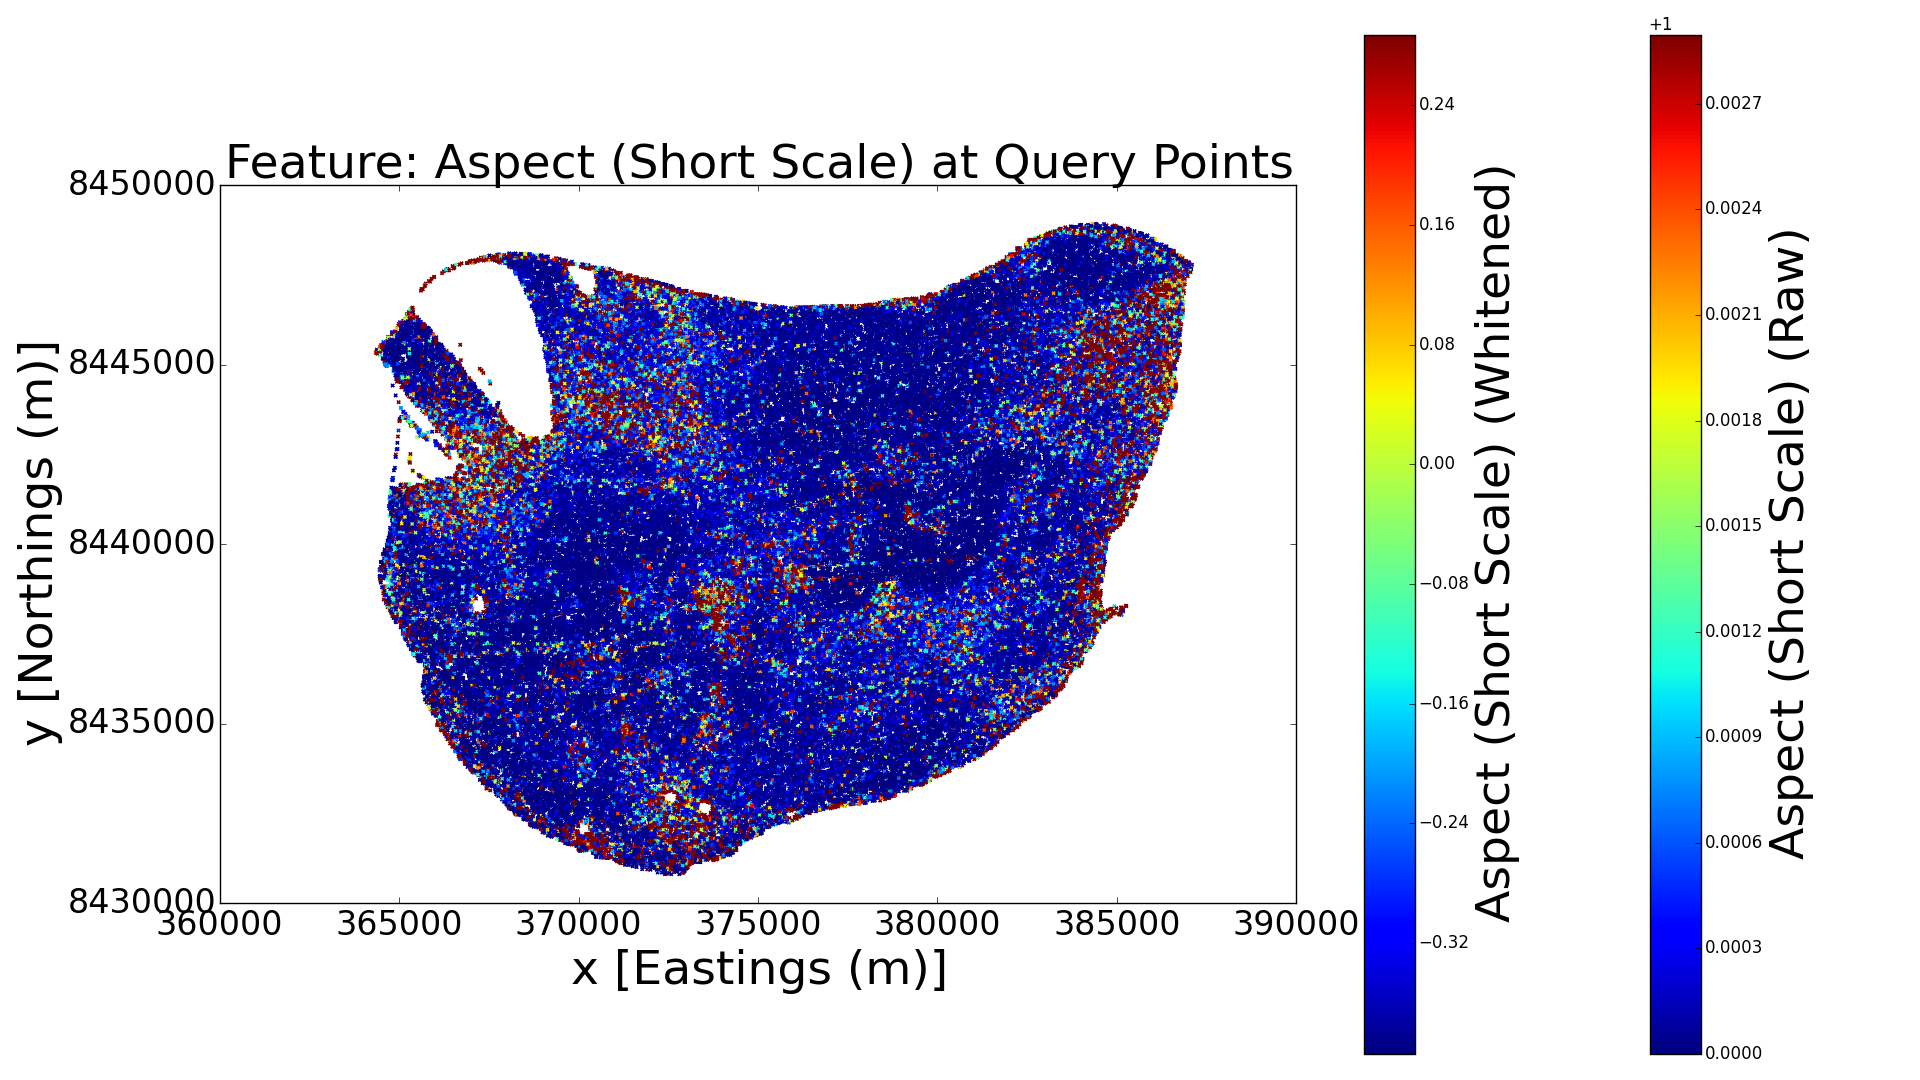
\includegraphics[width = 0.32\linewidth]{Figures/scott_reef_modeling/Figure3.png}
		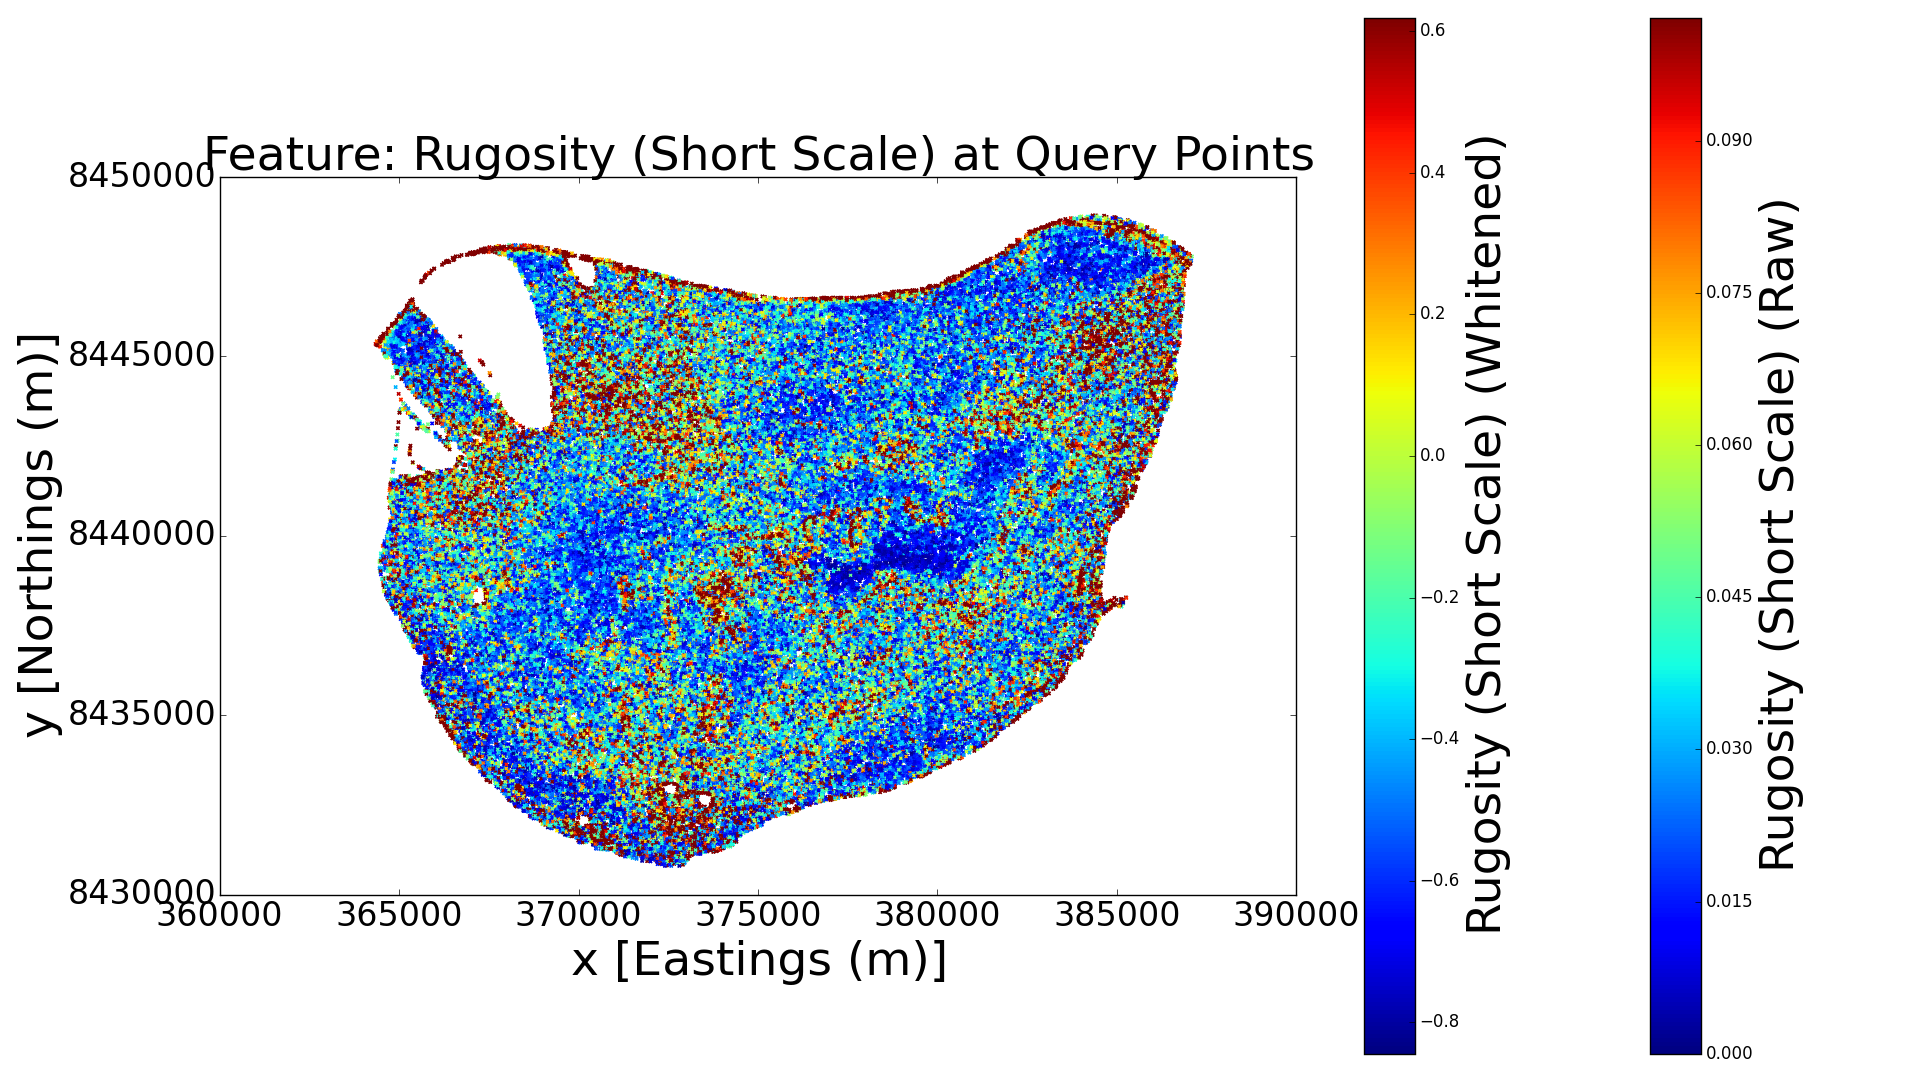
\includegraphics[width = 0.32\linewidth]{Figures/scott_reef_modeling/Figure4.png}
		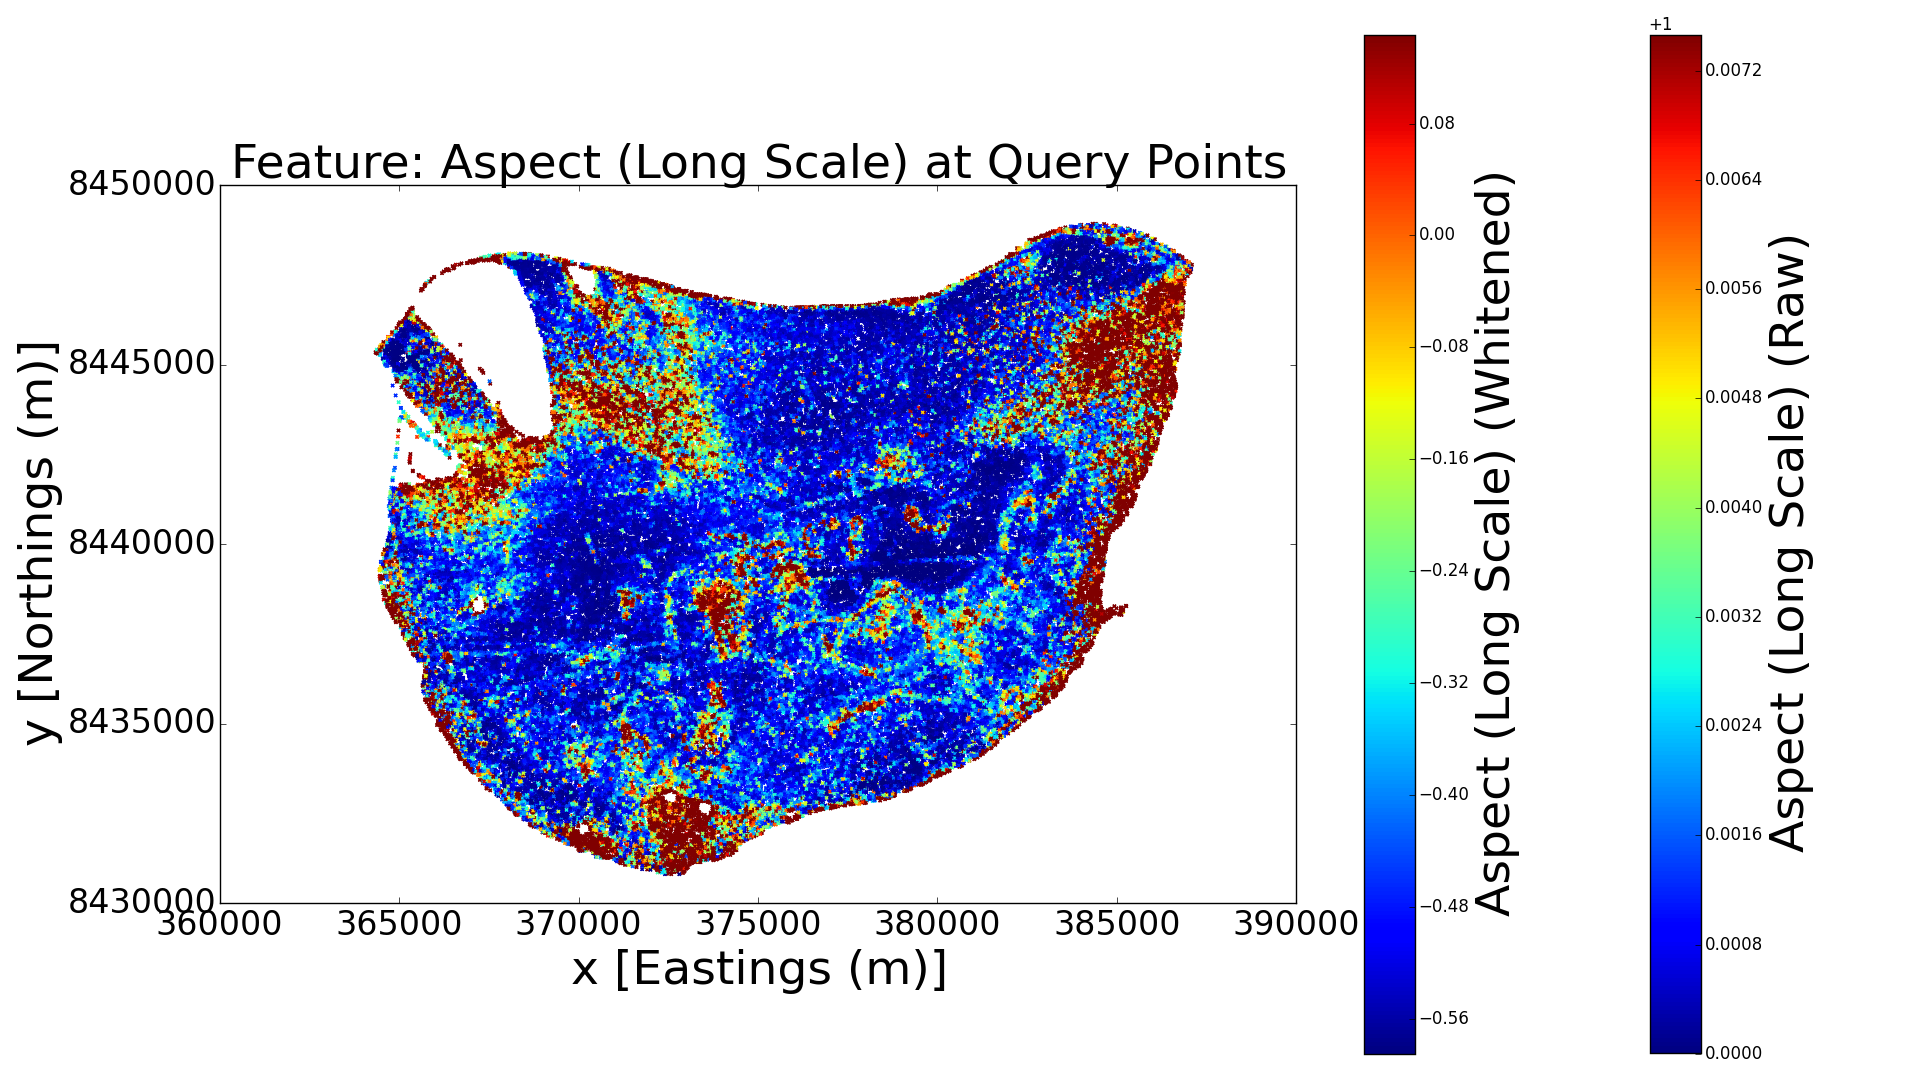
\includegraphics[width = 0.32\linewidth]{Figures/scott_reef_modeling/Figure5.png}
		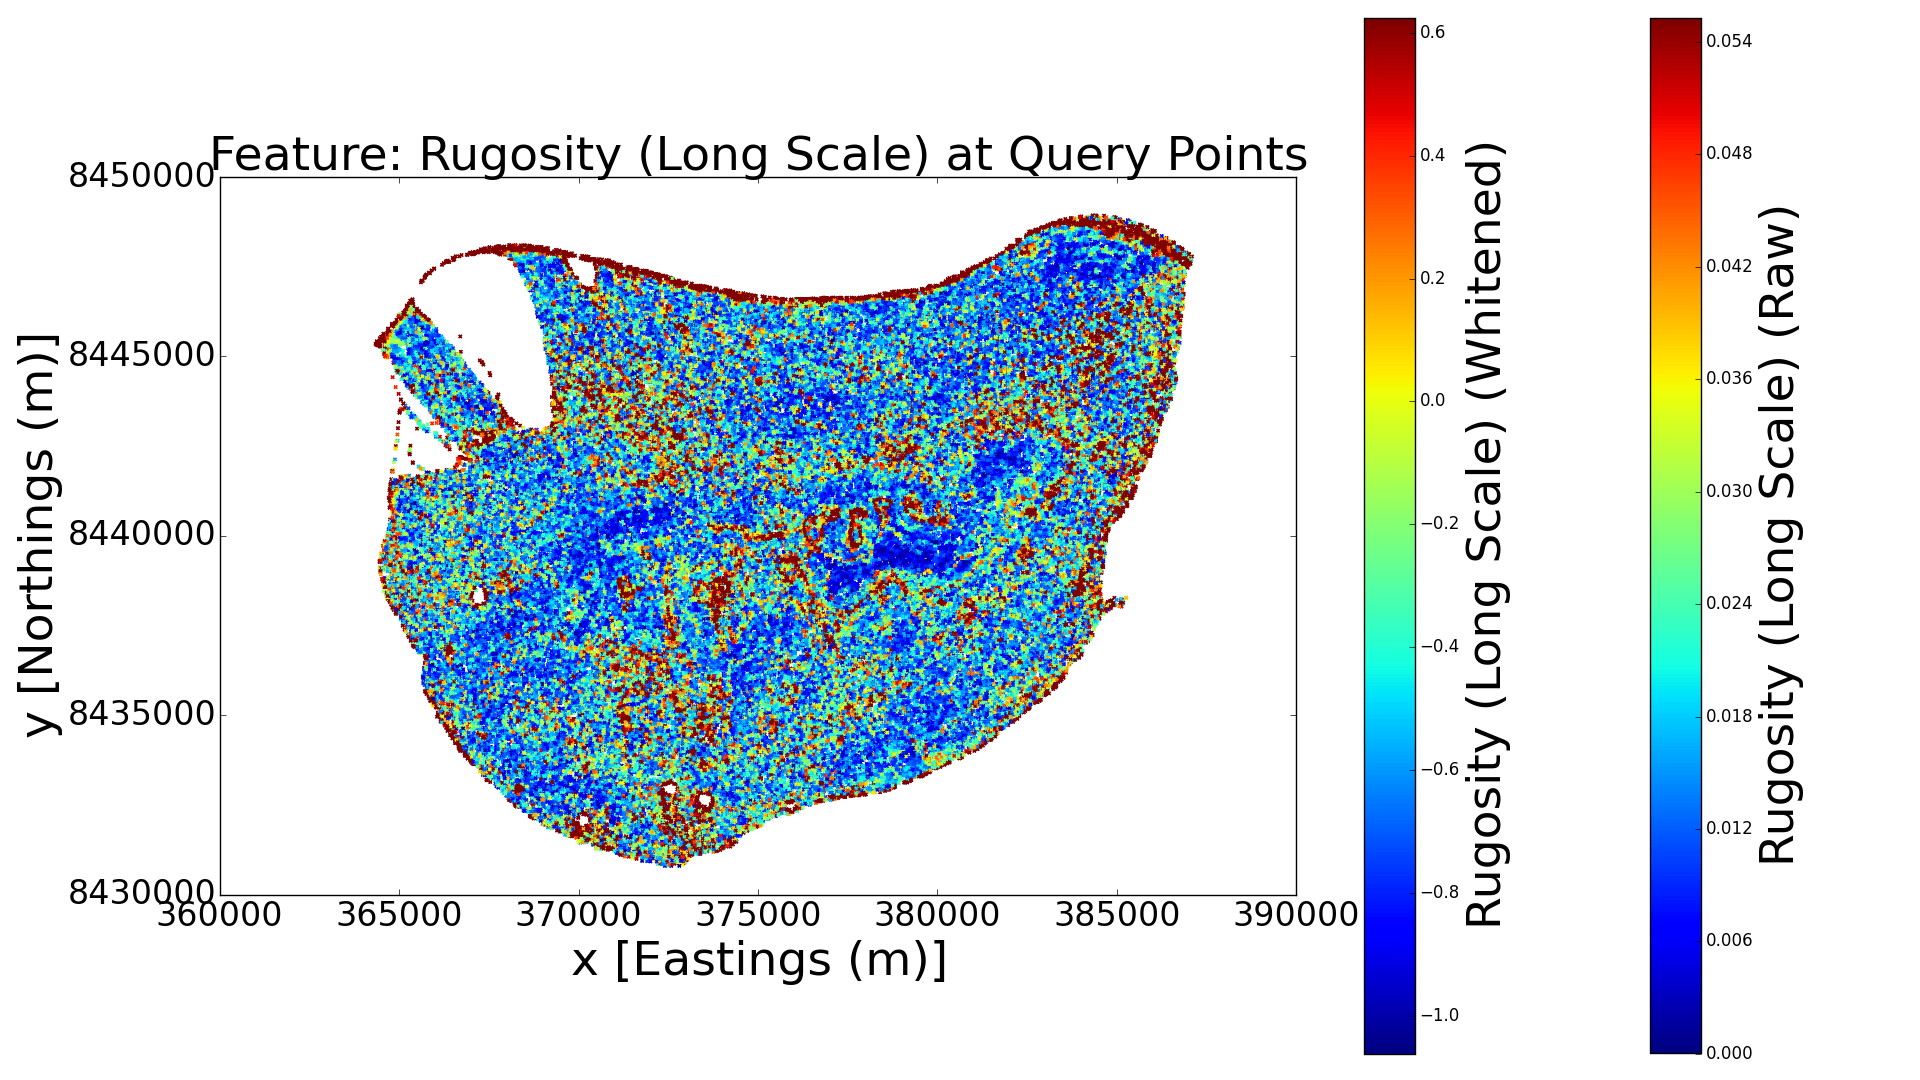
\includegraphics[width = 0.32\linewidth]{Figures/scott_reef_modeling/Figure6.png}
	\caption{Scott Reef Bathymetric Features}
	\label{Figure:Results:ScottReefBathymetricFeatures}
	\end{figure*}


	\subsection{Modeling Scott Reef Benthic Zones}
	
		\begin{figure}[!htbp]
		\centering
			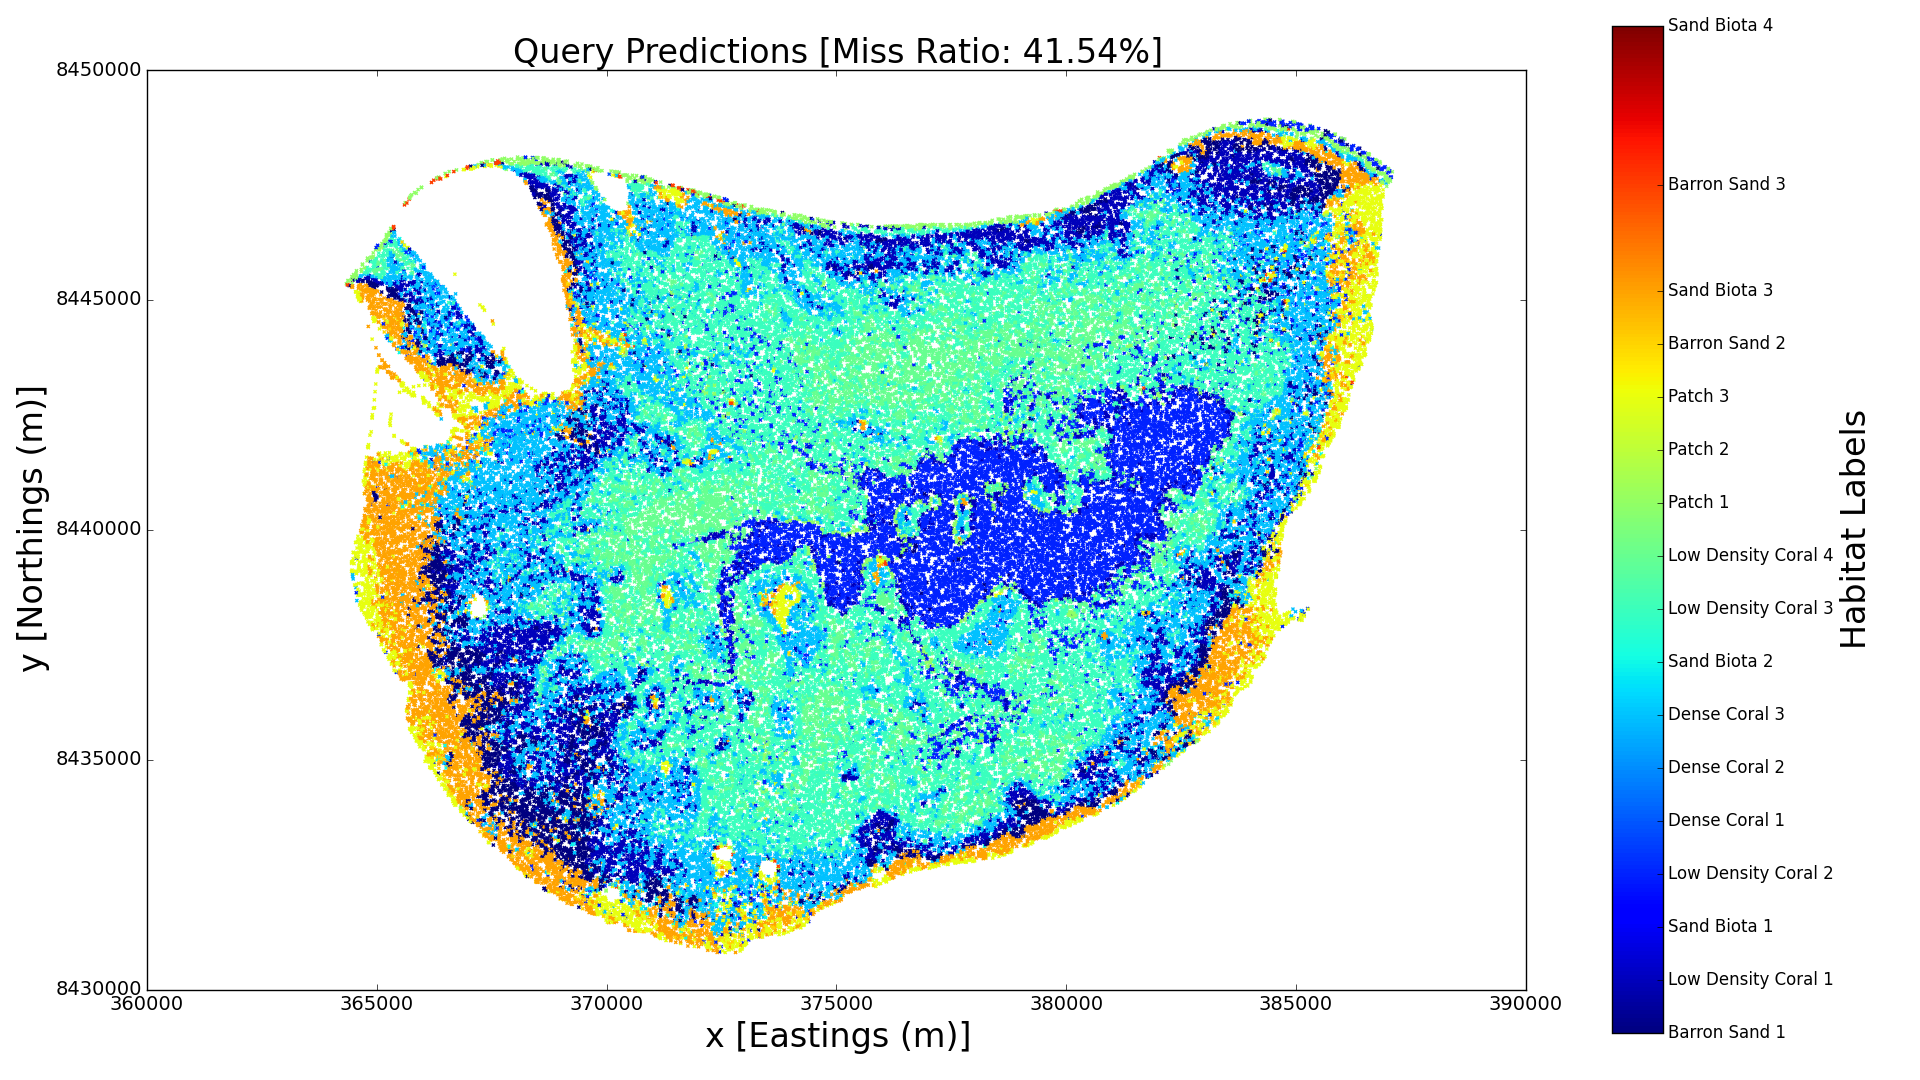
\includegraphics[width = \linewidth]{Figures/scott_reef_modeling/Figure8.png}
		\caption{Scott Reef: Initial Prediction}
		\label{Figure:Results:ScottReefInitialPredictions}
		\end{figure}
		
		The difference between the two measures of entropy is further reinforced when the feature space is distinct from the spatial space for which path planning is to be performed. For our Scott reef example, notice from figure \ref{Figure:Results:ScottReefBathymetricFeatures} that training data is scarce and covers a very limited portion of the feature space. While we can map the reef with an accuracy of 58.46\% using only 200 training points (figure \ref{Figure:Results:ScottReefInitialPredictions}), the prediction information entropy is rather quite high everywhere (figure \ref{Figure:Results:ScottReefPredictionInformationEntropy}). In this initial scenario, under the prediction information entropy criterion the vehicle would simply try to map out all regions as much as possible - a very costly policy.
		
		\begin{figure}[!htbp]
		\centering
			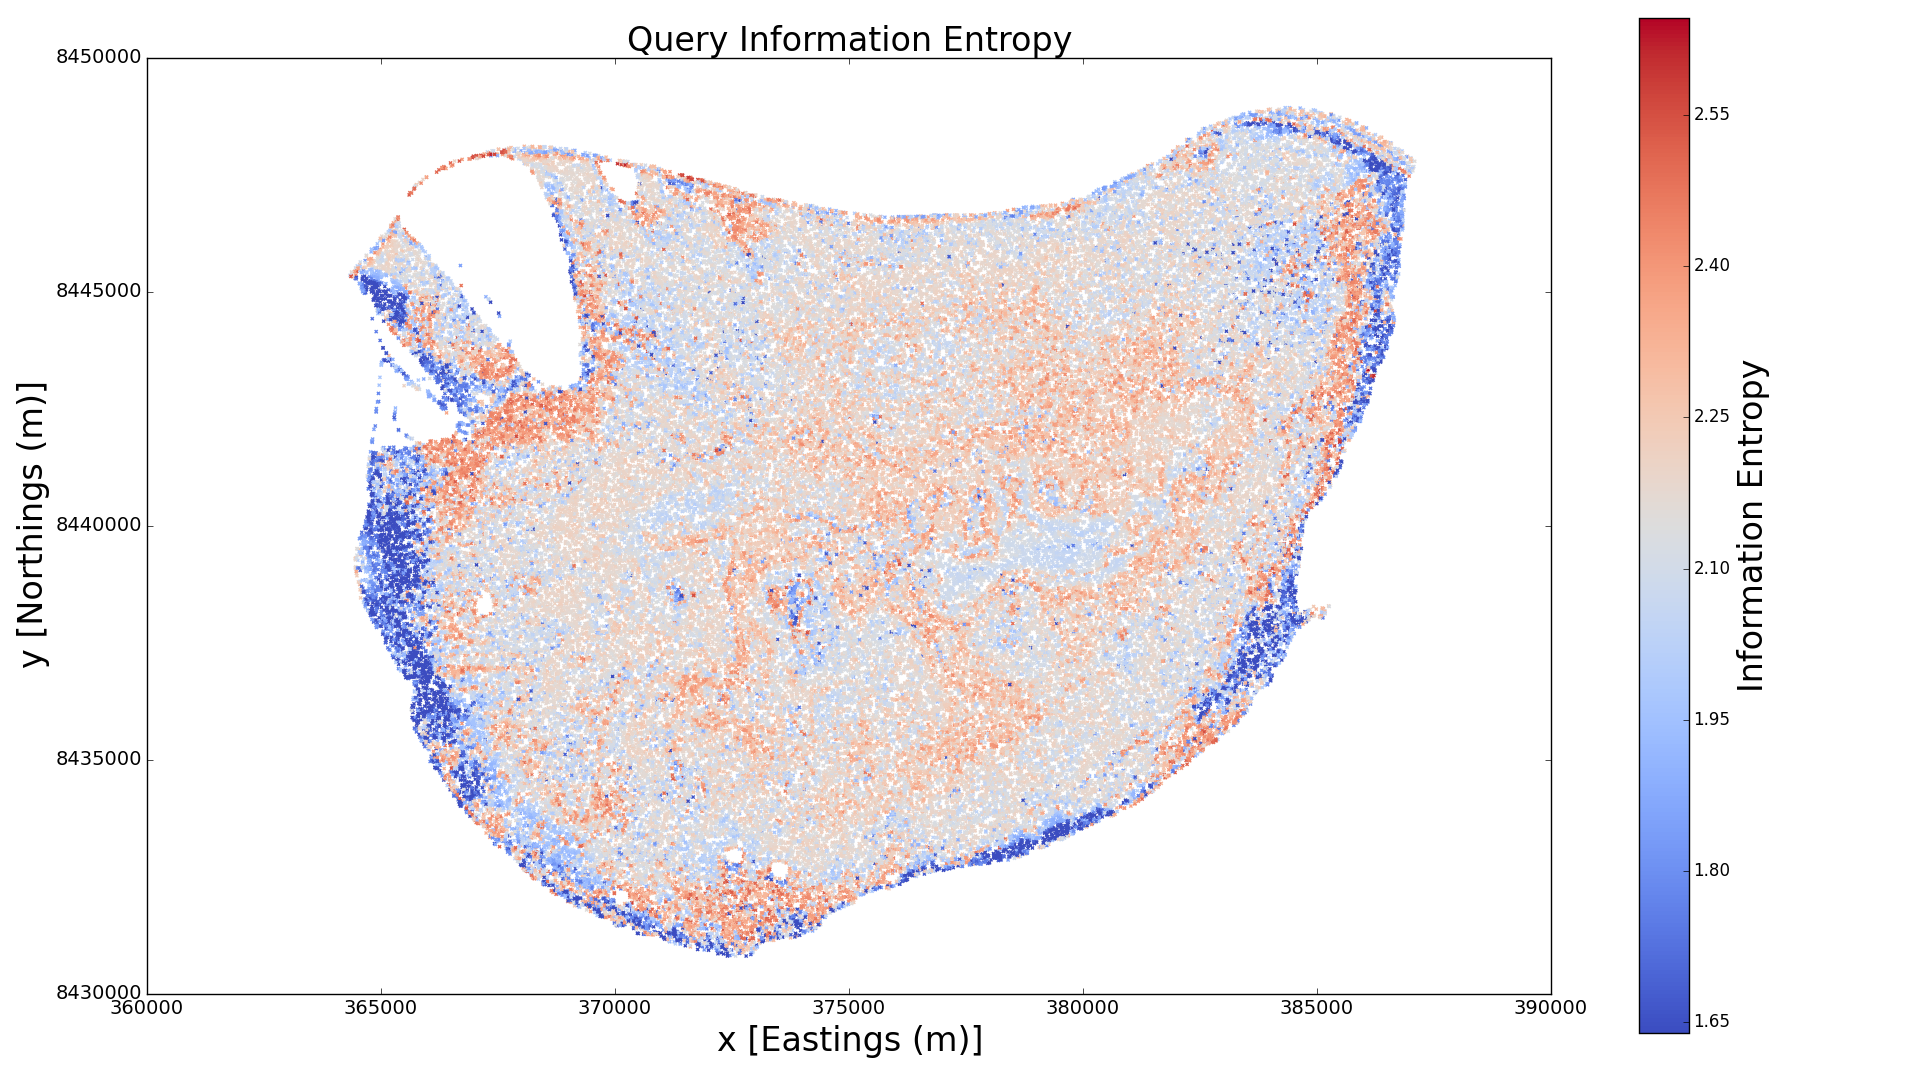
\includegraphics[width = \linewidth]{Figures/scott_reef_modeling/Figure9.png}
		\caption{Scott Reef: Prediction Information Entropy}
		\label{Figure:Results:ScottReefPredictionInformationEntropy}
		\end{figure}
					
		The linearised differential entropy, however, emphasizes on the places where the vehicle should first focus on (figure \ref{Figure:Results:ScottReefLinearisedDifferentialEntropy}). Comparing this with the bathymetric features (figure \ref{Figure:Results:ScottReefBathymetricFeatures}), we can deduce that the vehicle would focus on places with the highest and lowest depths. Notice that this is so even though the training data has covered the deepest parts of the reef.
		
		\begin{figure}[!htbp]
		\centering
			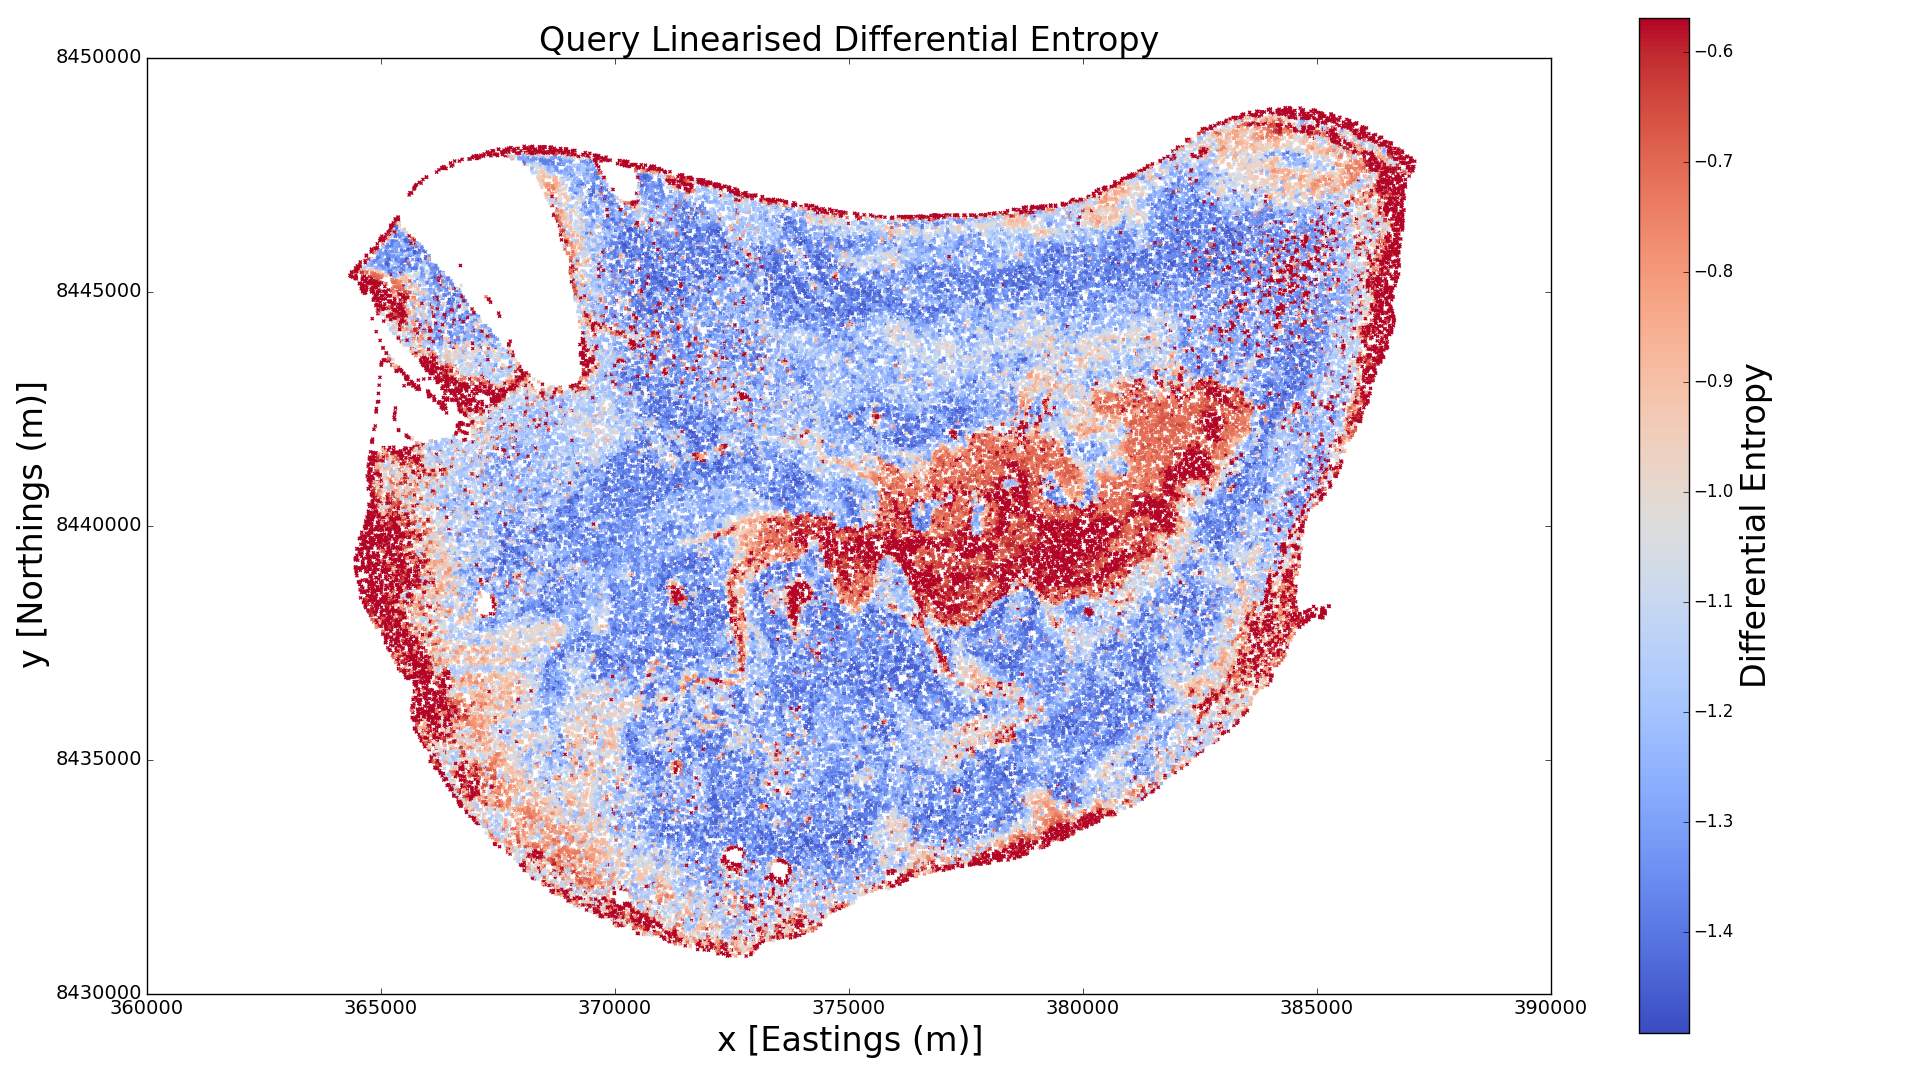
\includegraphics[width = \linewidth]{Figures/scott_reef_modeling/Figure11.png}
		\caption{Scott Reef: Linearised Differential Entropy}
		\label{Figure:Results:ScottReefLinearisedDifferentialEntropy}
		\end{figure}
	
		While these visualisations compare only the marginalised entropies at each query point, the main advantage of using linearised differential entropy as the acquisition function is that the joint linearised differential entropy between an arbitrary set of query points can be readily computed in a straight forward way by \eqref{Section:LinearisedEntropy:Equation:BinaryLinearisedEntropy} and \eqref{Section:LinearisedEntropy:Equation:MulticlassLinearisedEntropy}. On the other hand, there are no closed form for the joint prediction information entropy, so one would have to use Monte Carlo sampling to estimate the joint distributions. Thus, the accuracy of the mutual entropy measure would depend on the number of sample draws used for the estimation. On top of the properties of the marginalised prediction information entropy discussed earlier, this can make the method of Monte Carlo sampling less desirable.
			
	\subsection{Exploration over Scott Reef Benthic Habitats}
	
		\begin{figure*}[!htbp]
		\centering
			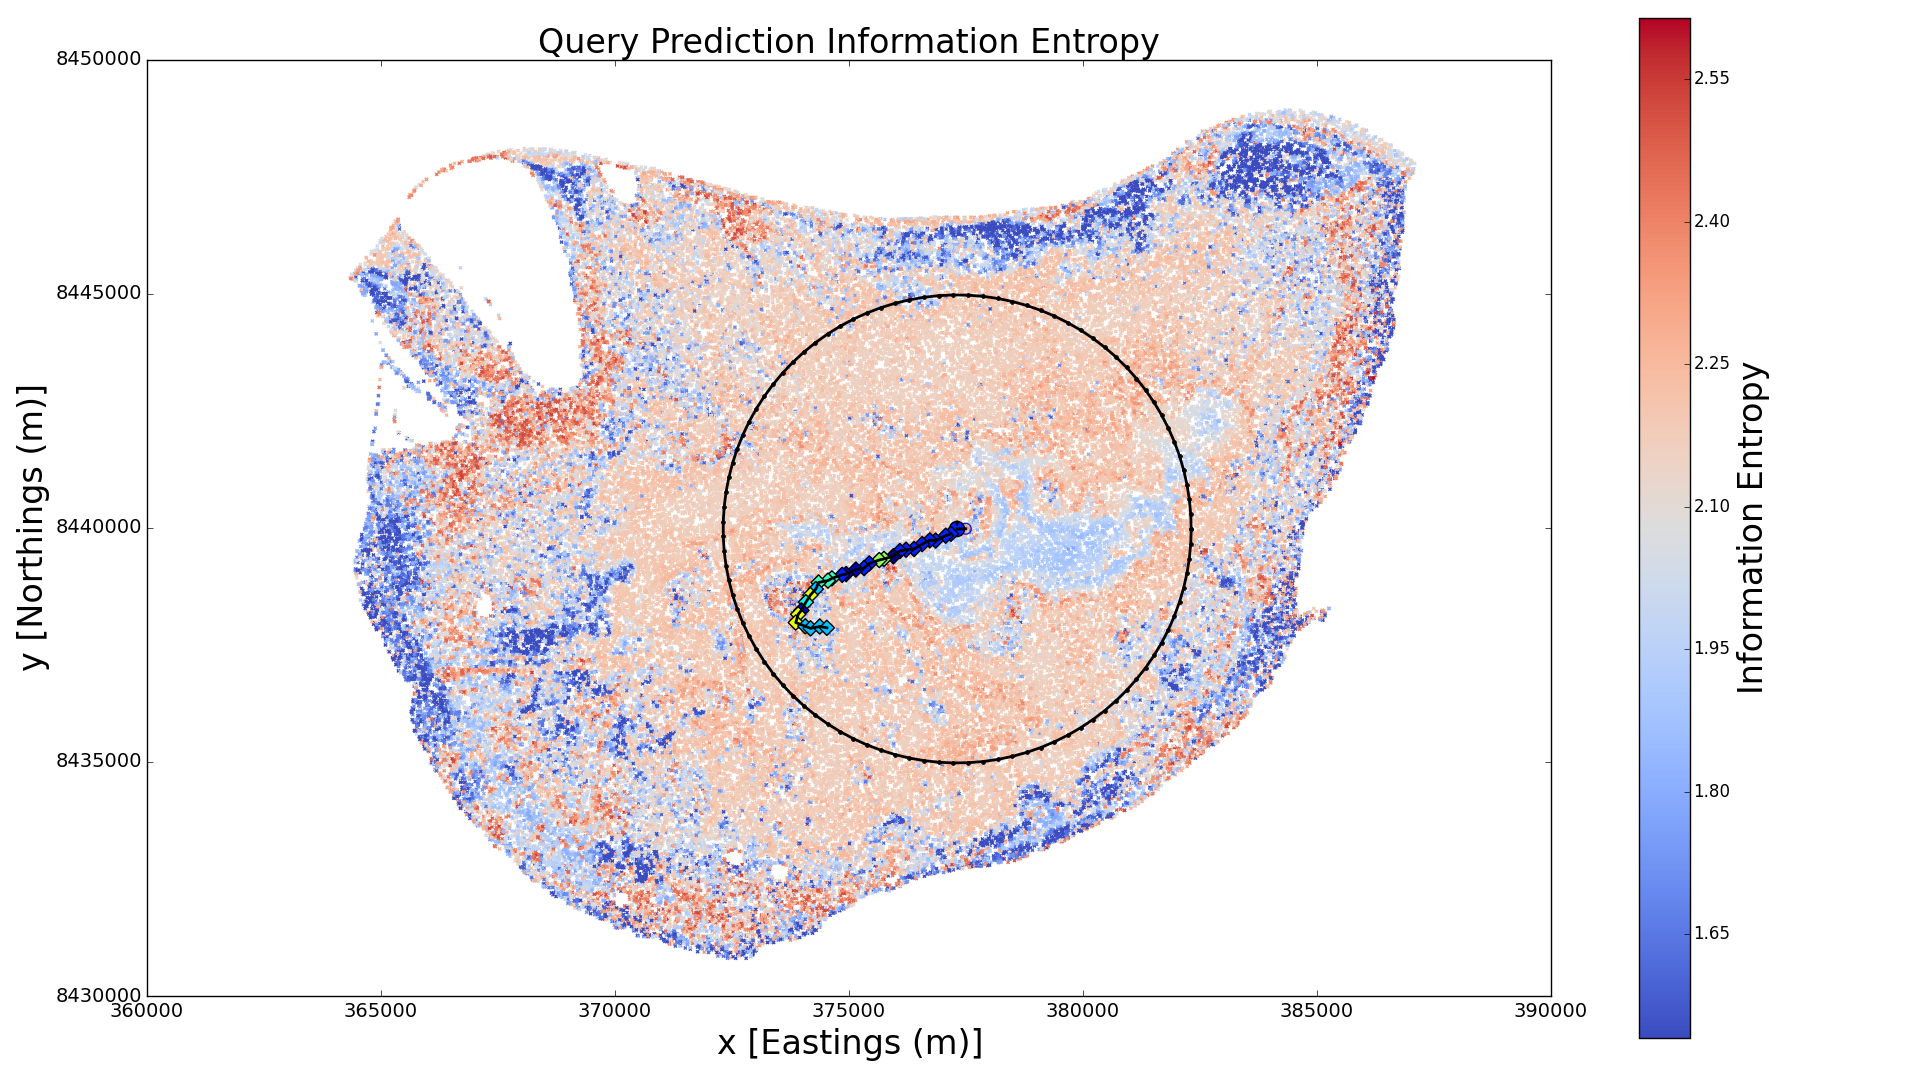
\includegraphics[width = 0.24\linewidth]{Figures/location_1_lde_path/mie_propose_step1.png}
			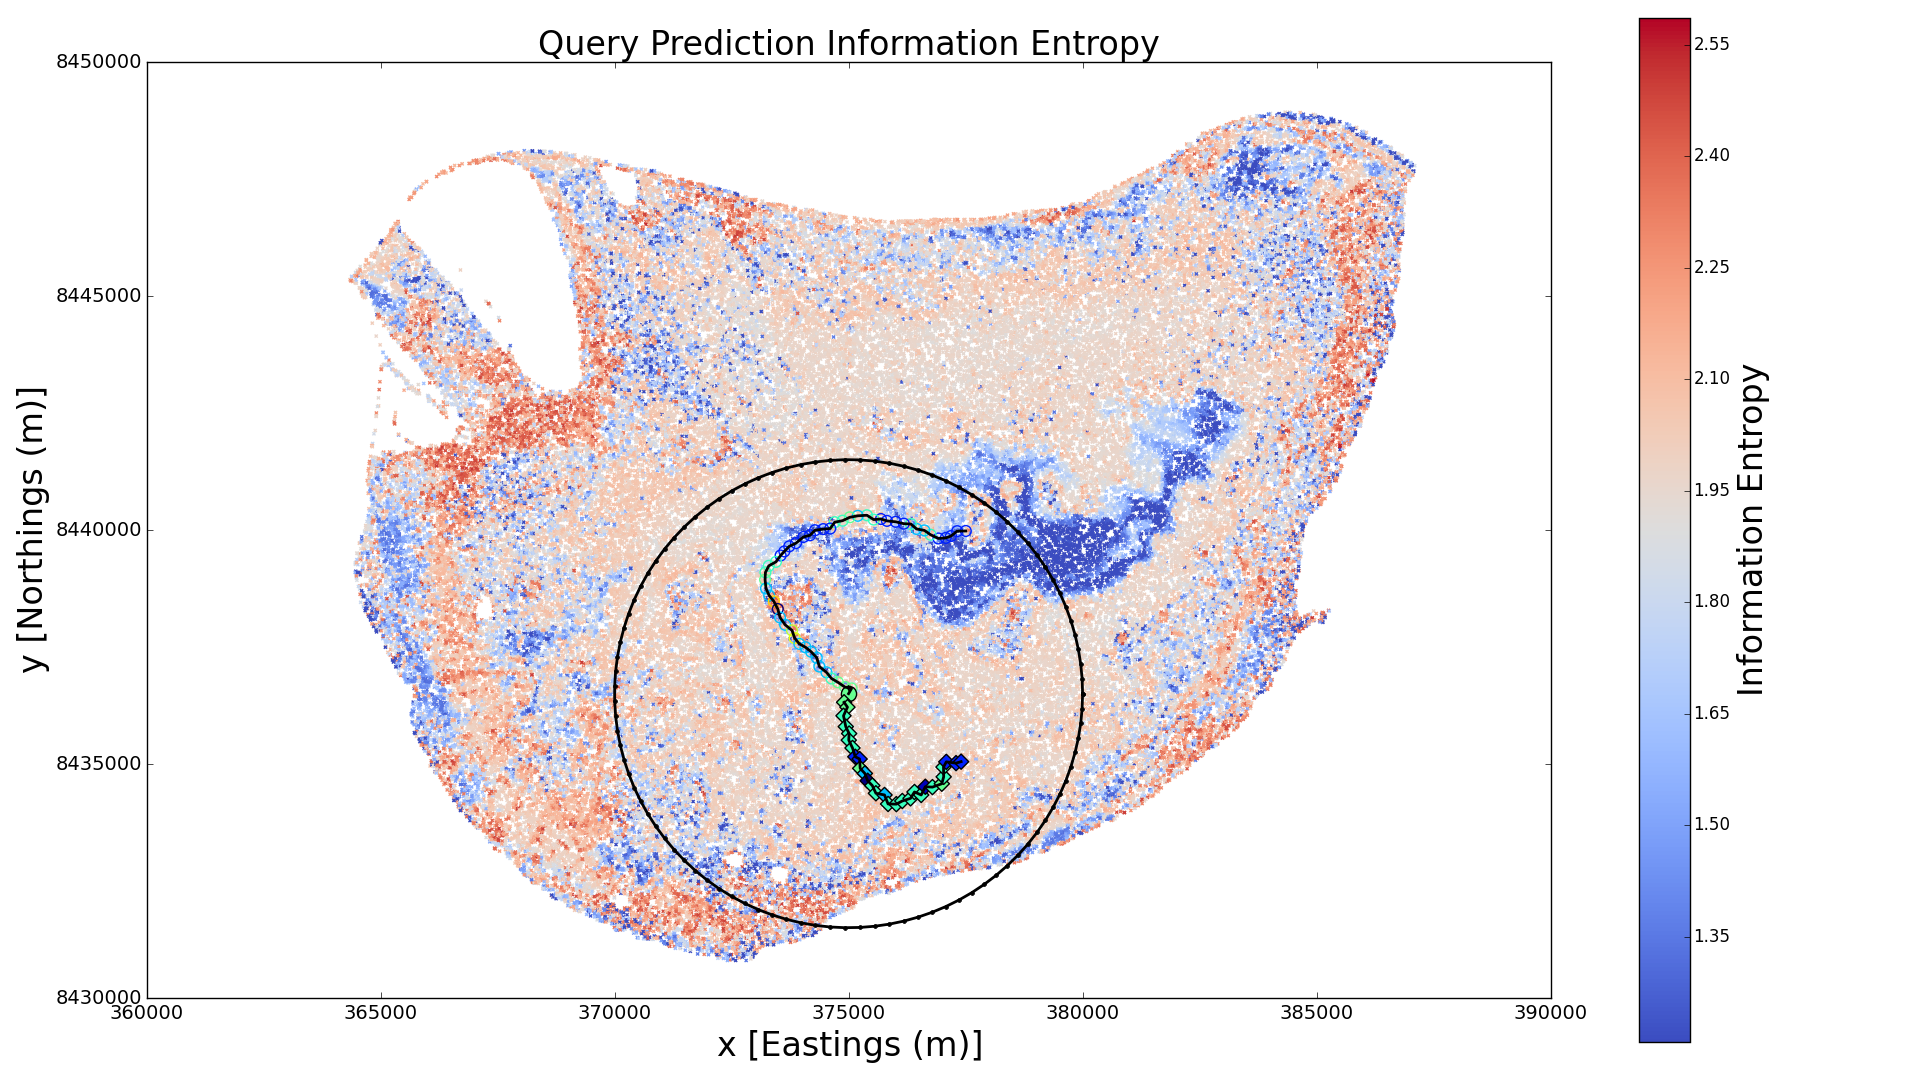
\includegraphics[width = 0.24\linewidth]{Figures/location_1_lde_path/mie_propose_step50.png}
			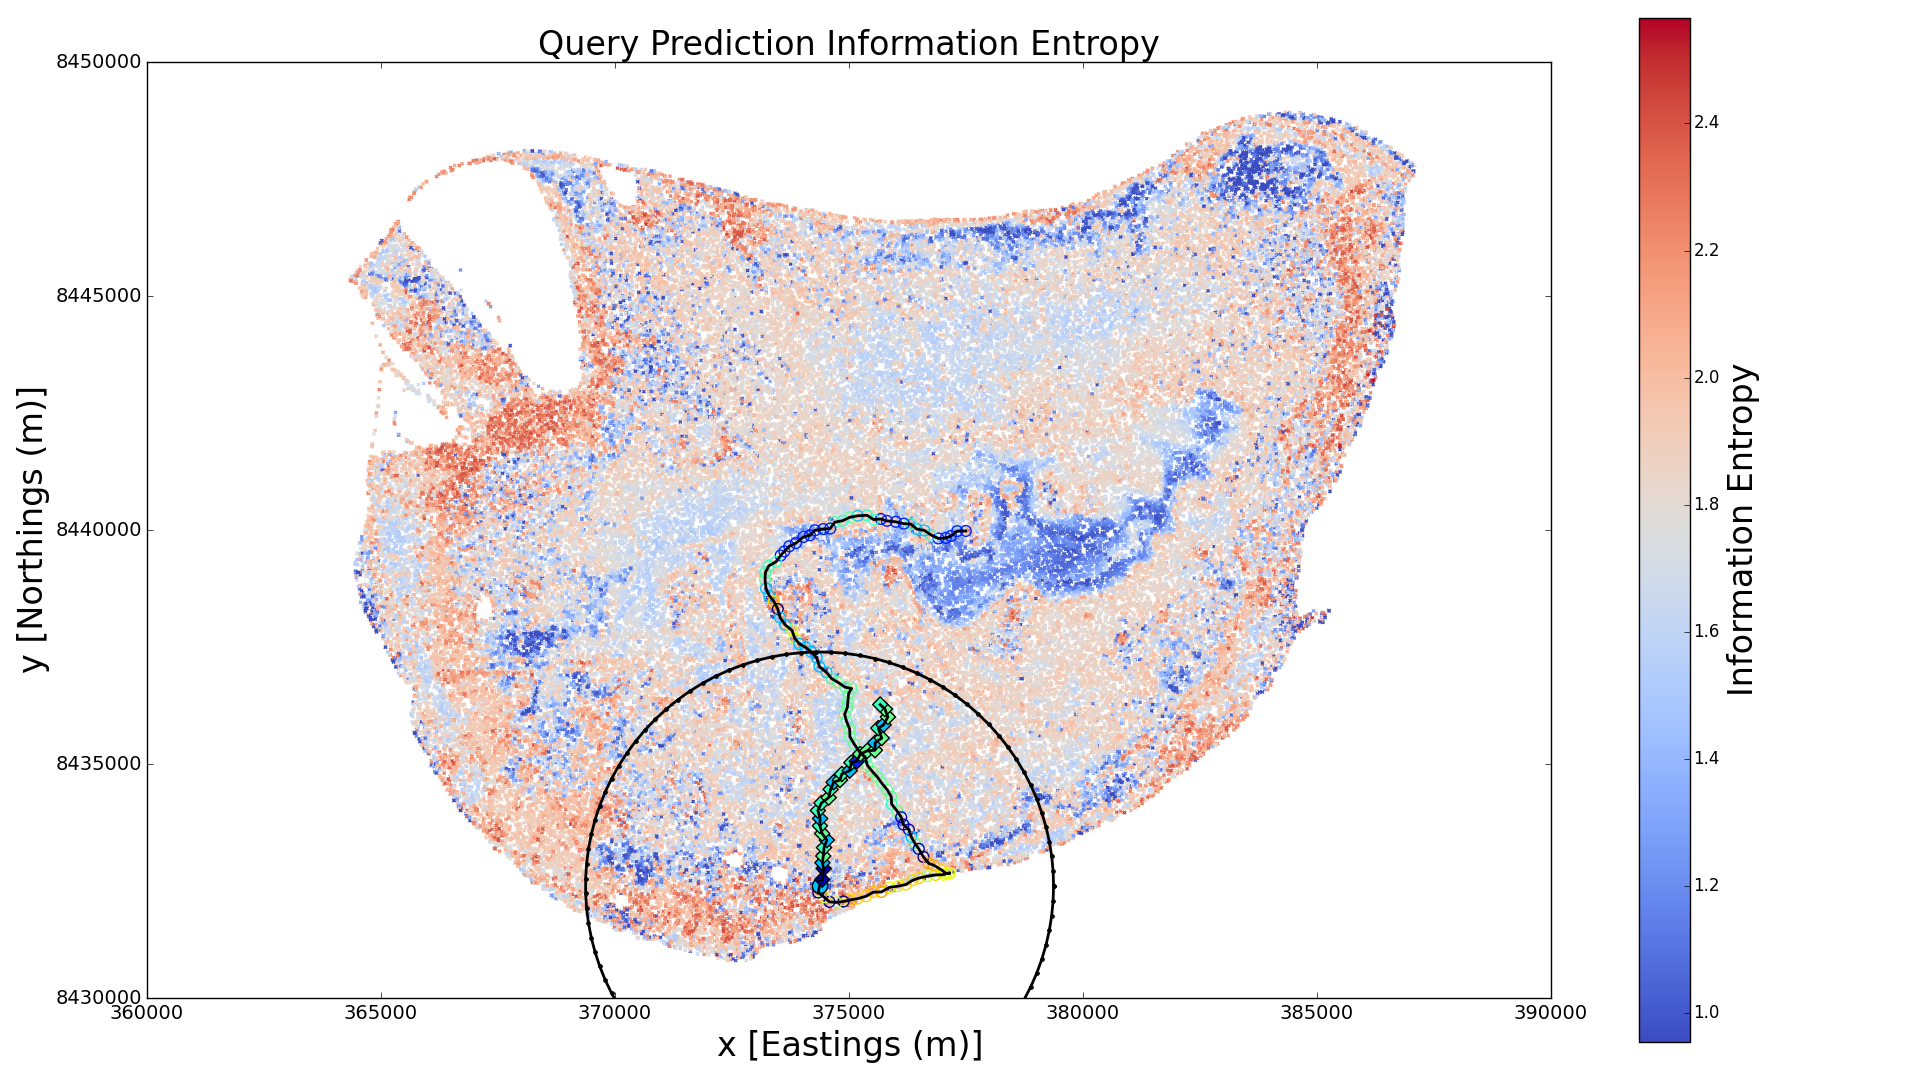
\includegraphics[width = 0.24\linewidth]{Figures/location_1_lde_path/mie_propose_step100.png}
			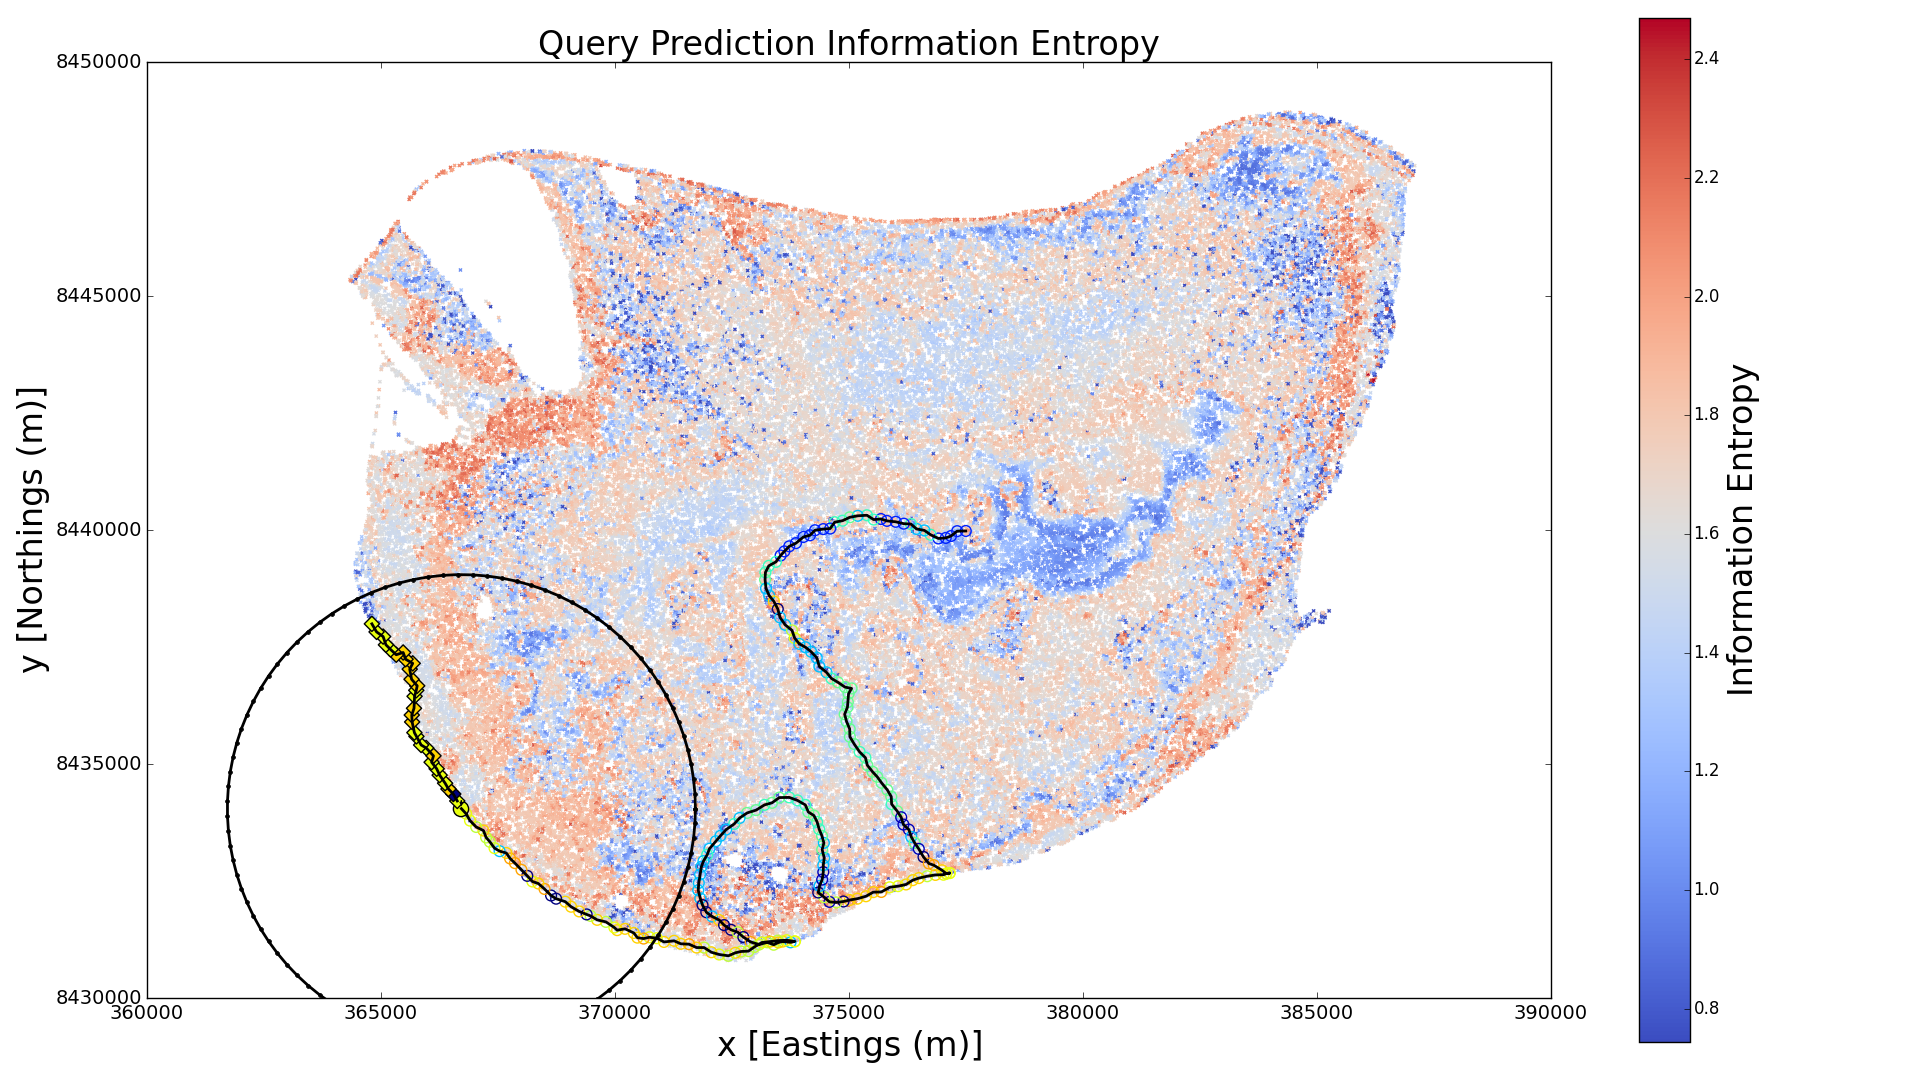
\includegraphics[width = 0.24\linewidth]{Figures/location_1_lde_path/mie_propose_step200.png}
			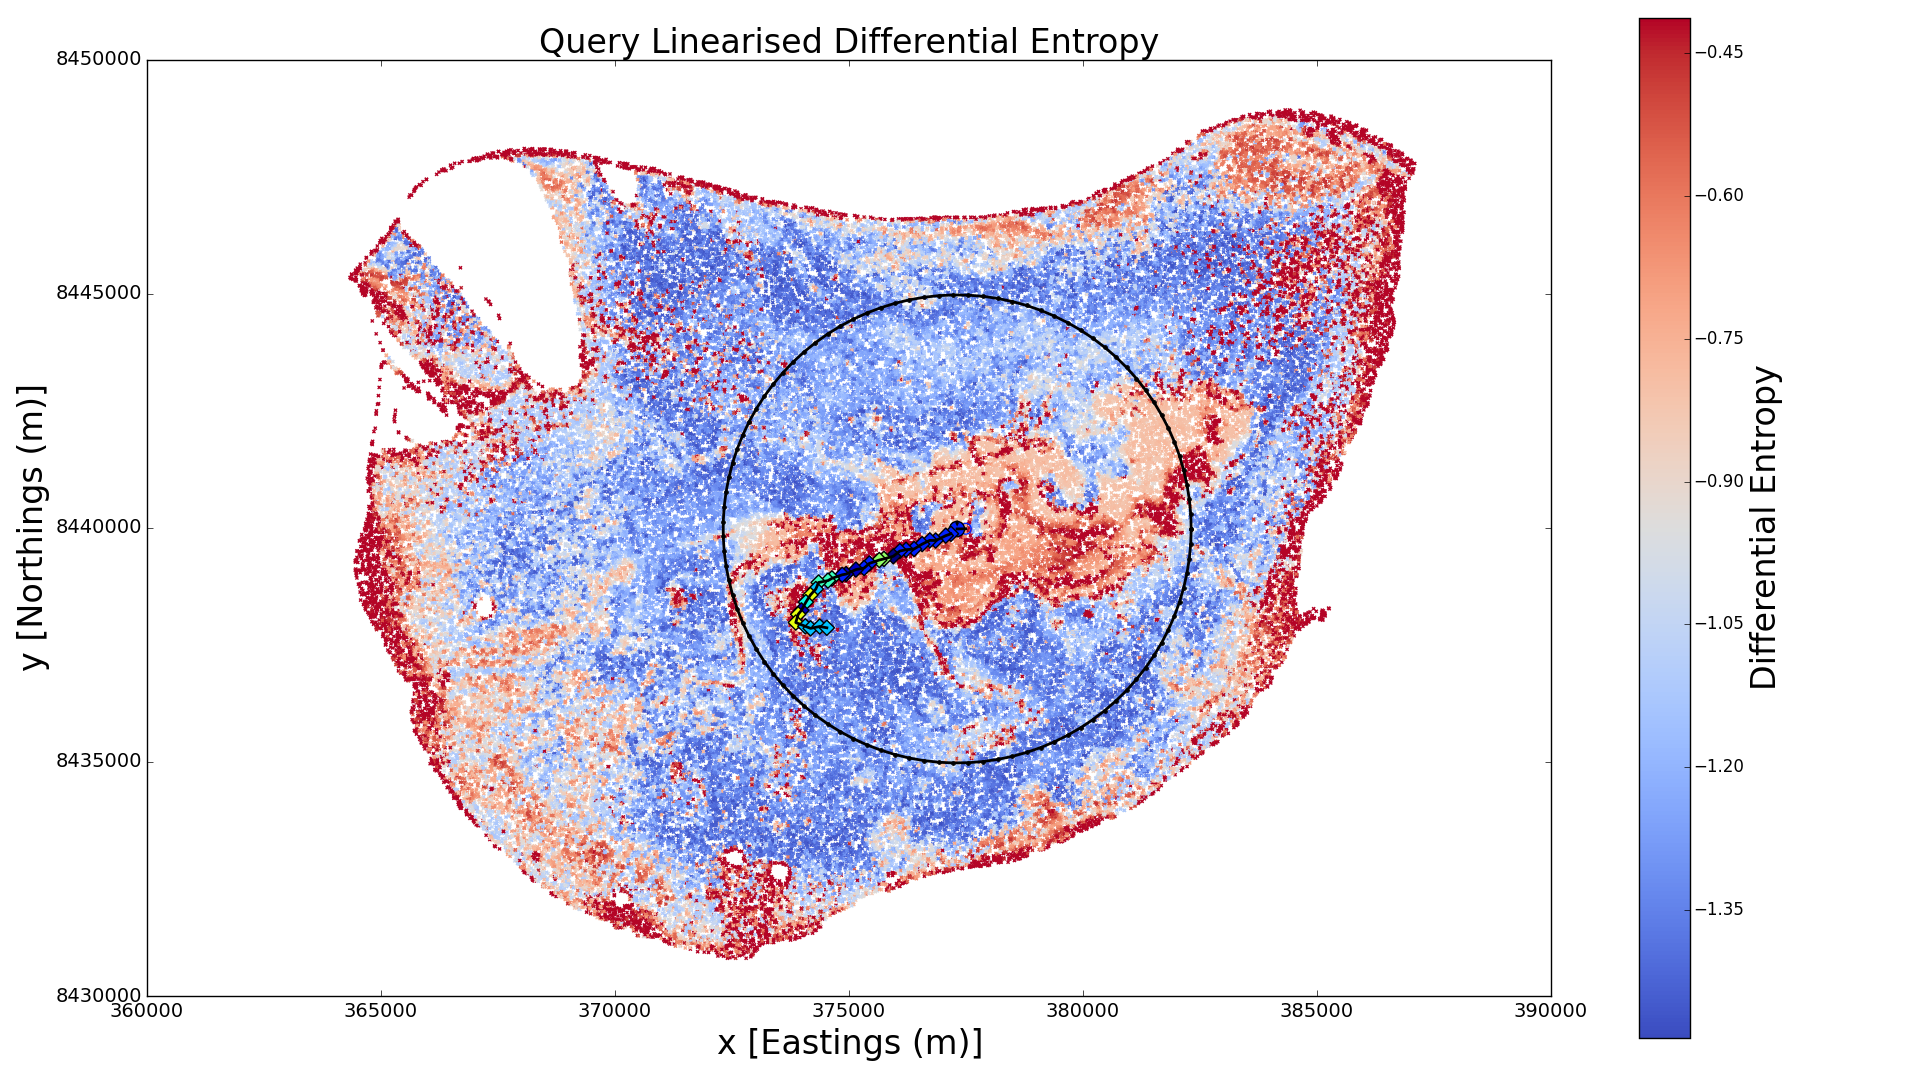
\includegraphics[width = 0.24\linewidth]{Figures/location_1_lde_path/lde_propose_step1.png}
			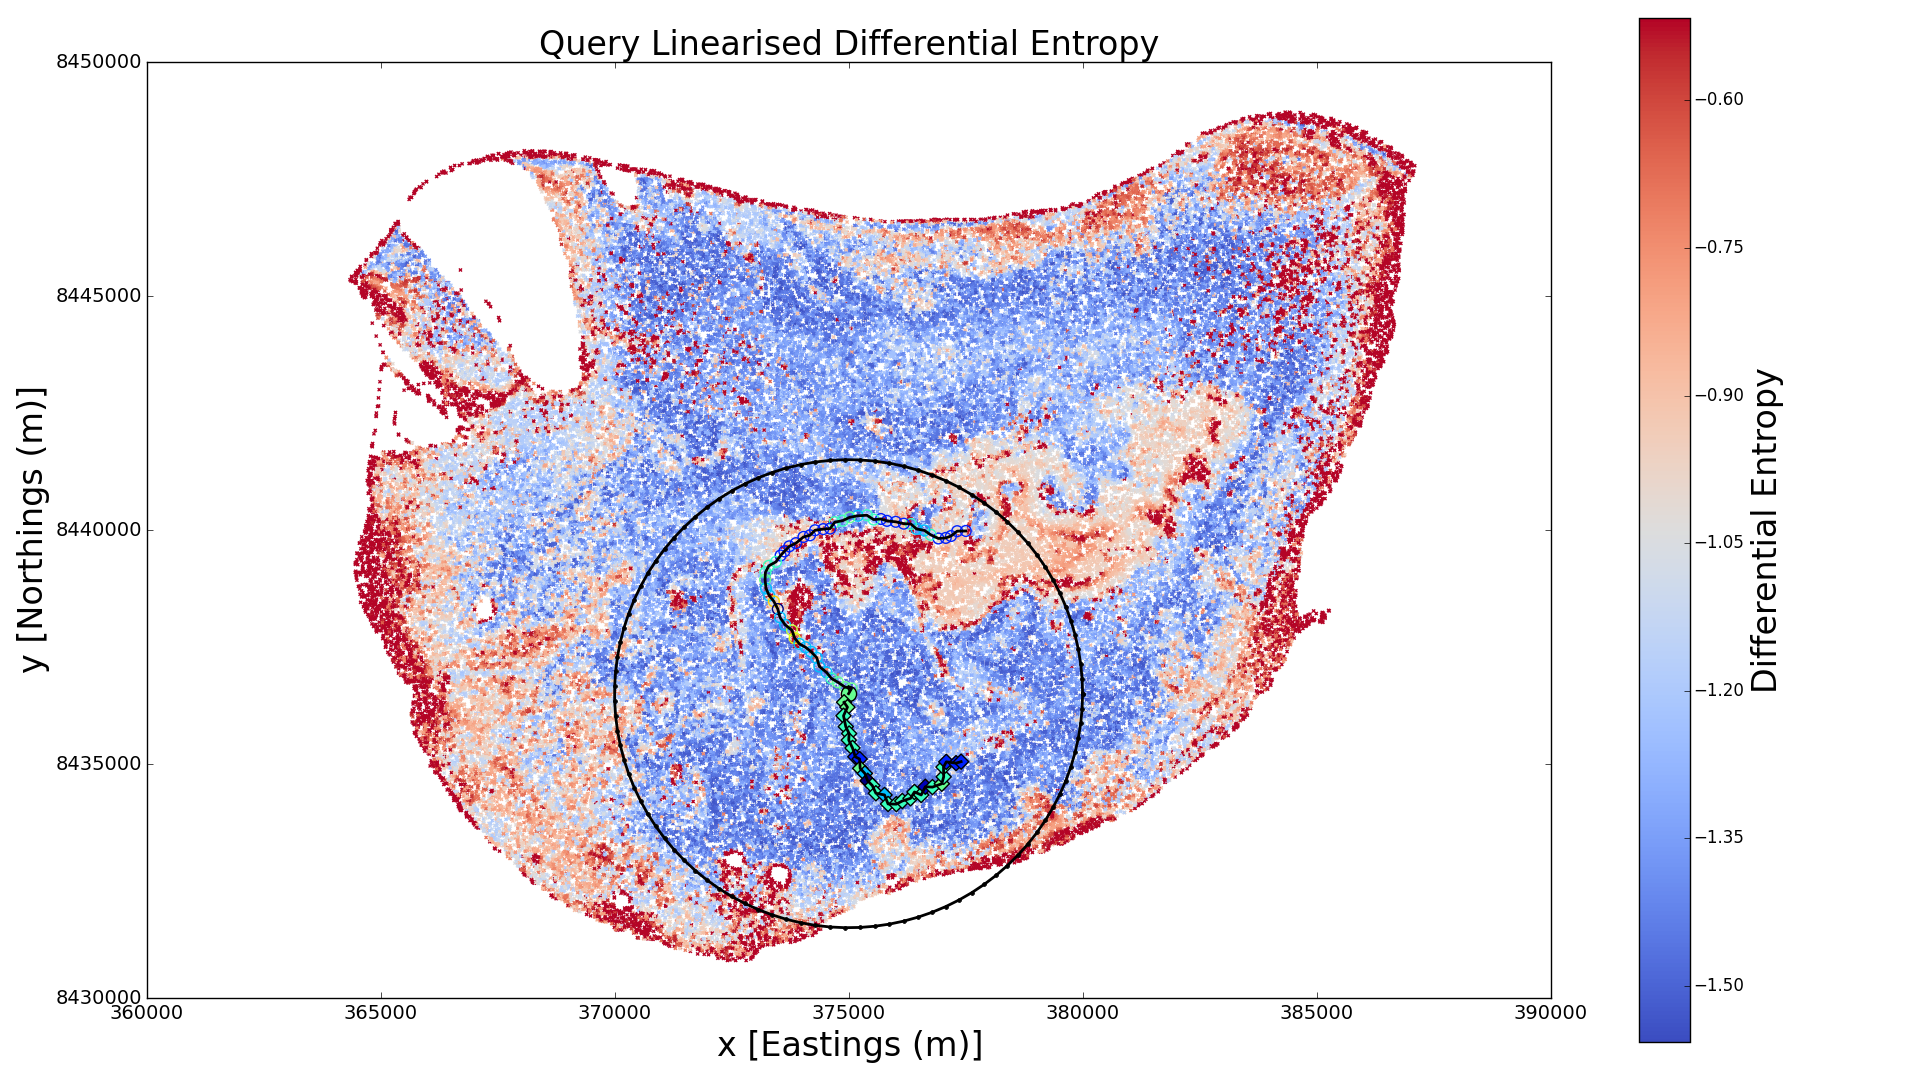
\includegraphics[width = 0.24\linewidth]{Figures/location_1_lde_path/lde_propose_step50.png}
			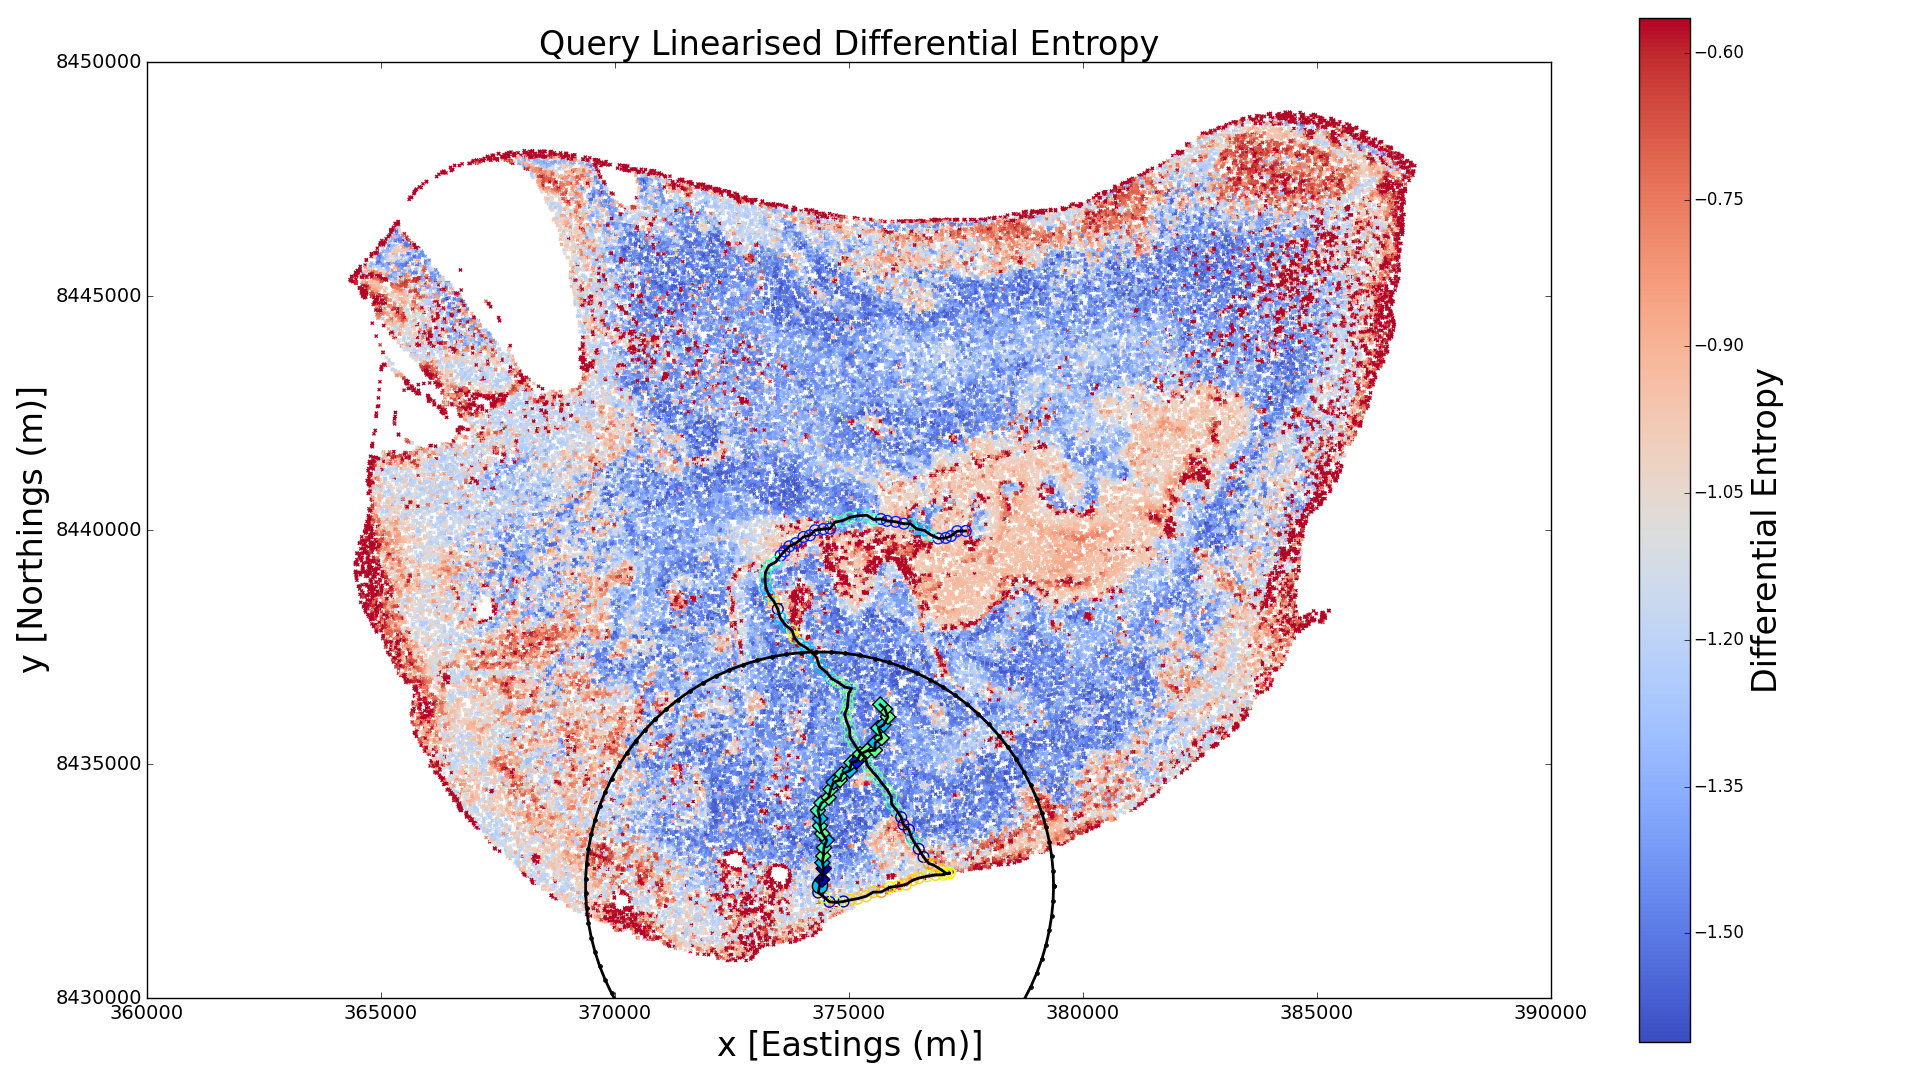
\includegraphics[width = 0.24\linewidth]{Figures/location_1_lde_path/lde_propose_step100.png}
			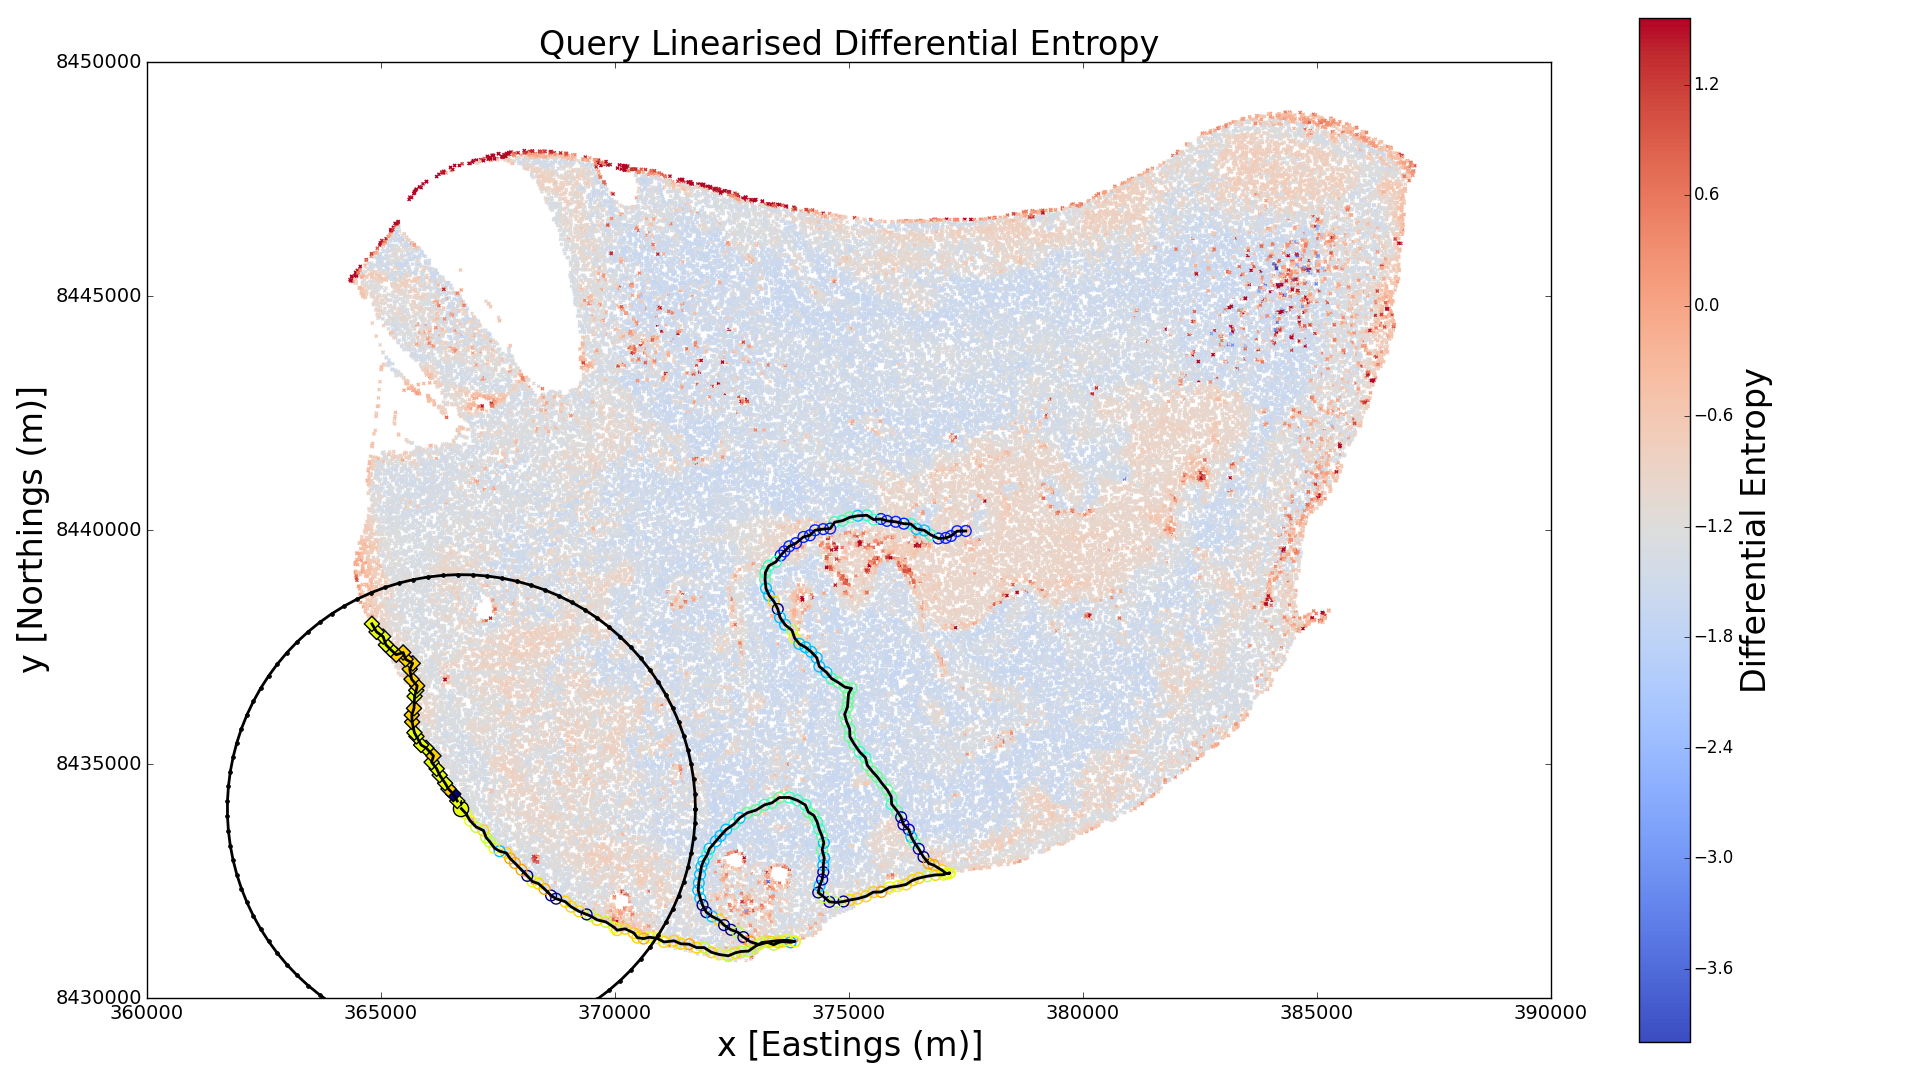
\includegraphics[width = 0.24\linewidth]{Figures/location_1_lde_path/lde_propose_step200.png}
			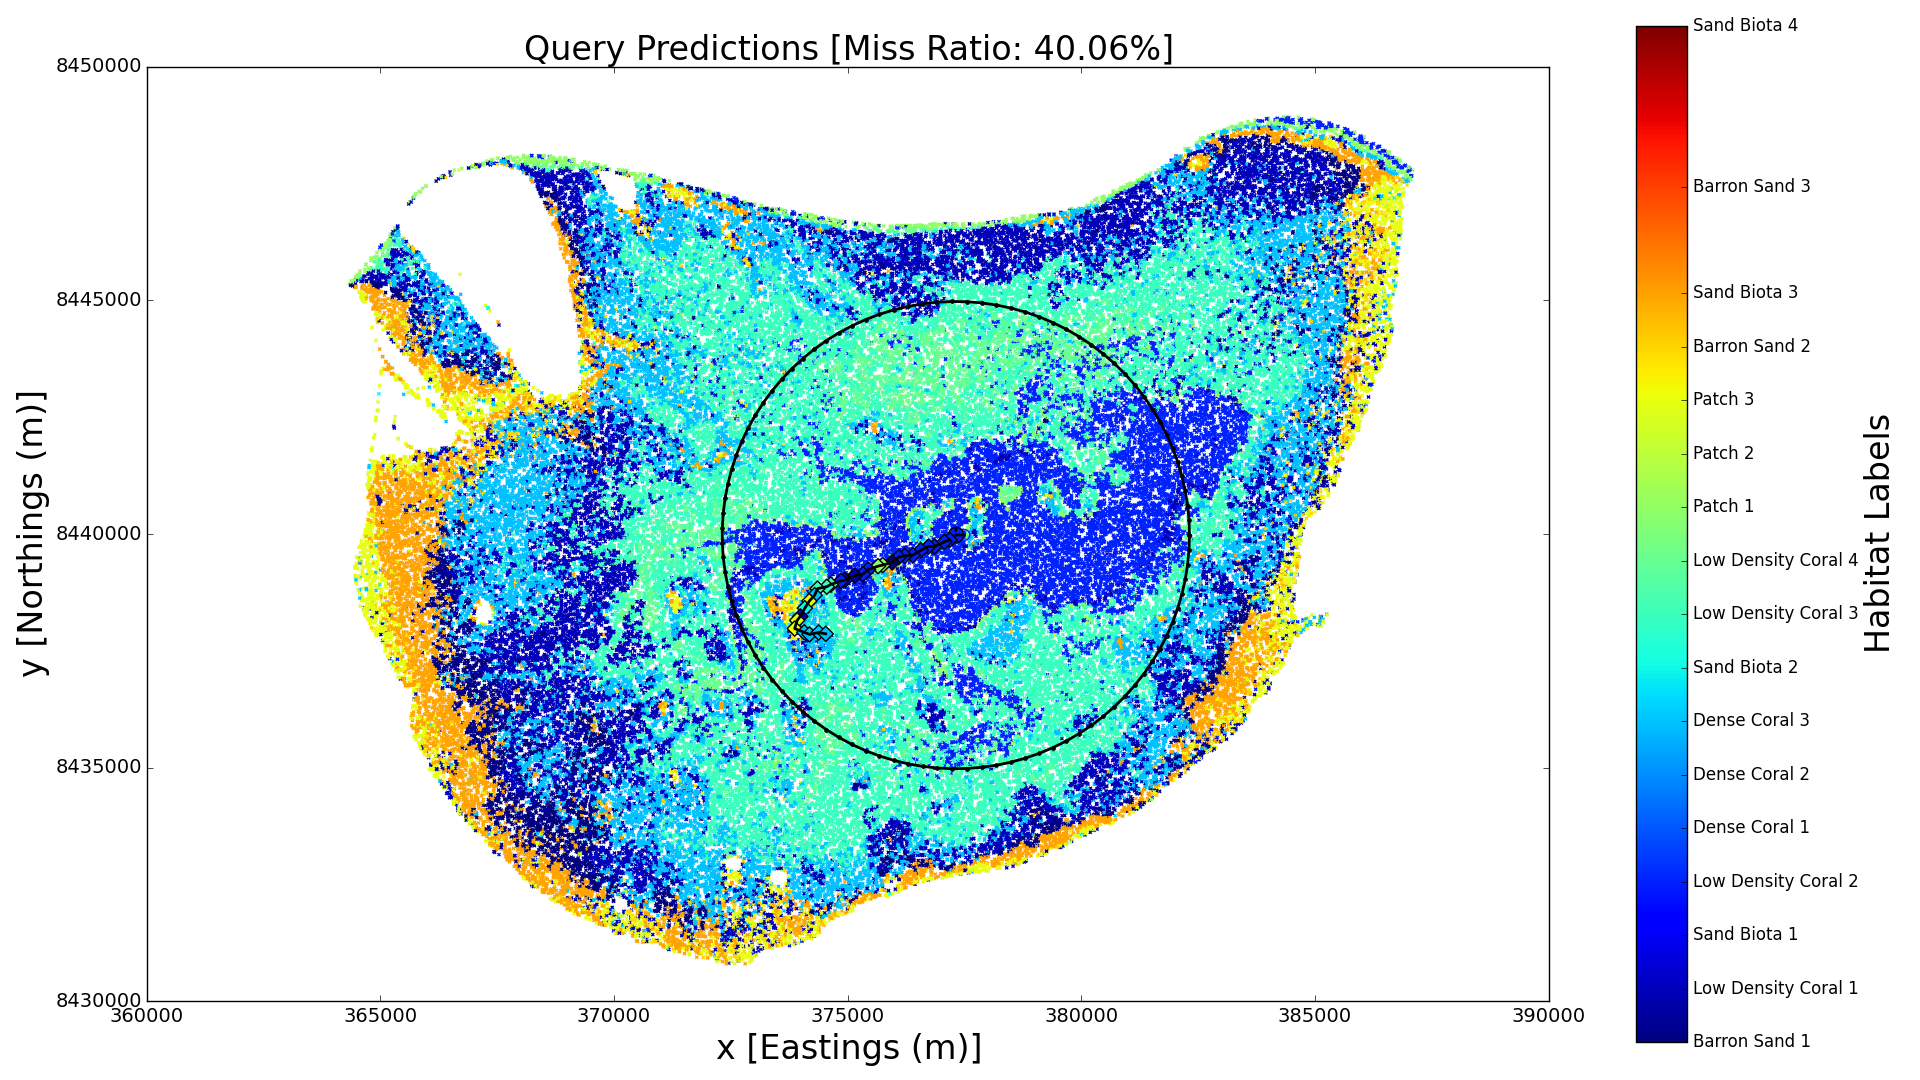
\includegraphics[width = 0.24\linewidth]{Figures/location_1_lde_path/pred_propose_step1.png}
			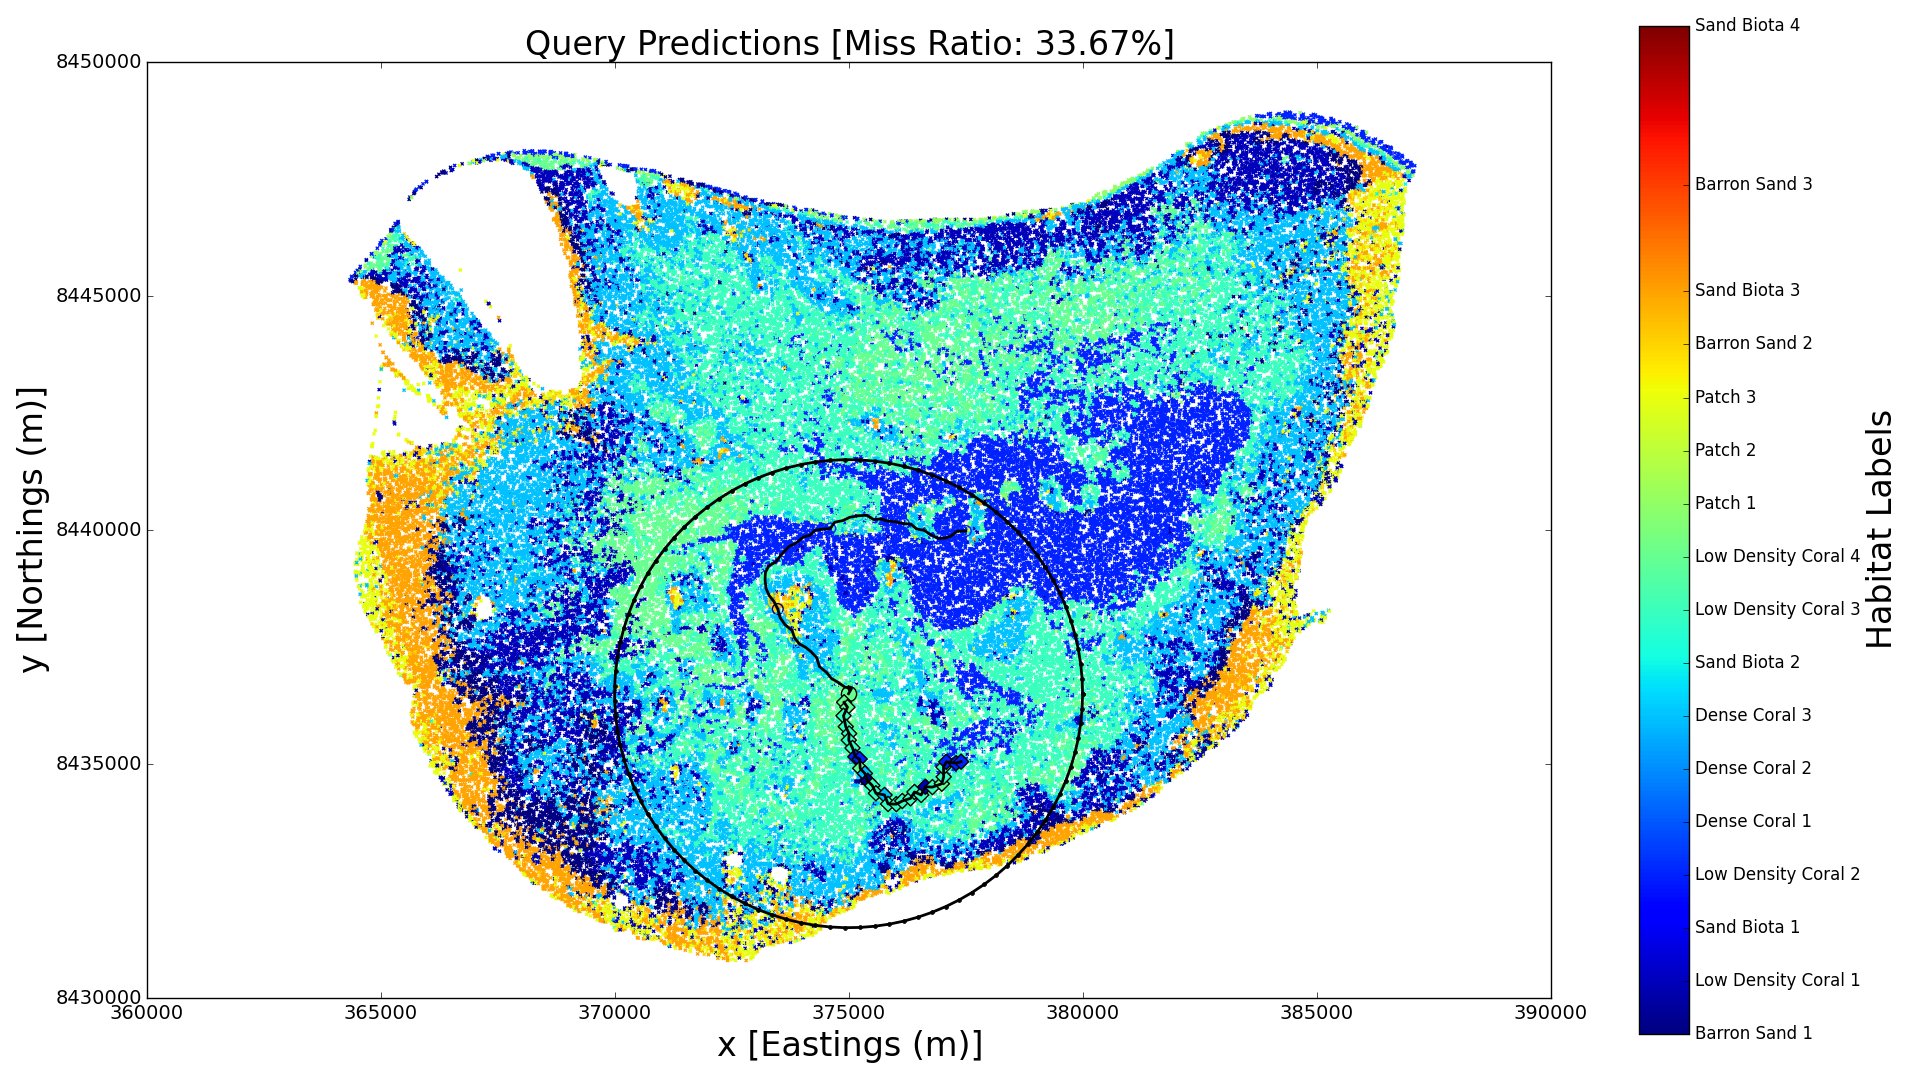
\includegraphics[width = 0.24\linewidth]{Figures/location_1_lde_path/pred_propose_step50.png}
			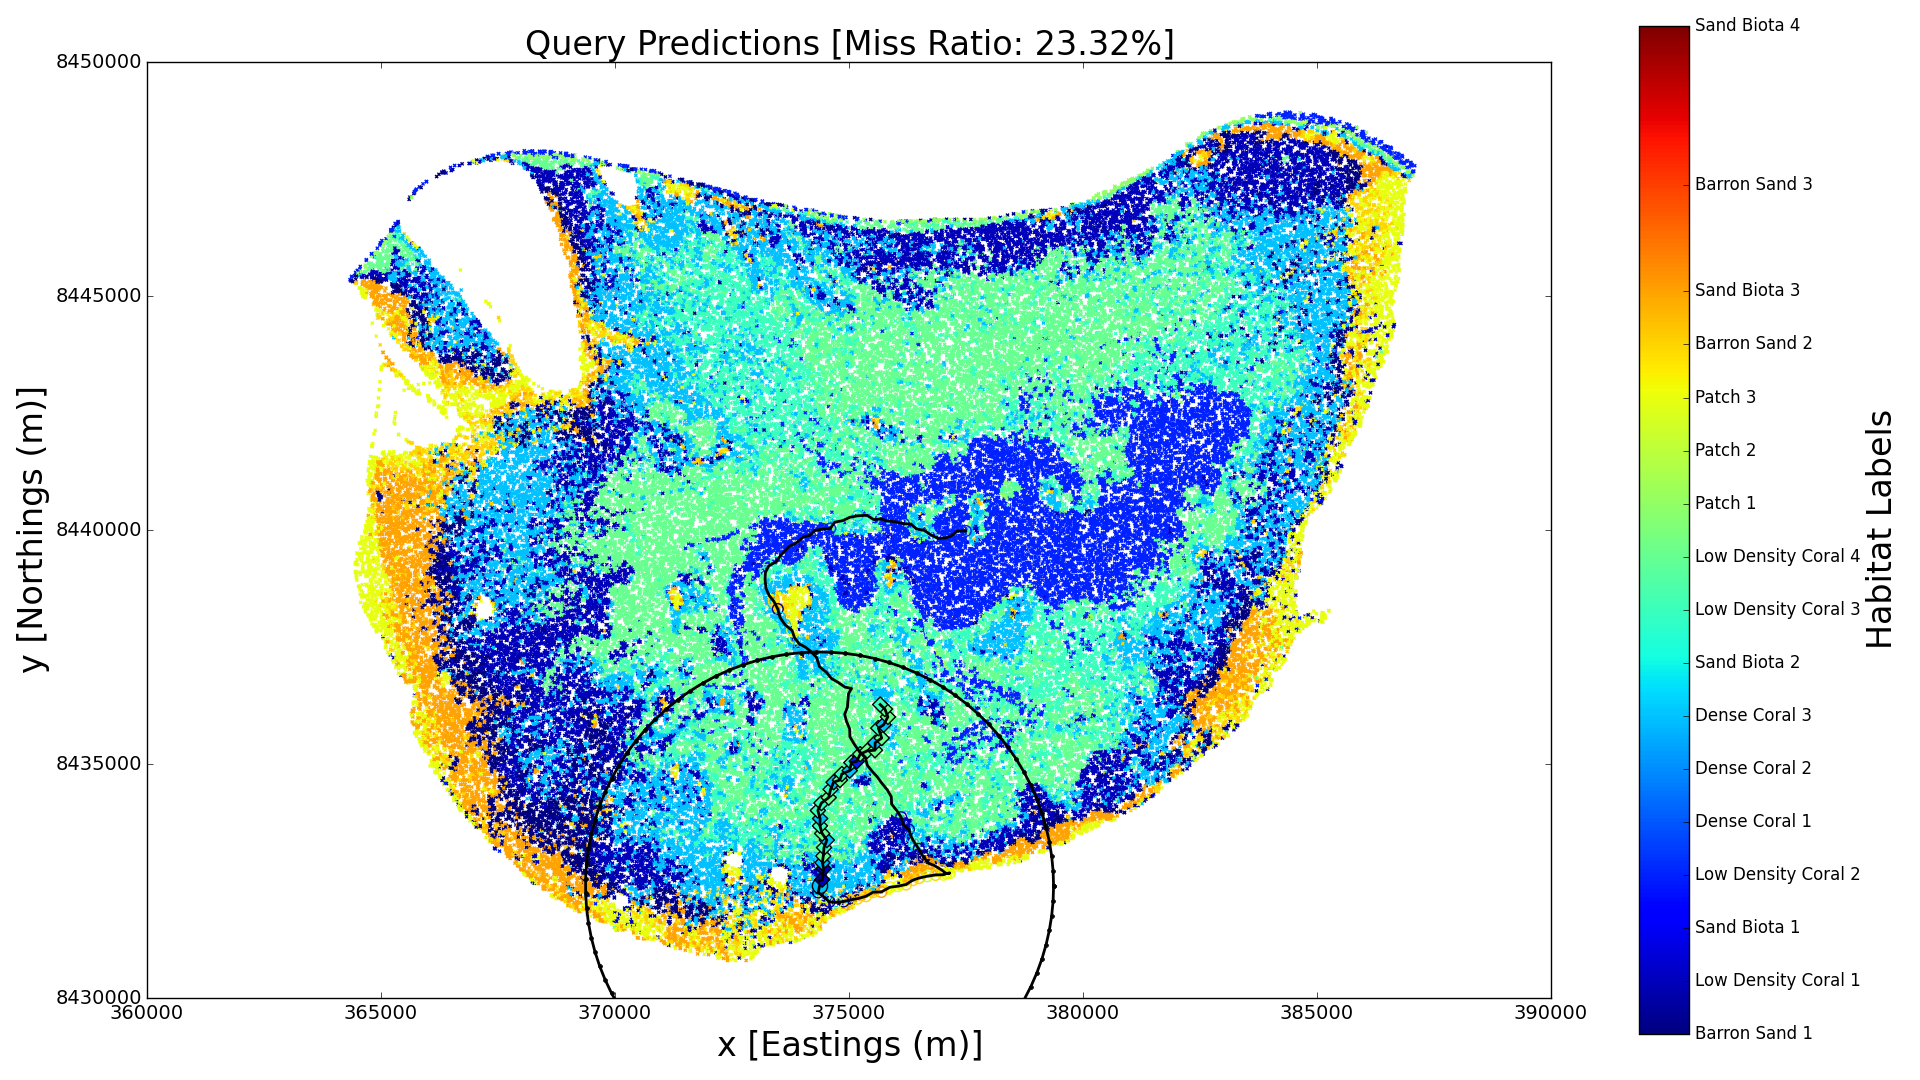
\includegraphics[width = 0.24\linewidth]{Figures/location_1_lde_path/pred_propose_step100.png}
			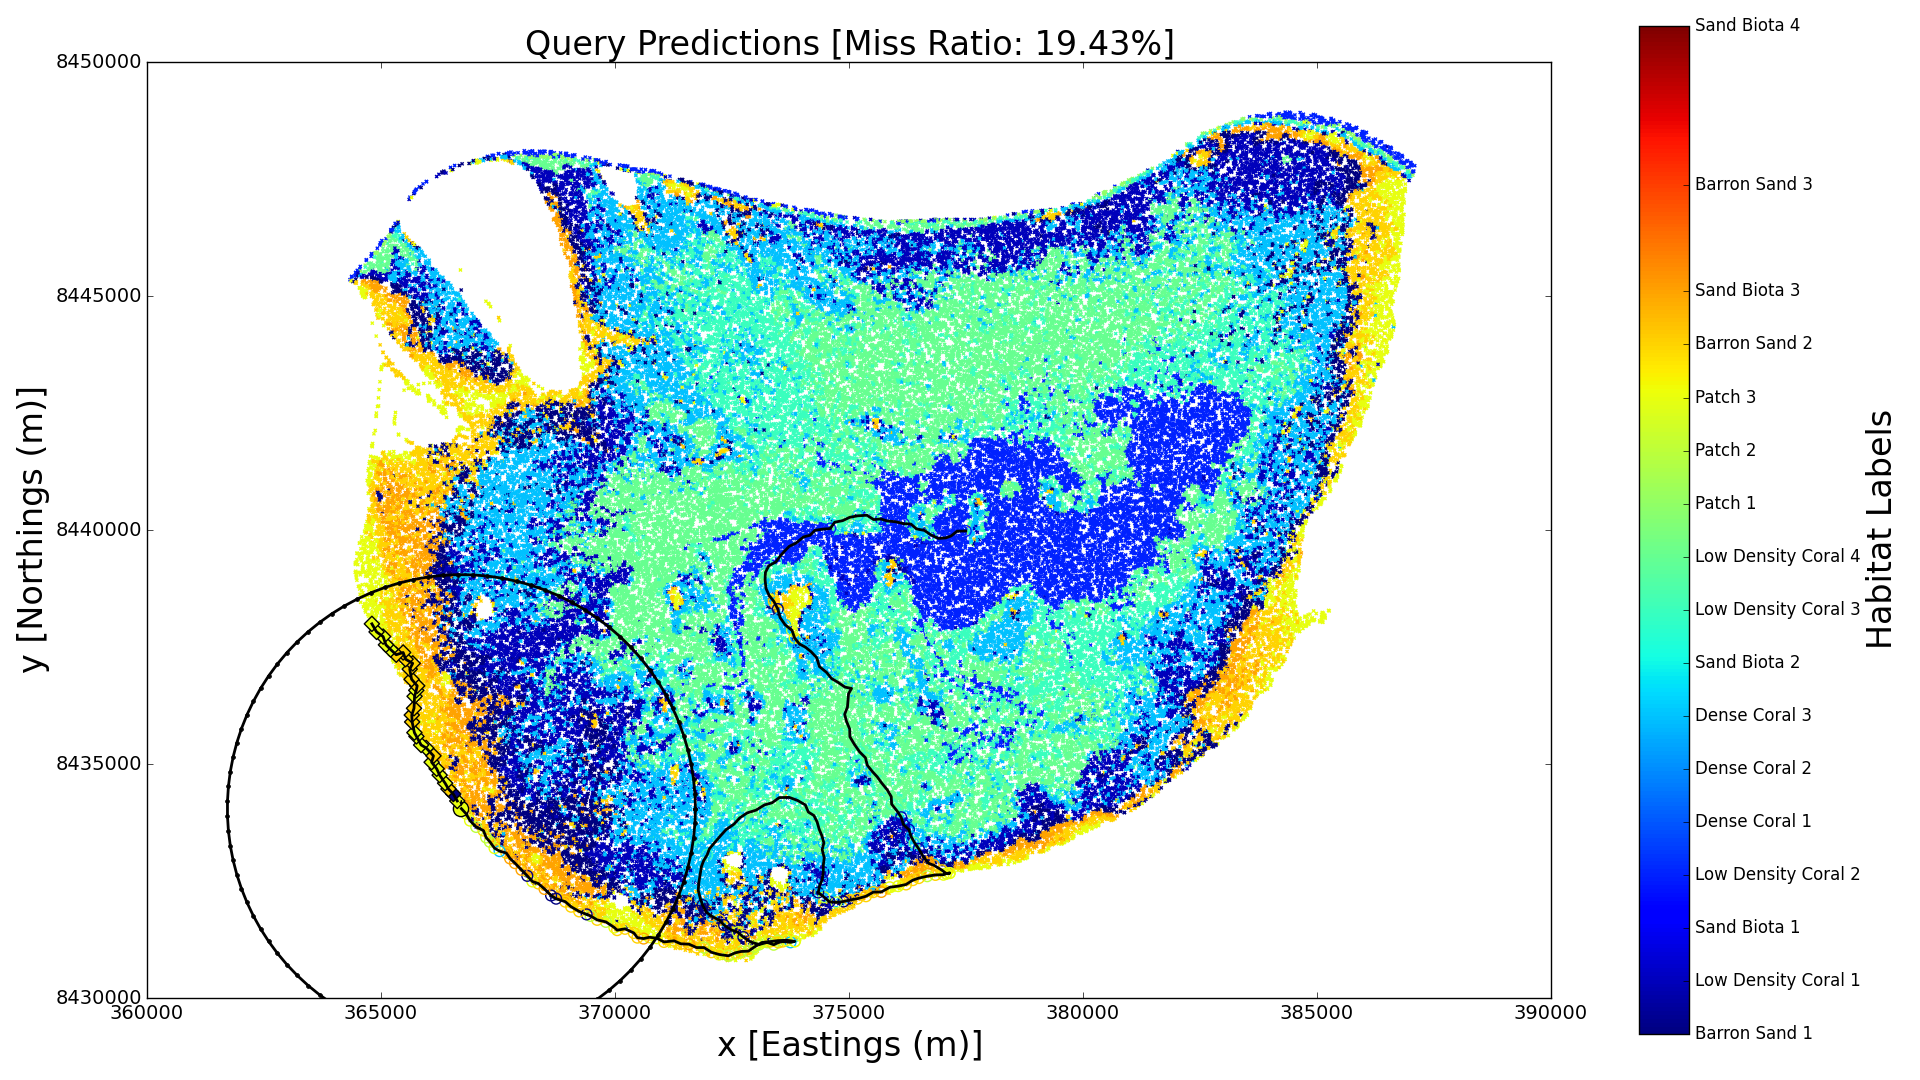
\includegraphics[width = 0.24\linewidth]{Figures/location_1_lde_path/pred_propose_step200.png}			
		\caption{Exploration path under linearised differential entropy acquisition}
		\label{Figure:Results:OptimalPathLDE}
		\end{figure*}

		\begin{figure*}[!htbp]
		\centering
			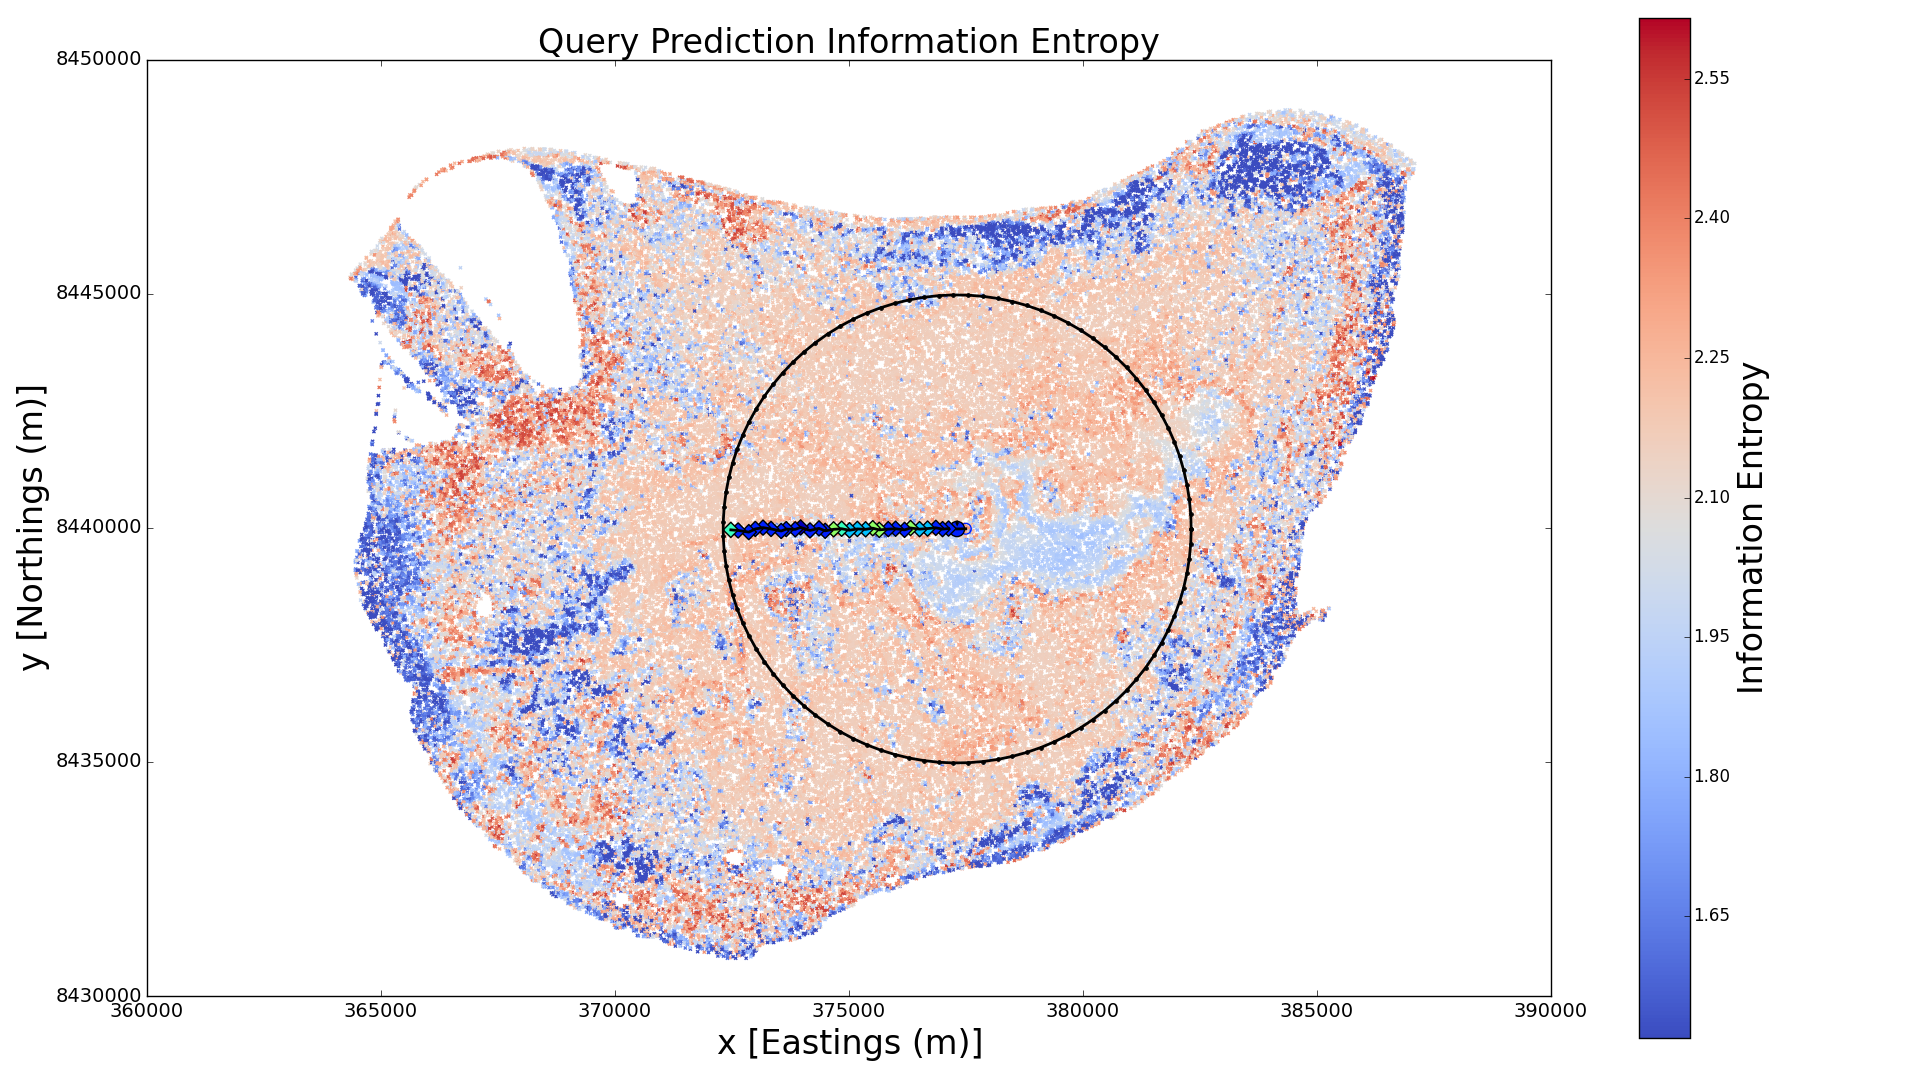
\includegraphics[width = 0.24\linewidth]{Figures/location_1_mcje_path/mie_propose_step1.png}
			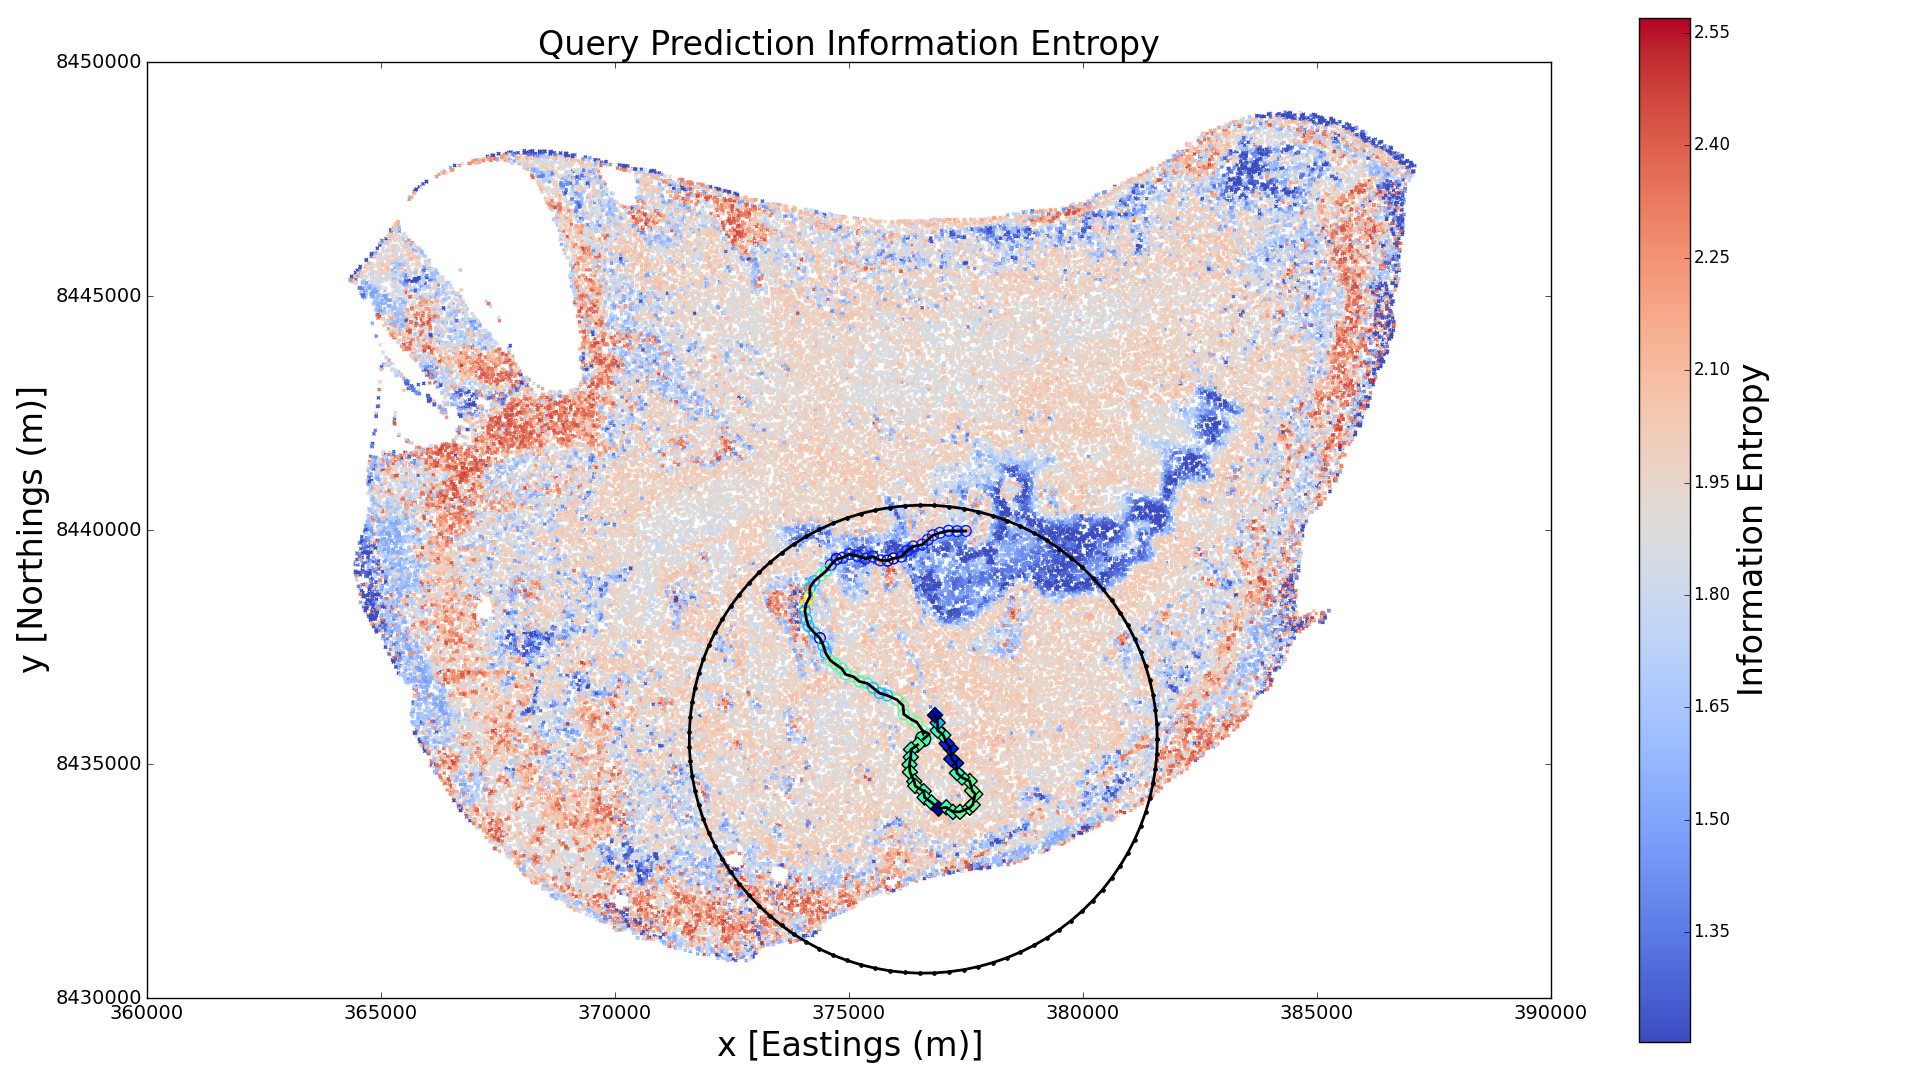
\includegraphics[width = 0.24\linewidth]{Figures/location_1_mcje_path/mie_propose_step50.png}
			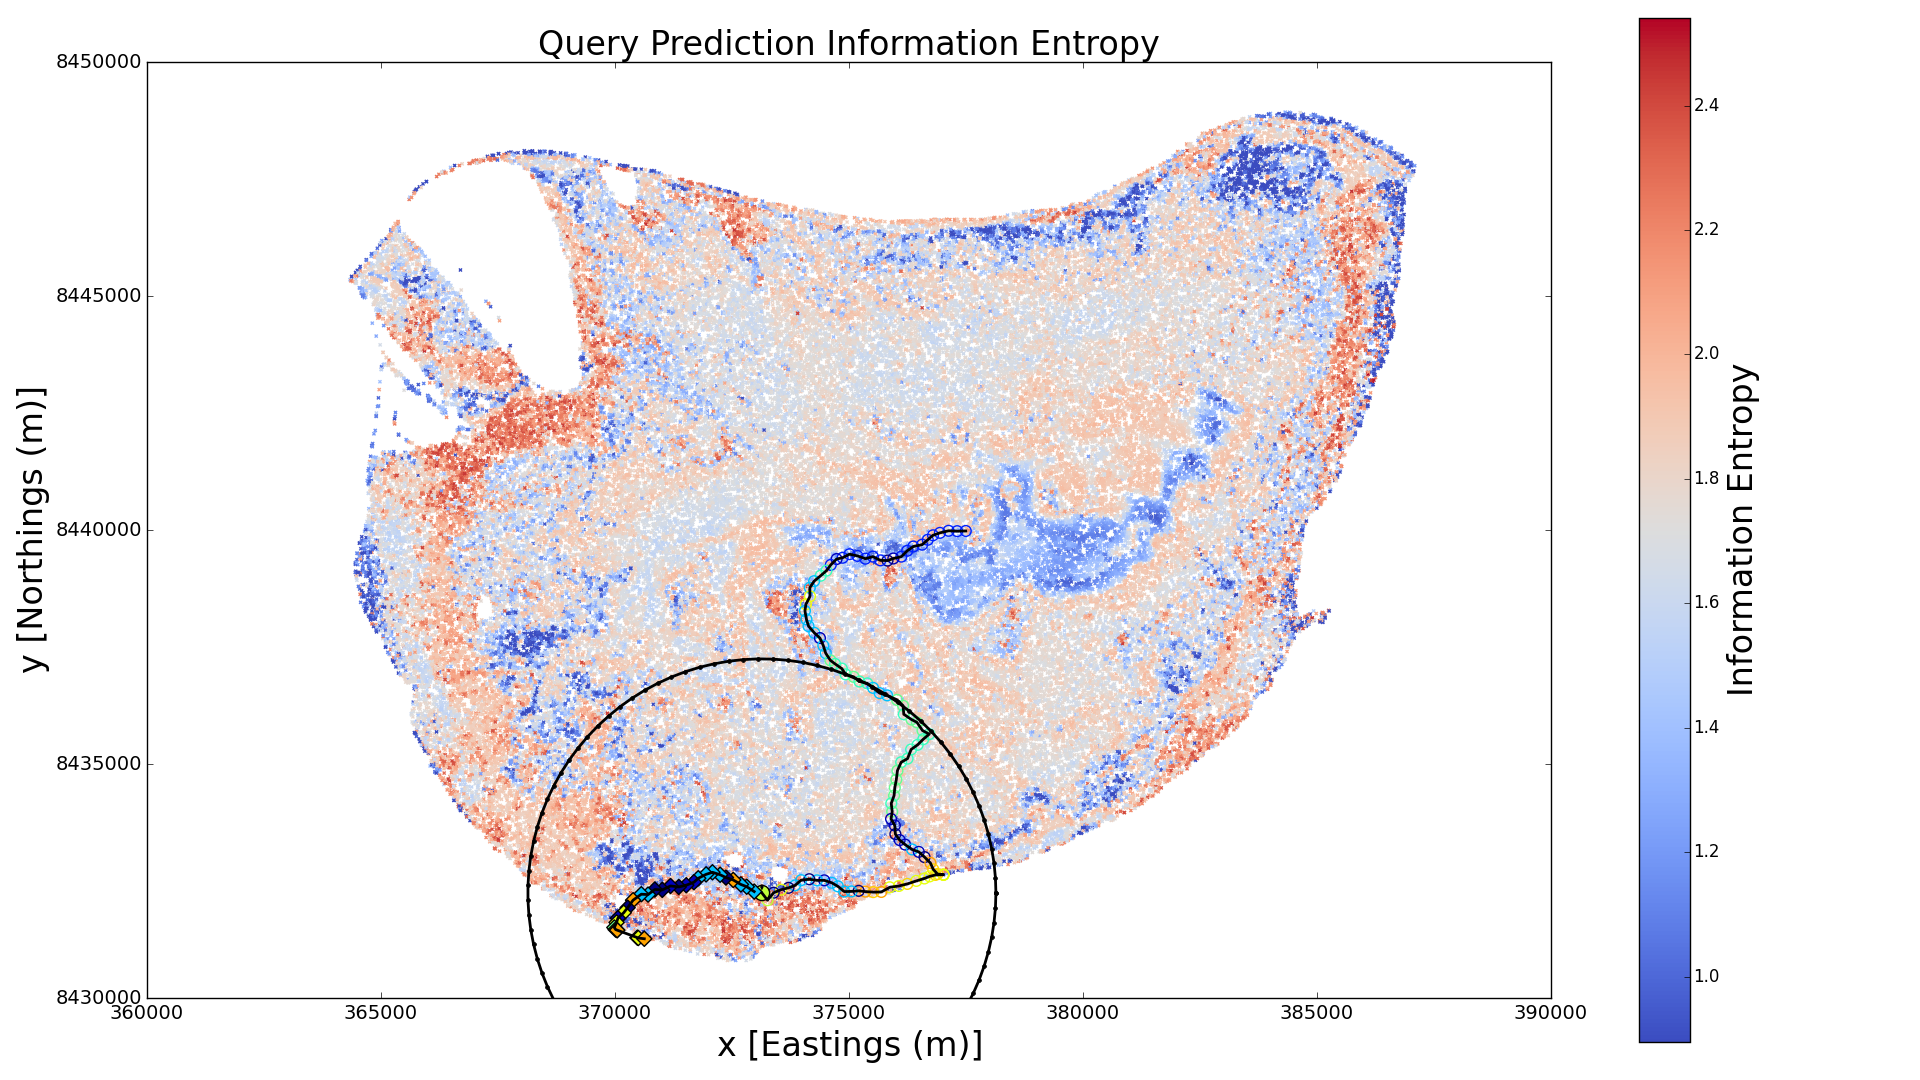
\includegraphics[width = 0.24\linewidth]{Figures/location_1_mcje_path/mie_propose_step100.png}
			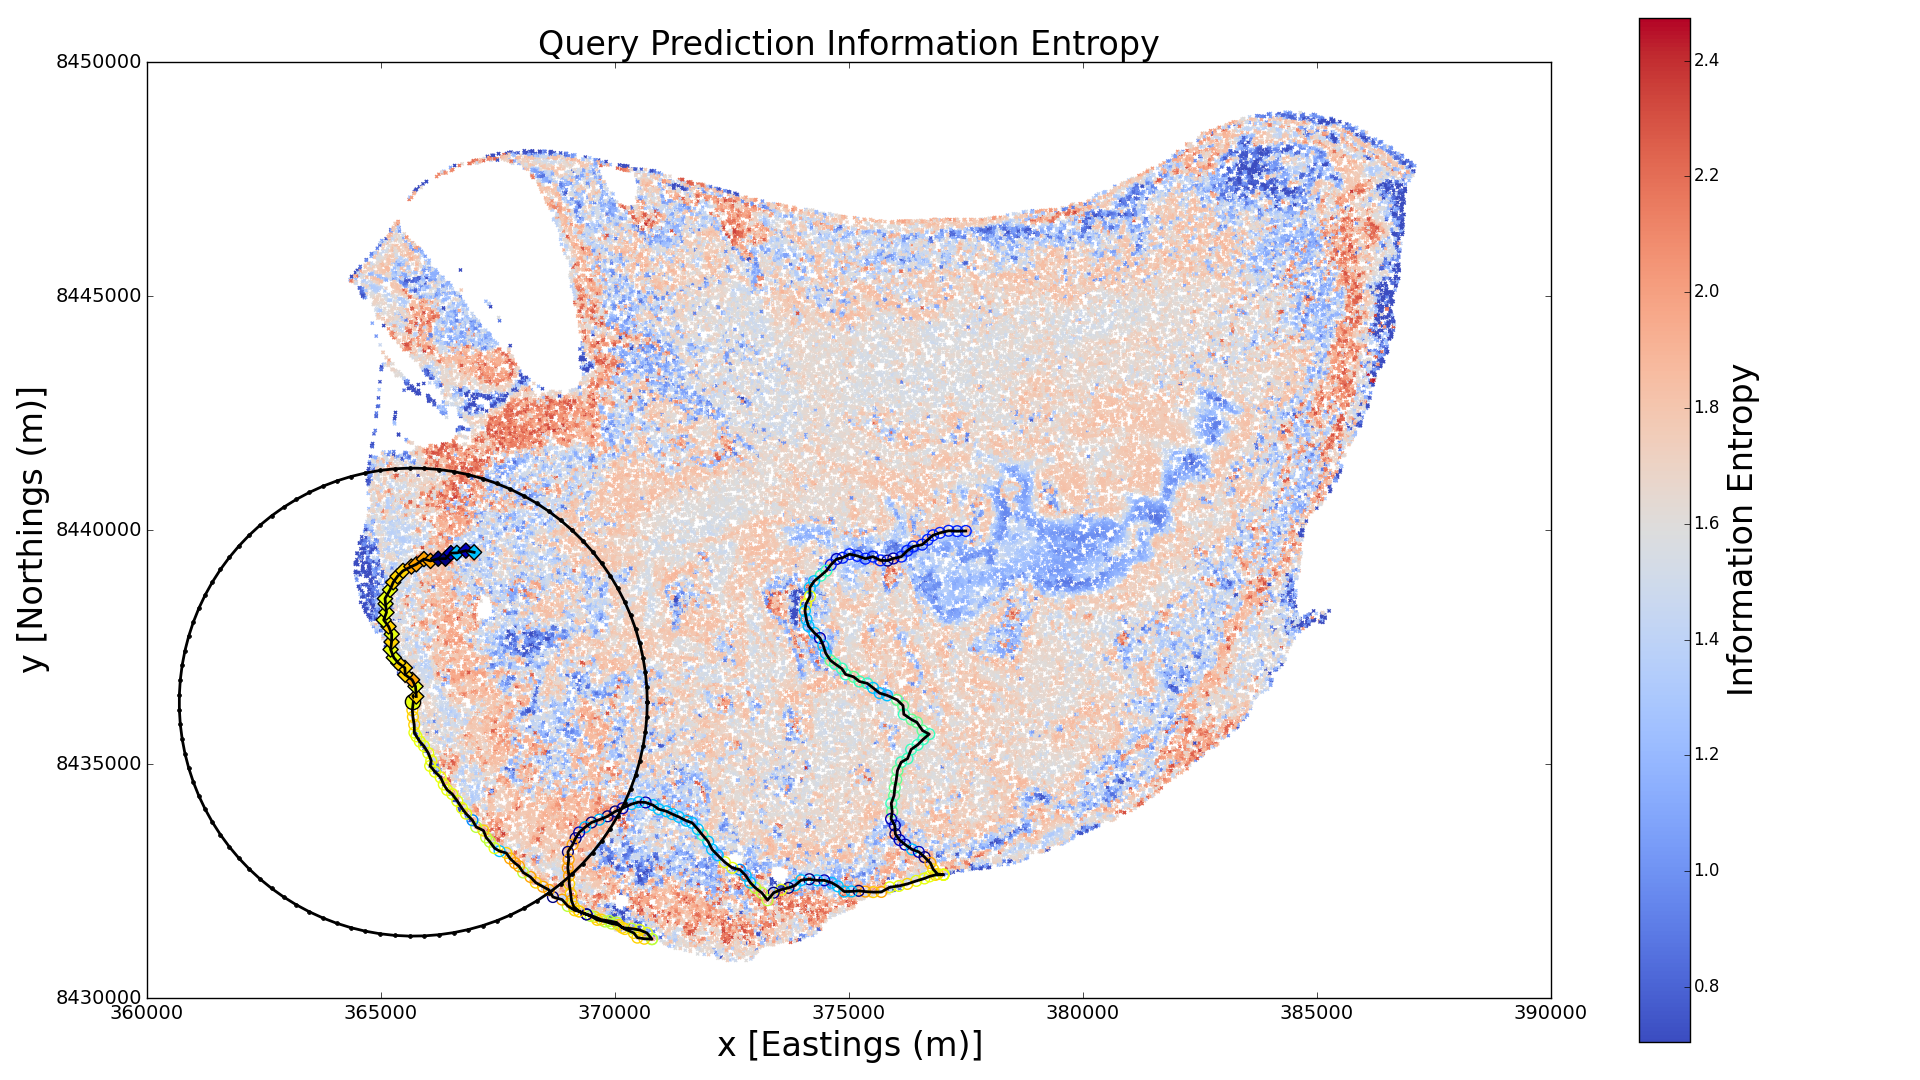
\includegraphics[width = 0.24\linewidth]{Figures/location_1_mcje_path/mie_propose_step200.png}
			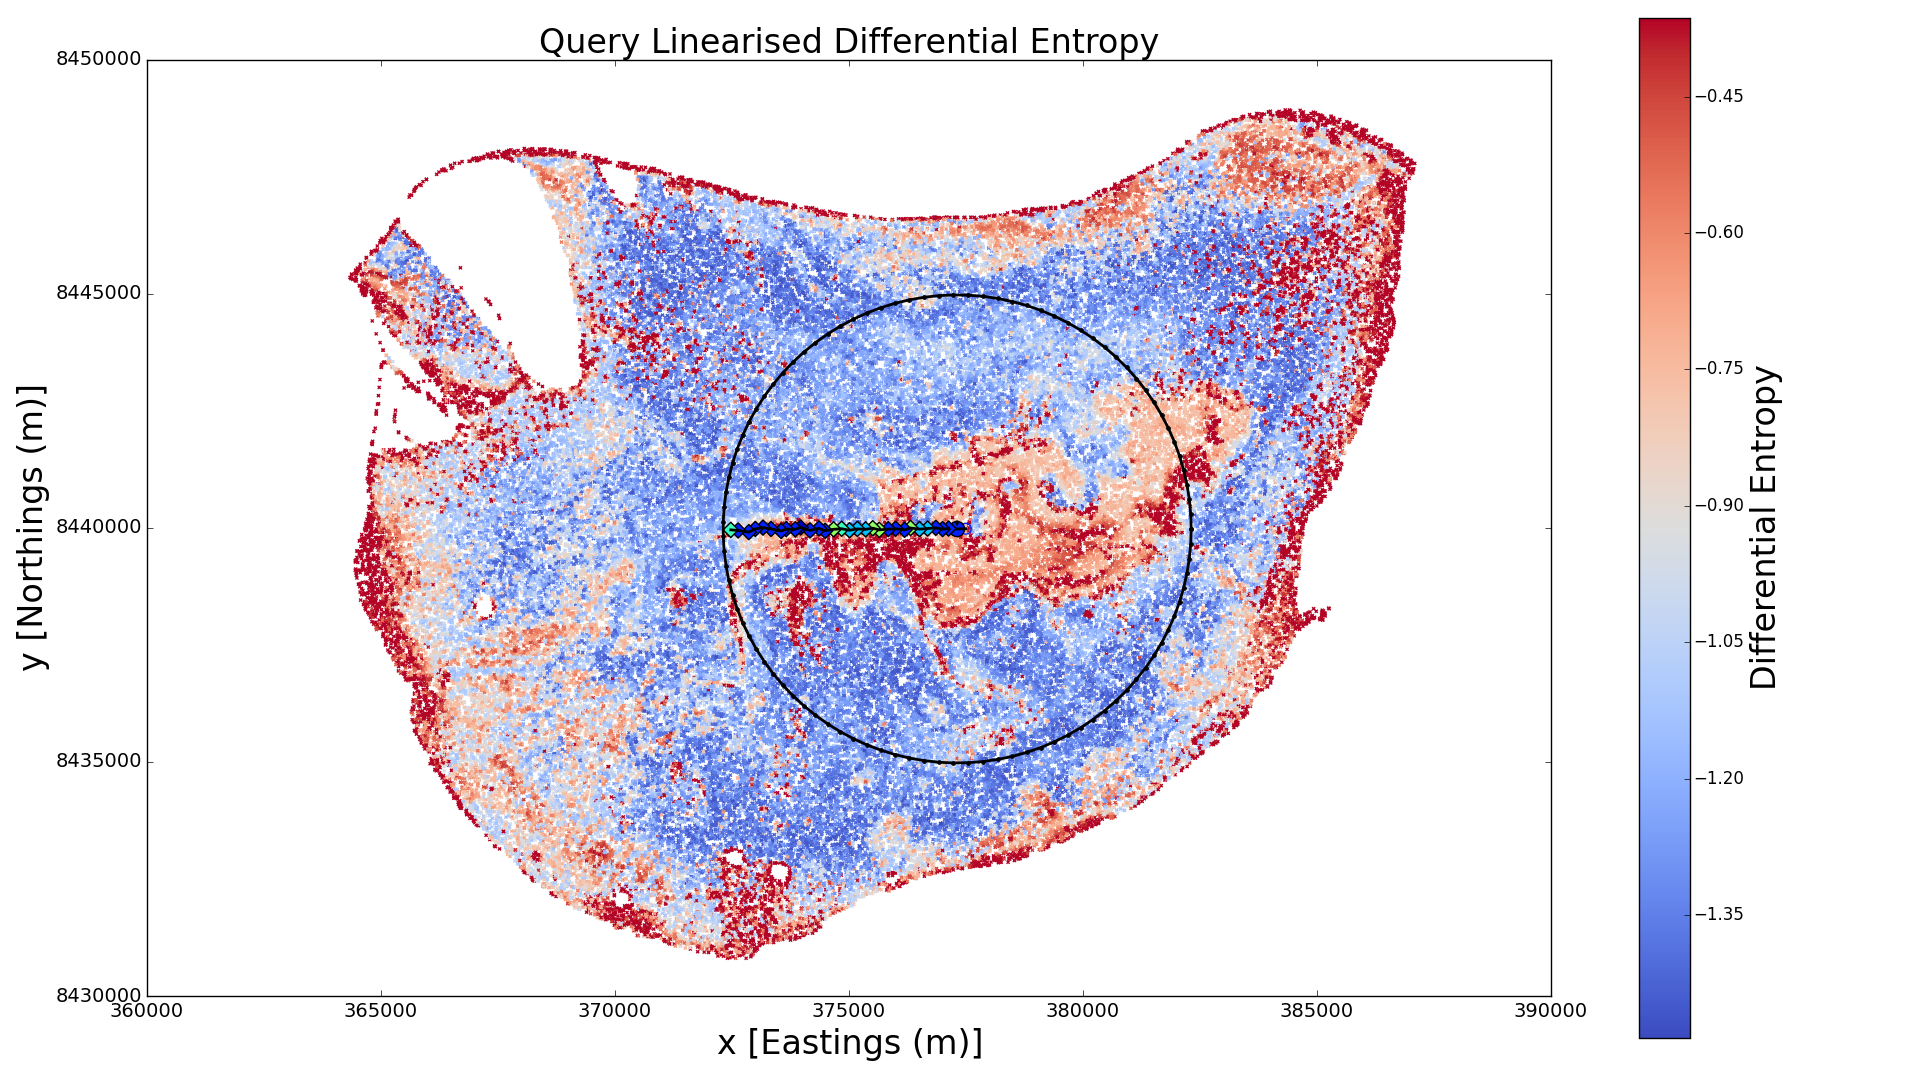
\includegraphics[width = 0.24\linewidth]{Figures/location_1_mcje_path/lde_propose_step1.png}
			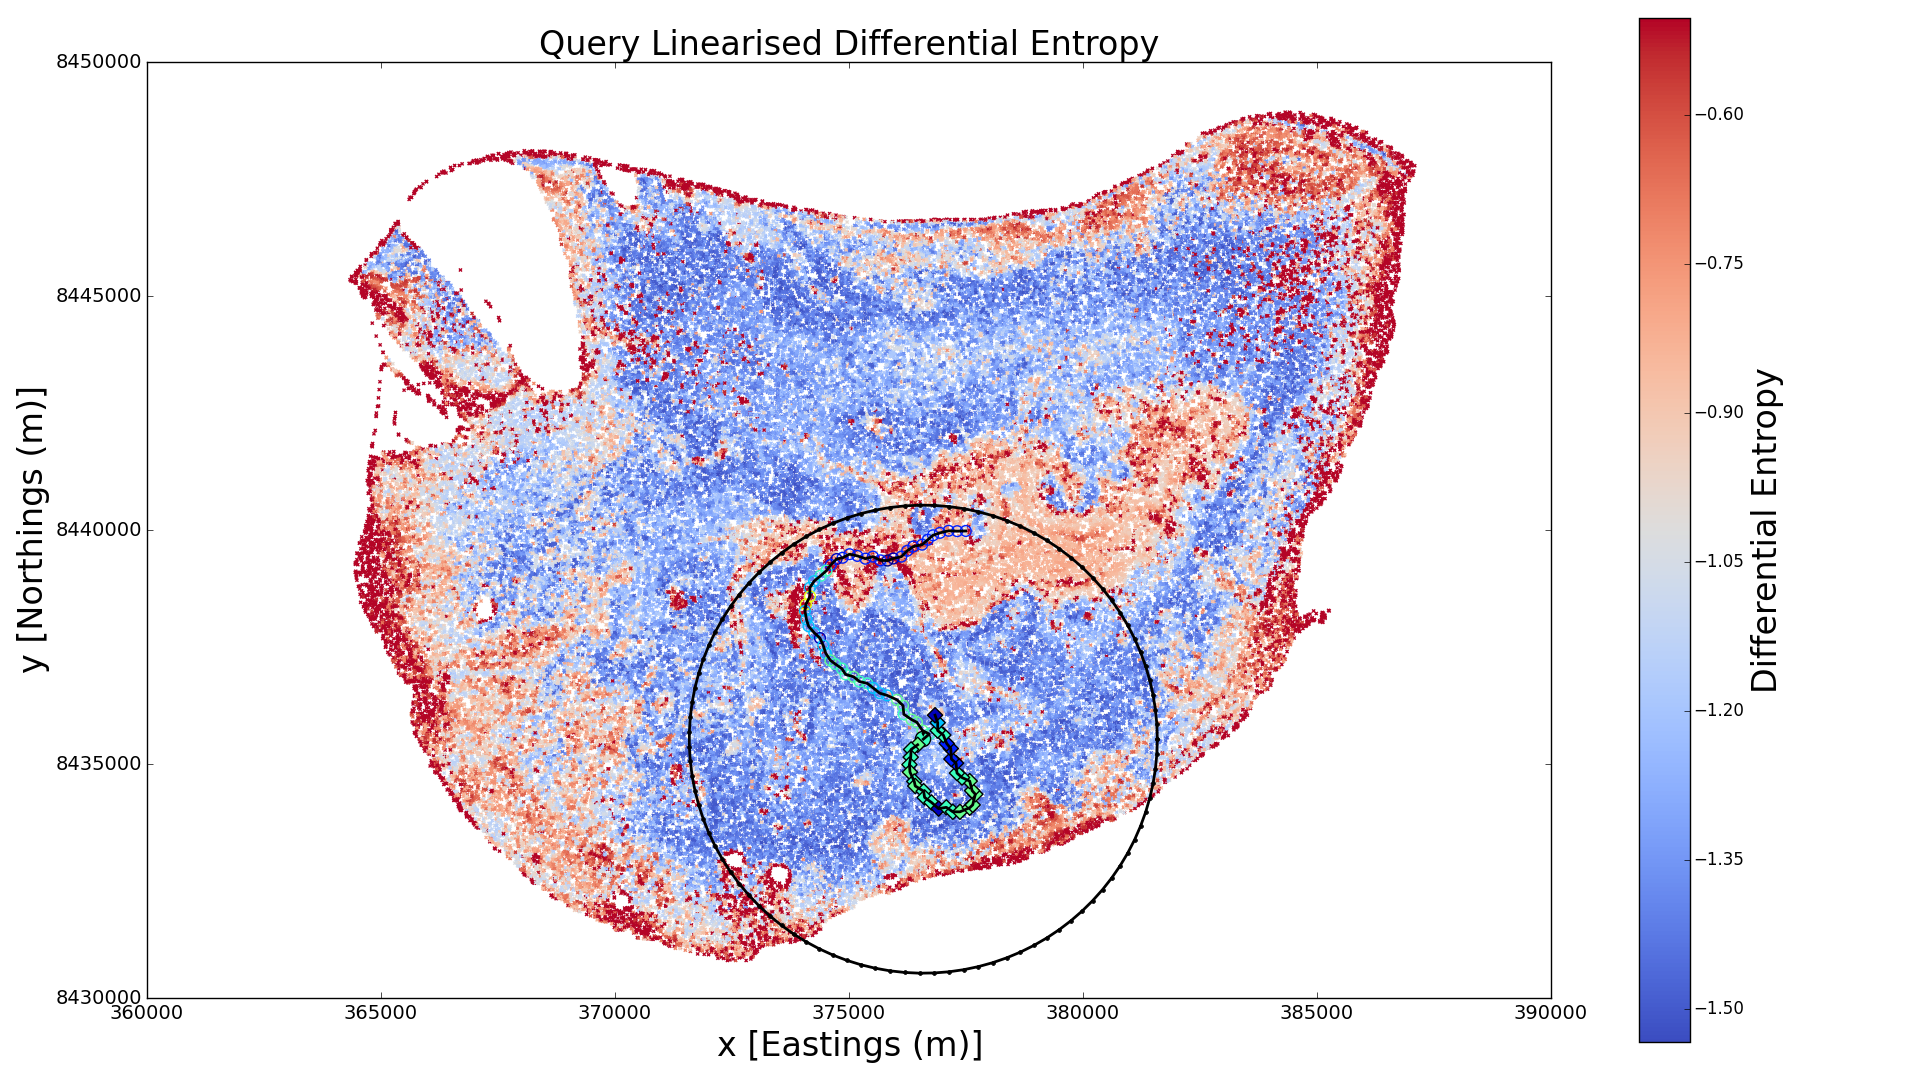
\includegraphics[width = 0.24\linewidth]{Figures/location_1_mcje_path/lde_propose_step50.png}
			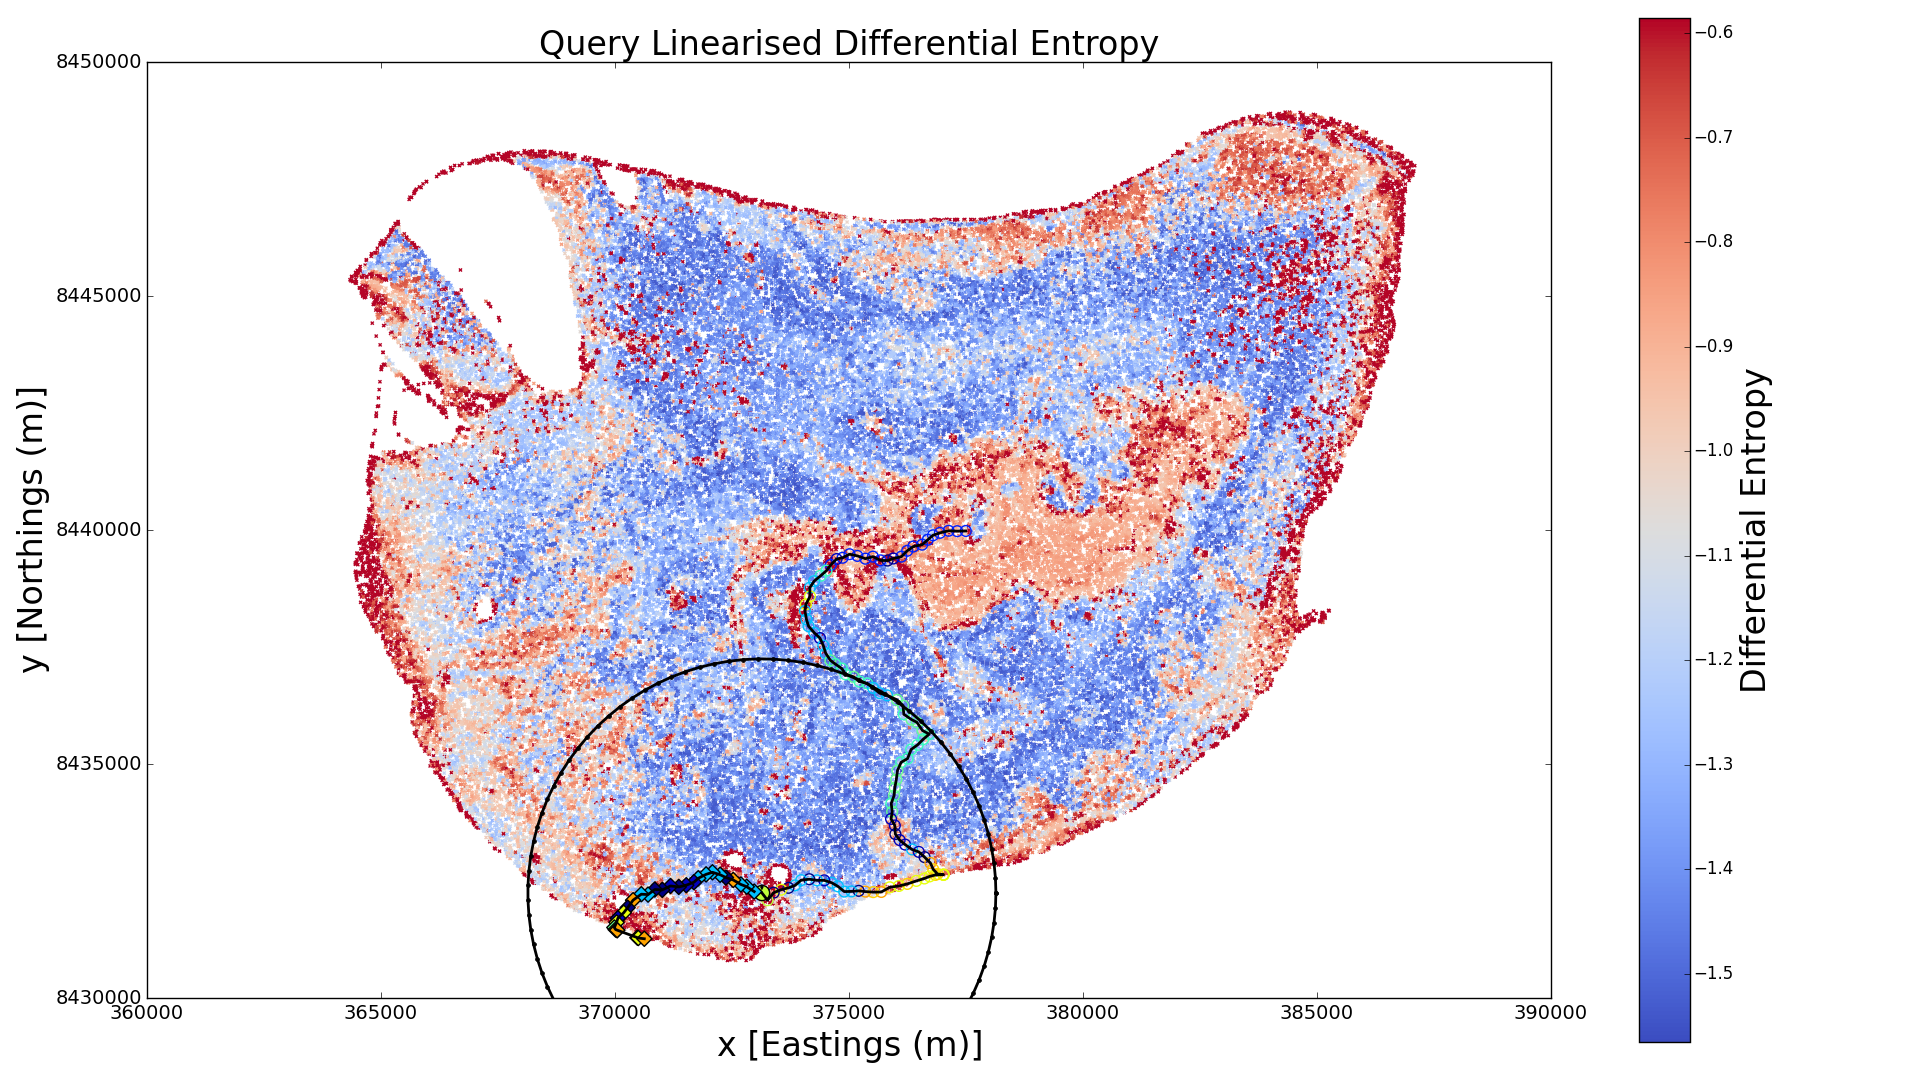
\includegraphics[width = 0.24\linewidth]{Figures/location_1_mcje_path/lde_propose_step100.png}
			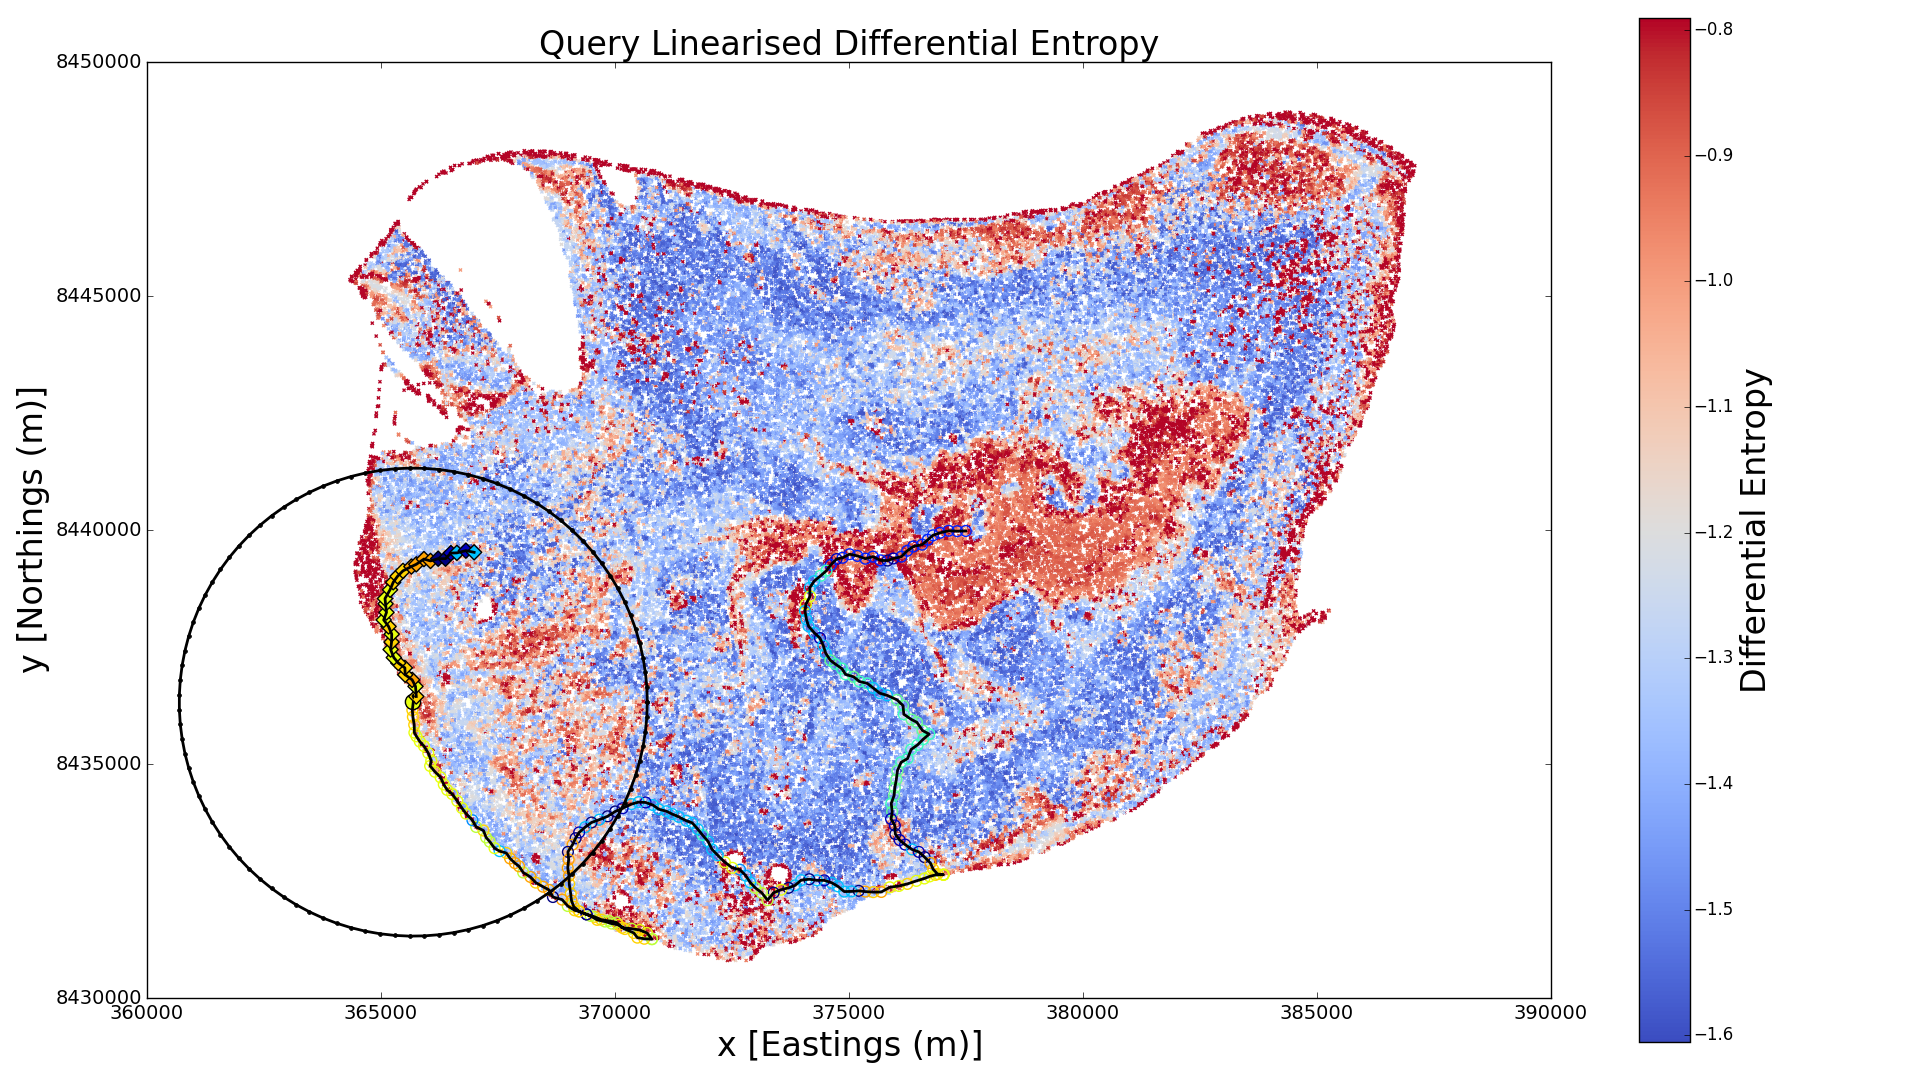
\includegraphics[width = 0.24\linewidth]{Figures/location_1_mcje_path/lde_propose_step200.png}
			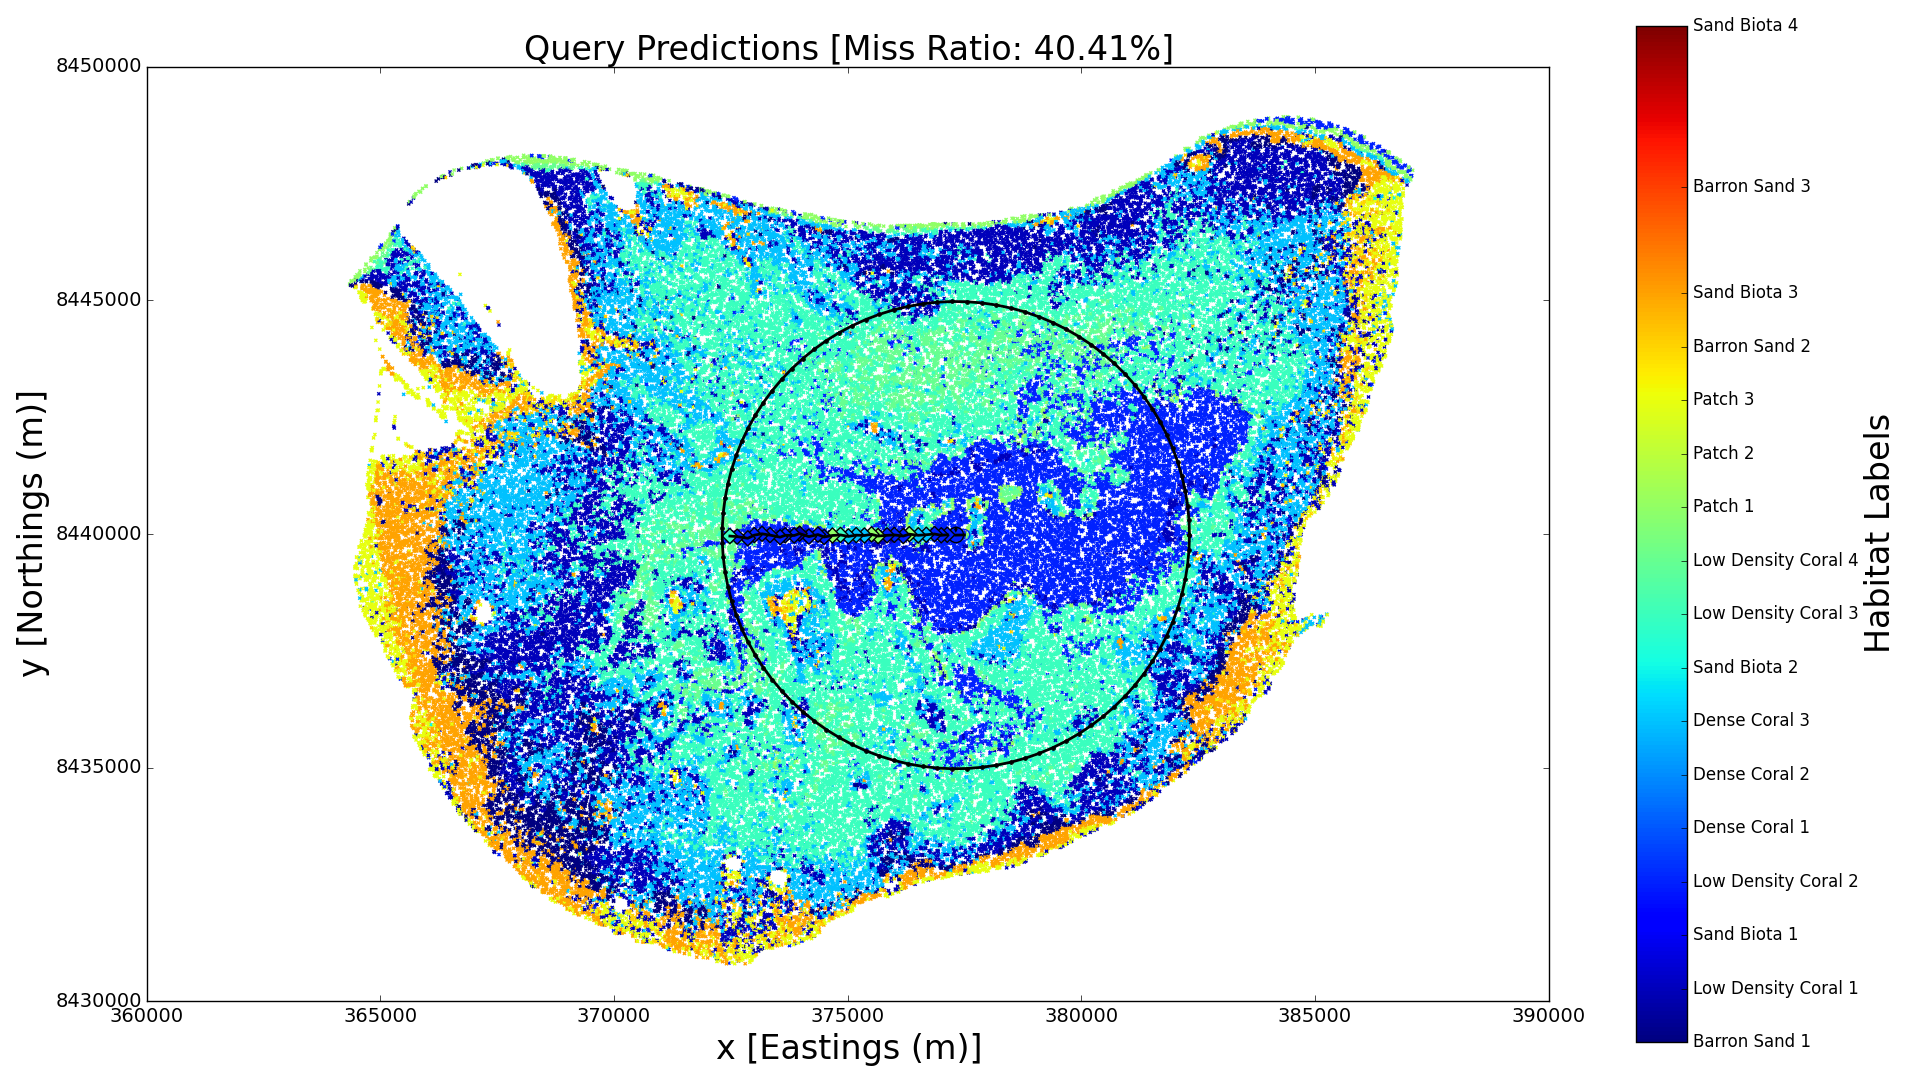
\includegraphics[width = 0.24\linewidth]{Figures/location_1_mcje_path/pred_propose_step1.png}
			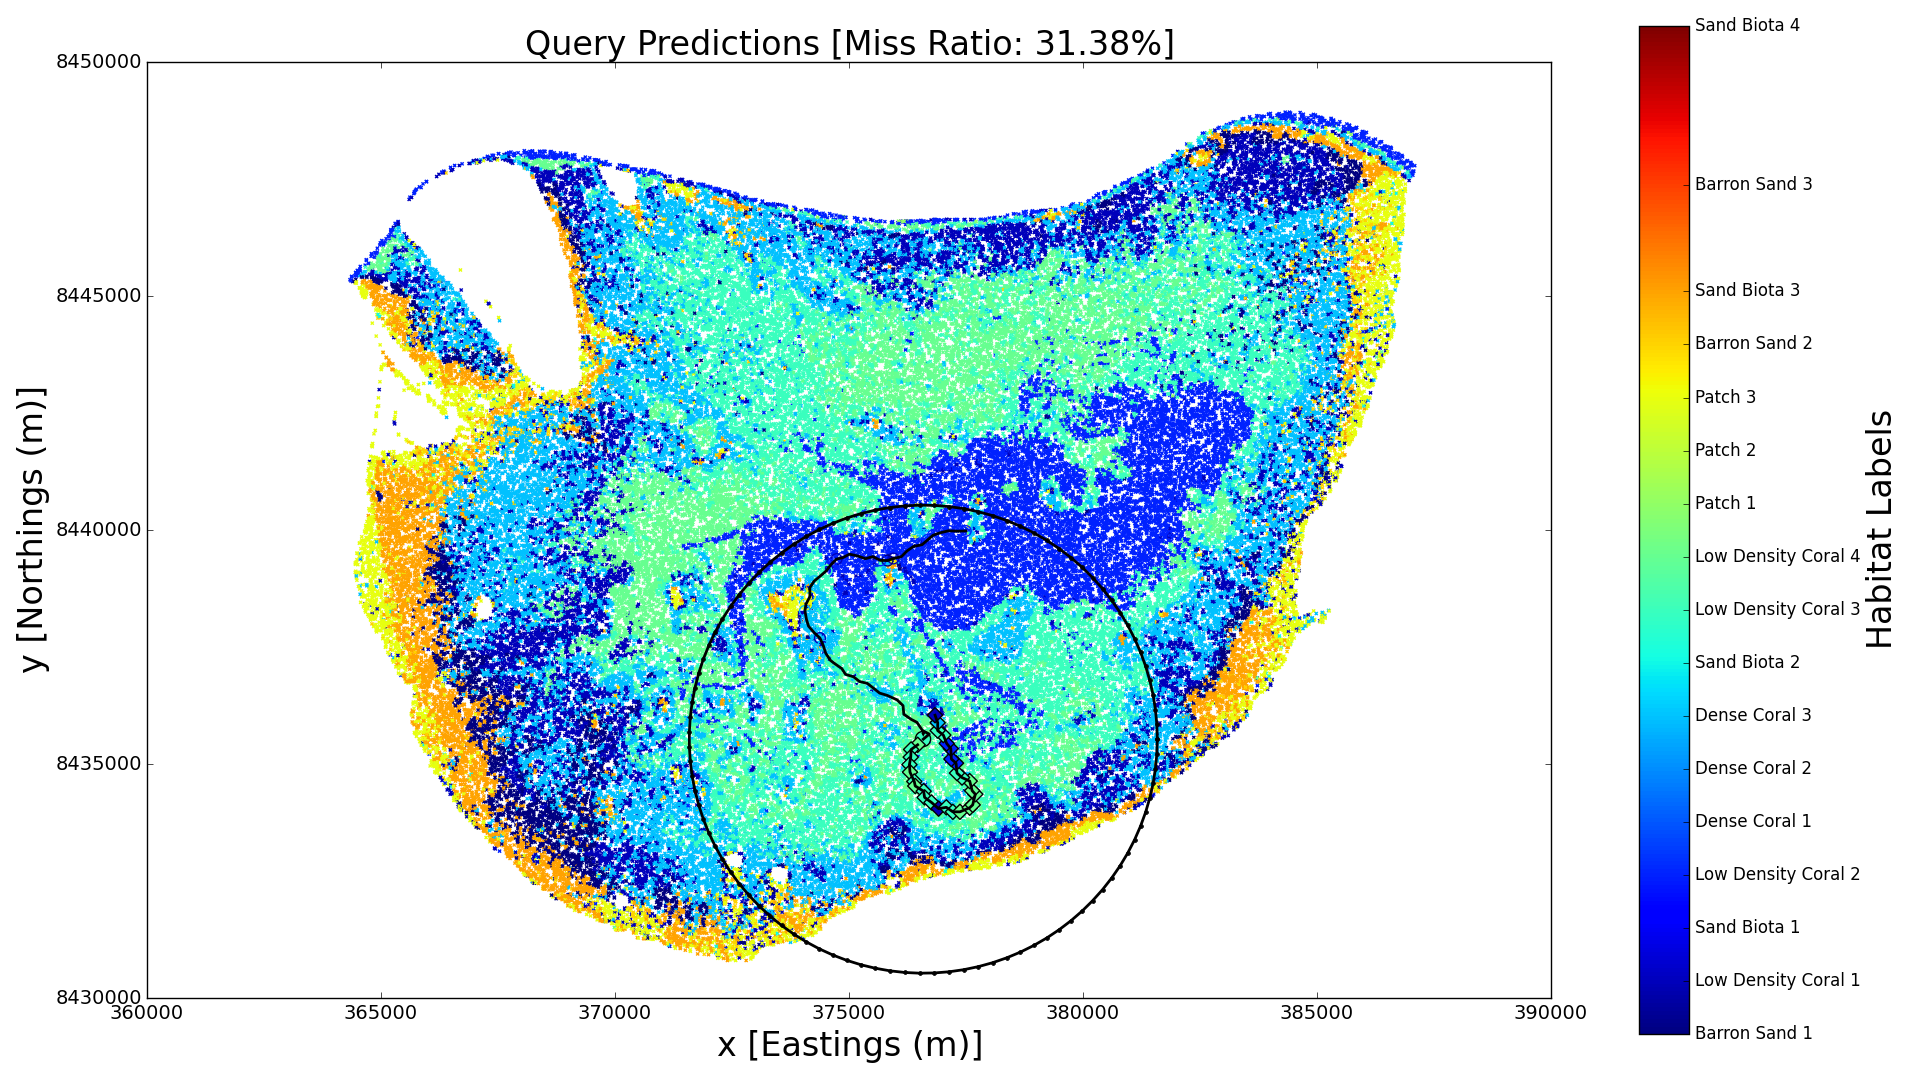
\includegraphics[width = 0.24\linewidth]{Figures/location_1_mcje_path/pred_propose_step50.png}
			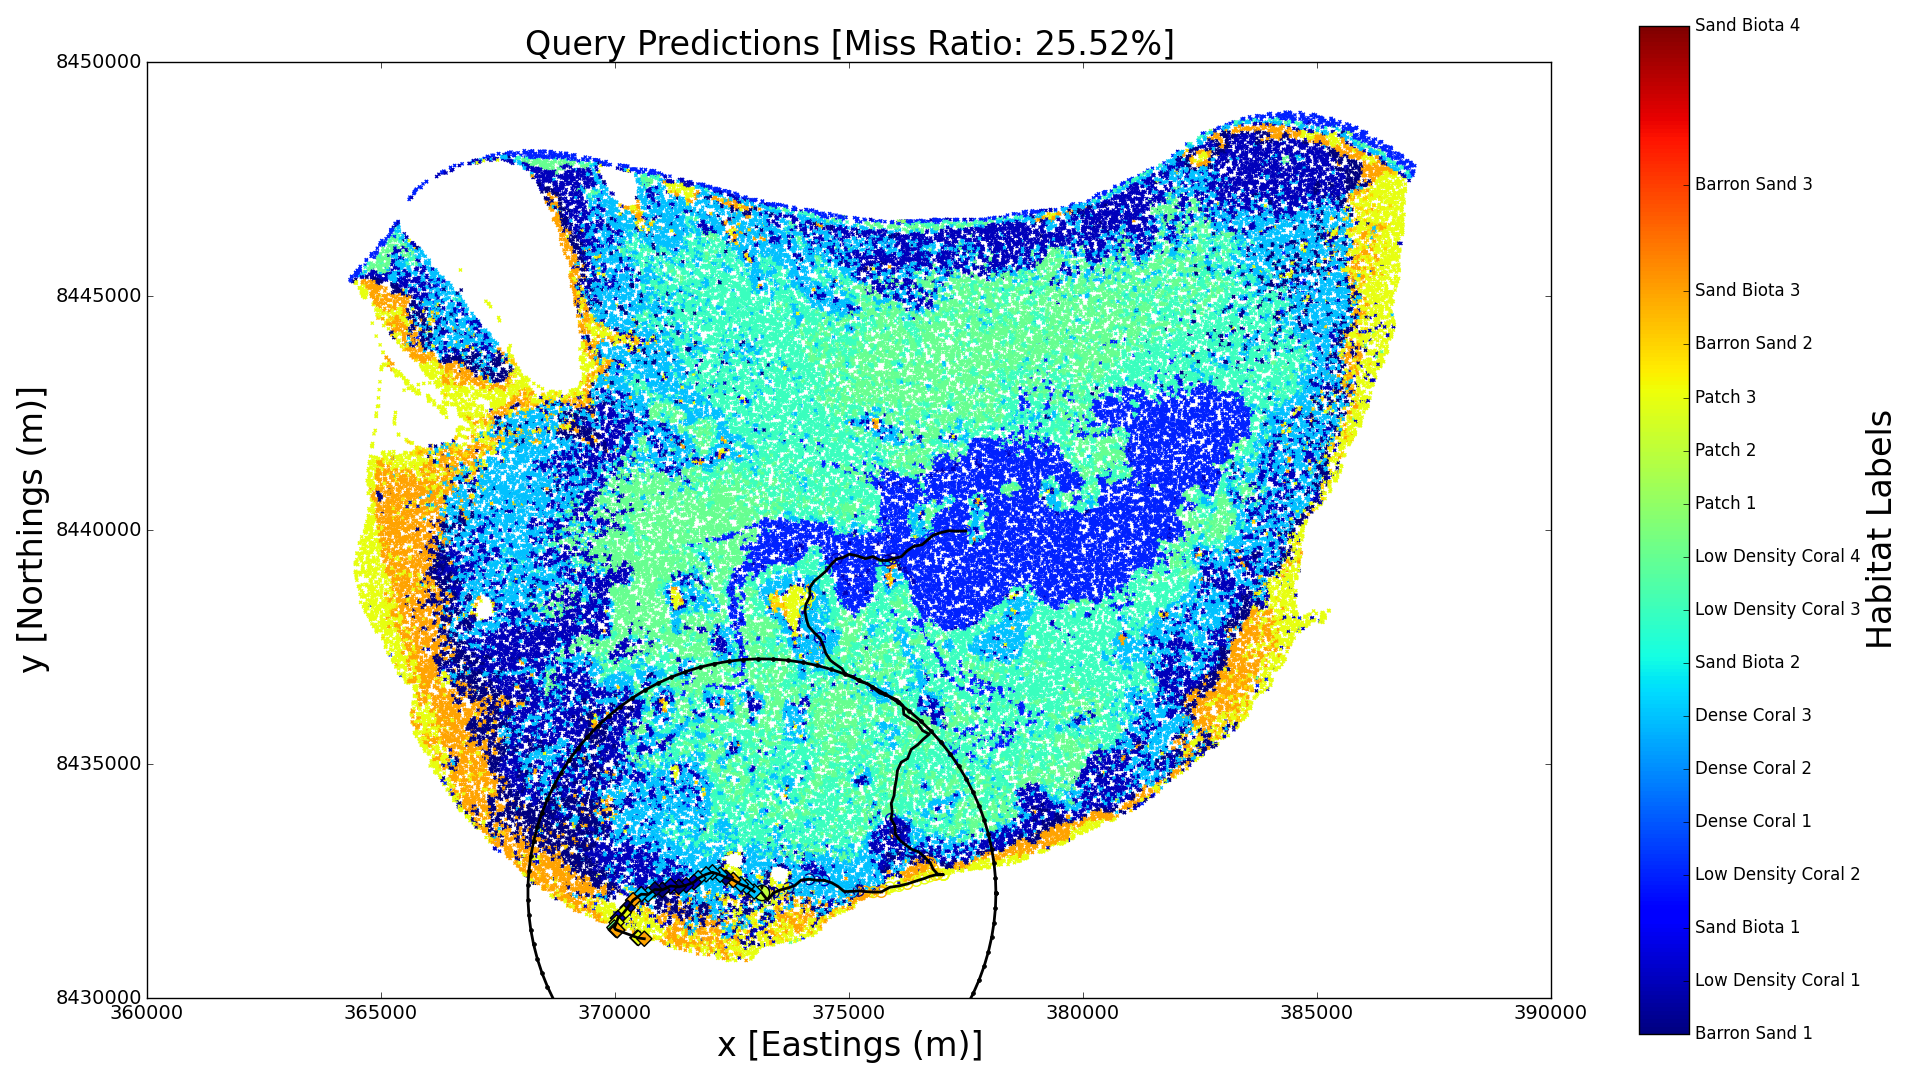
\includegraphics[width = 0.24\linewidth]{Figures/location_1_mcje_path/pred_propose_step100.png}
			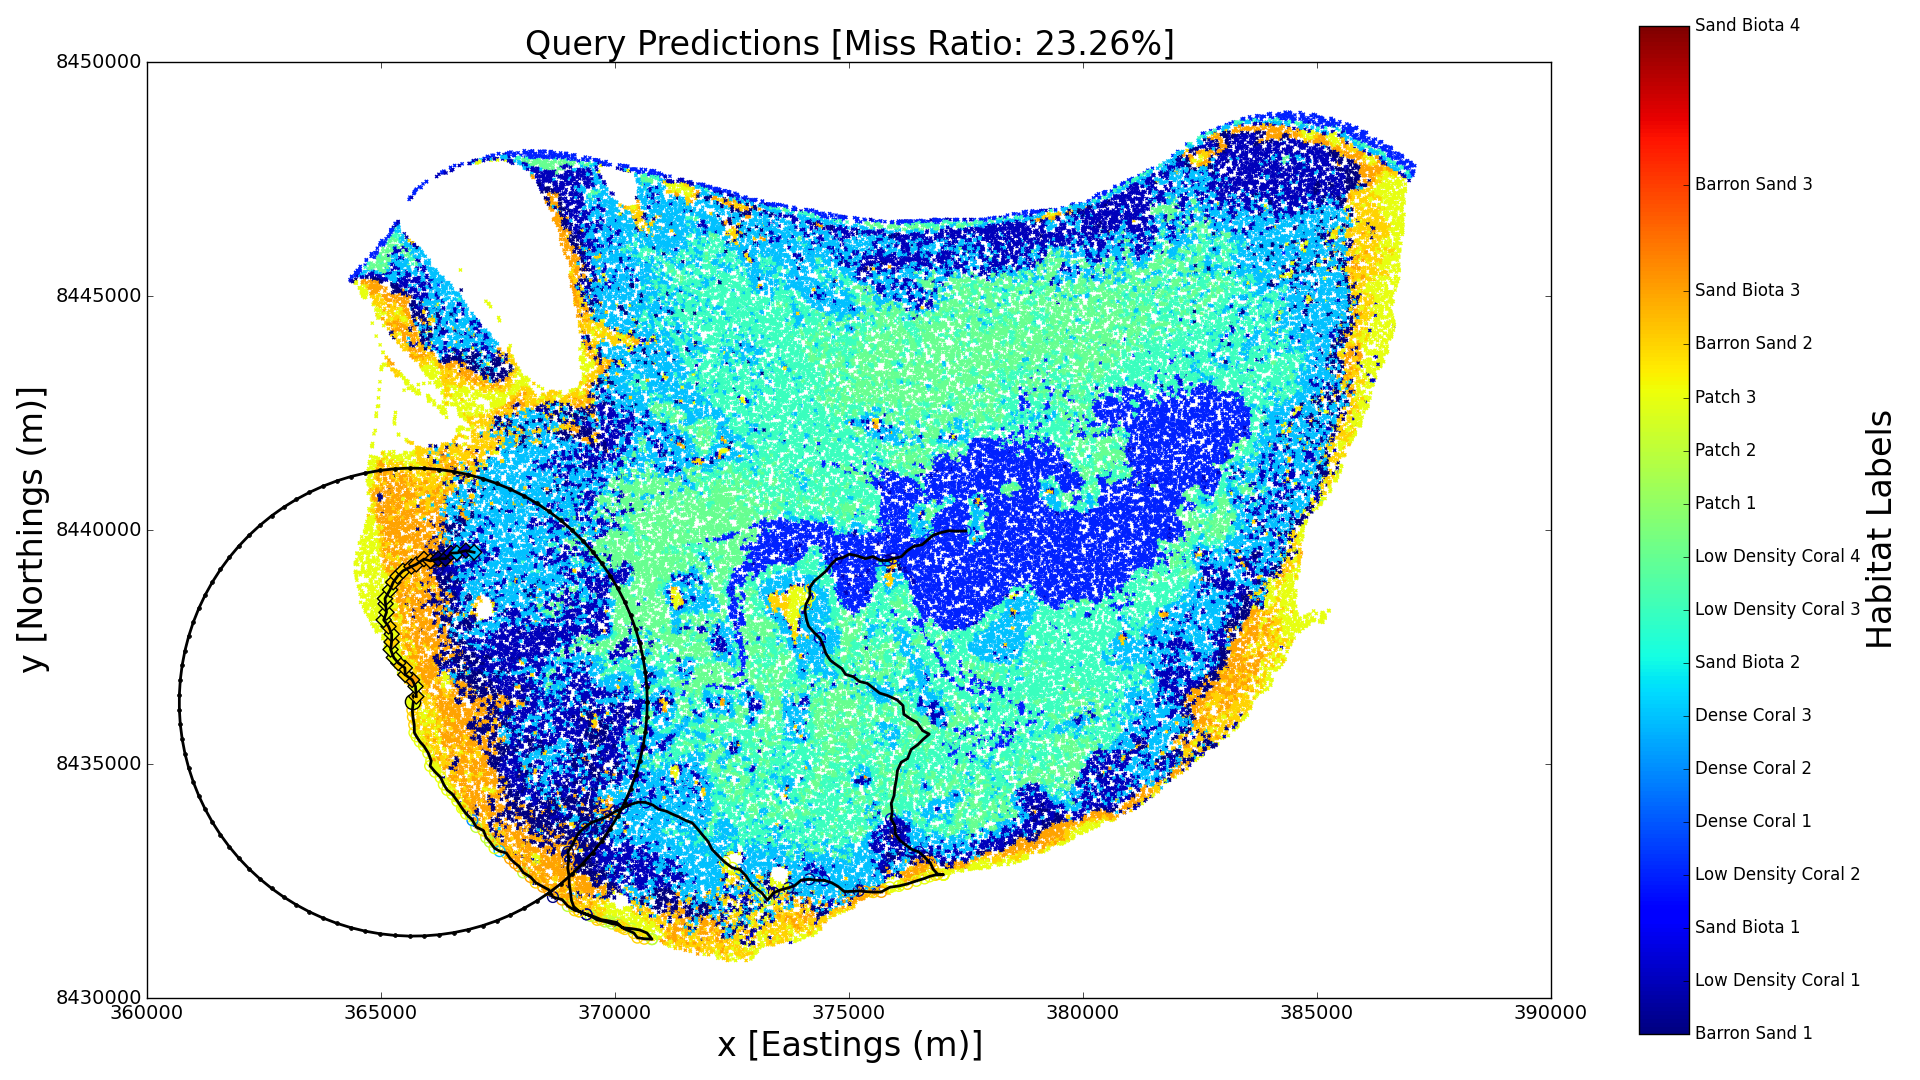
\includegraphics[width = 0.24\linewidth]{Figures/location_1_mcje_path/pred_propose_step200.png}			
		\caption{Exploration path under Monte Carlo estimated joint information entropy acquisition}
		\label{Figure:Results:OptimalPathMCJE}
		\end{figure*}
		
		A comparison in performance over a distance of 33.3 km between several acquisition criterion are shown in figure \ref{Figure:Results:CompareMethods}. Each method is tested with a horizon length of 5 km starting at two distinct initial locations. The acquisition criterion to be compared are linearised differential entropy (LDE), one step ahead information entropy (GREEDY), random walk (RANDOM), Monte Carlo estimated joint information entropy (MCJIE), sum of marginalised information entropy (MIE), predetermined spiral path (FIXED-SPIRAL), and predetermined line segmented paths (FIXED-LINES).
	
		\begin{figure}[!htbp]
		\centering
			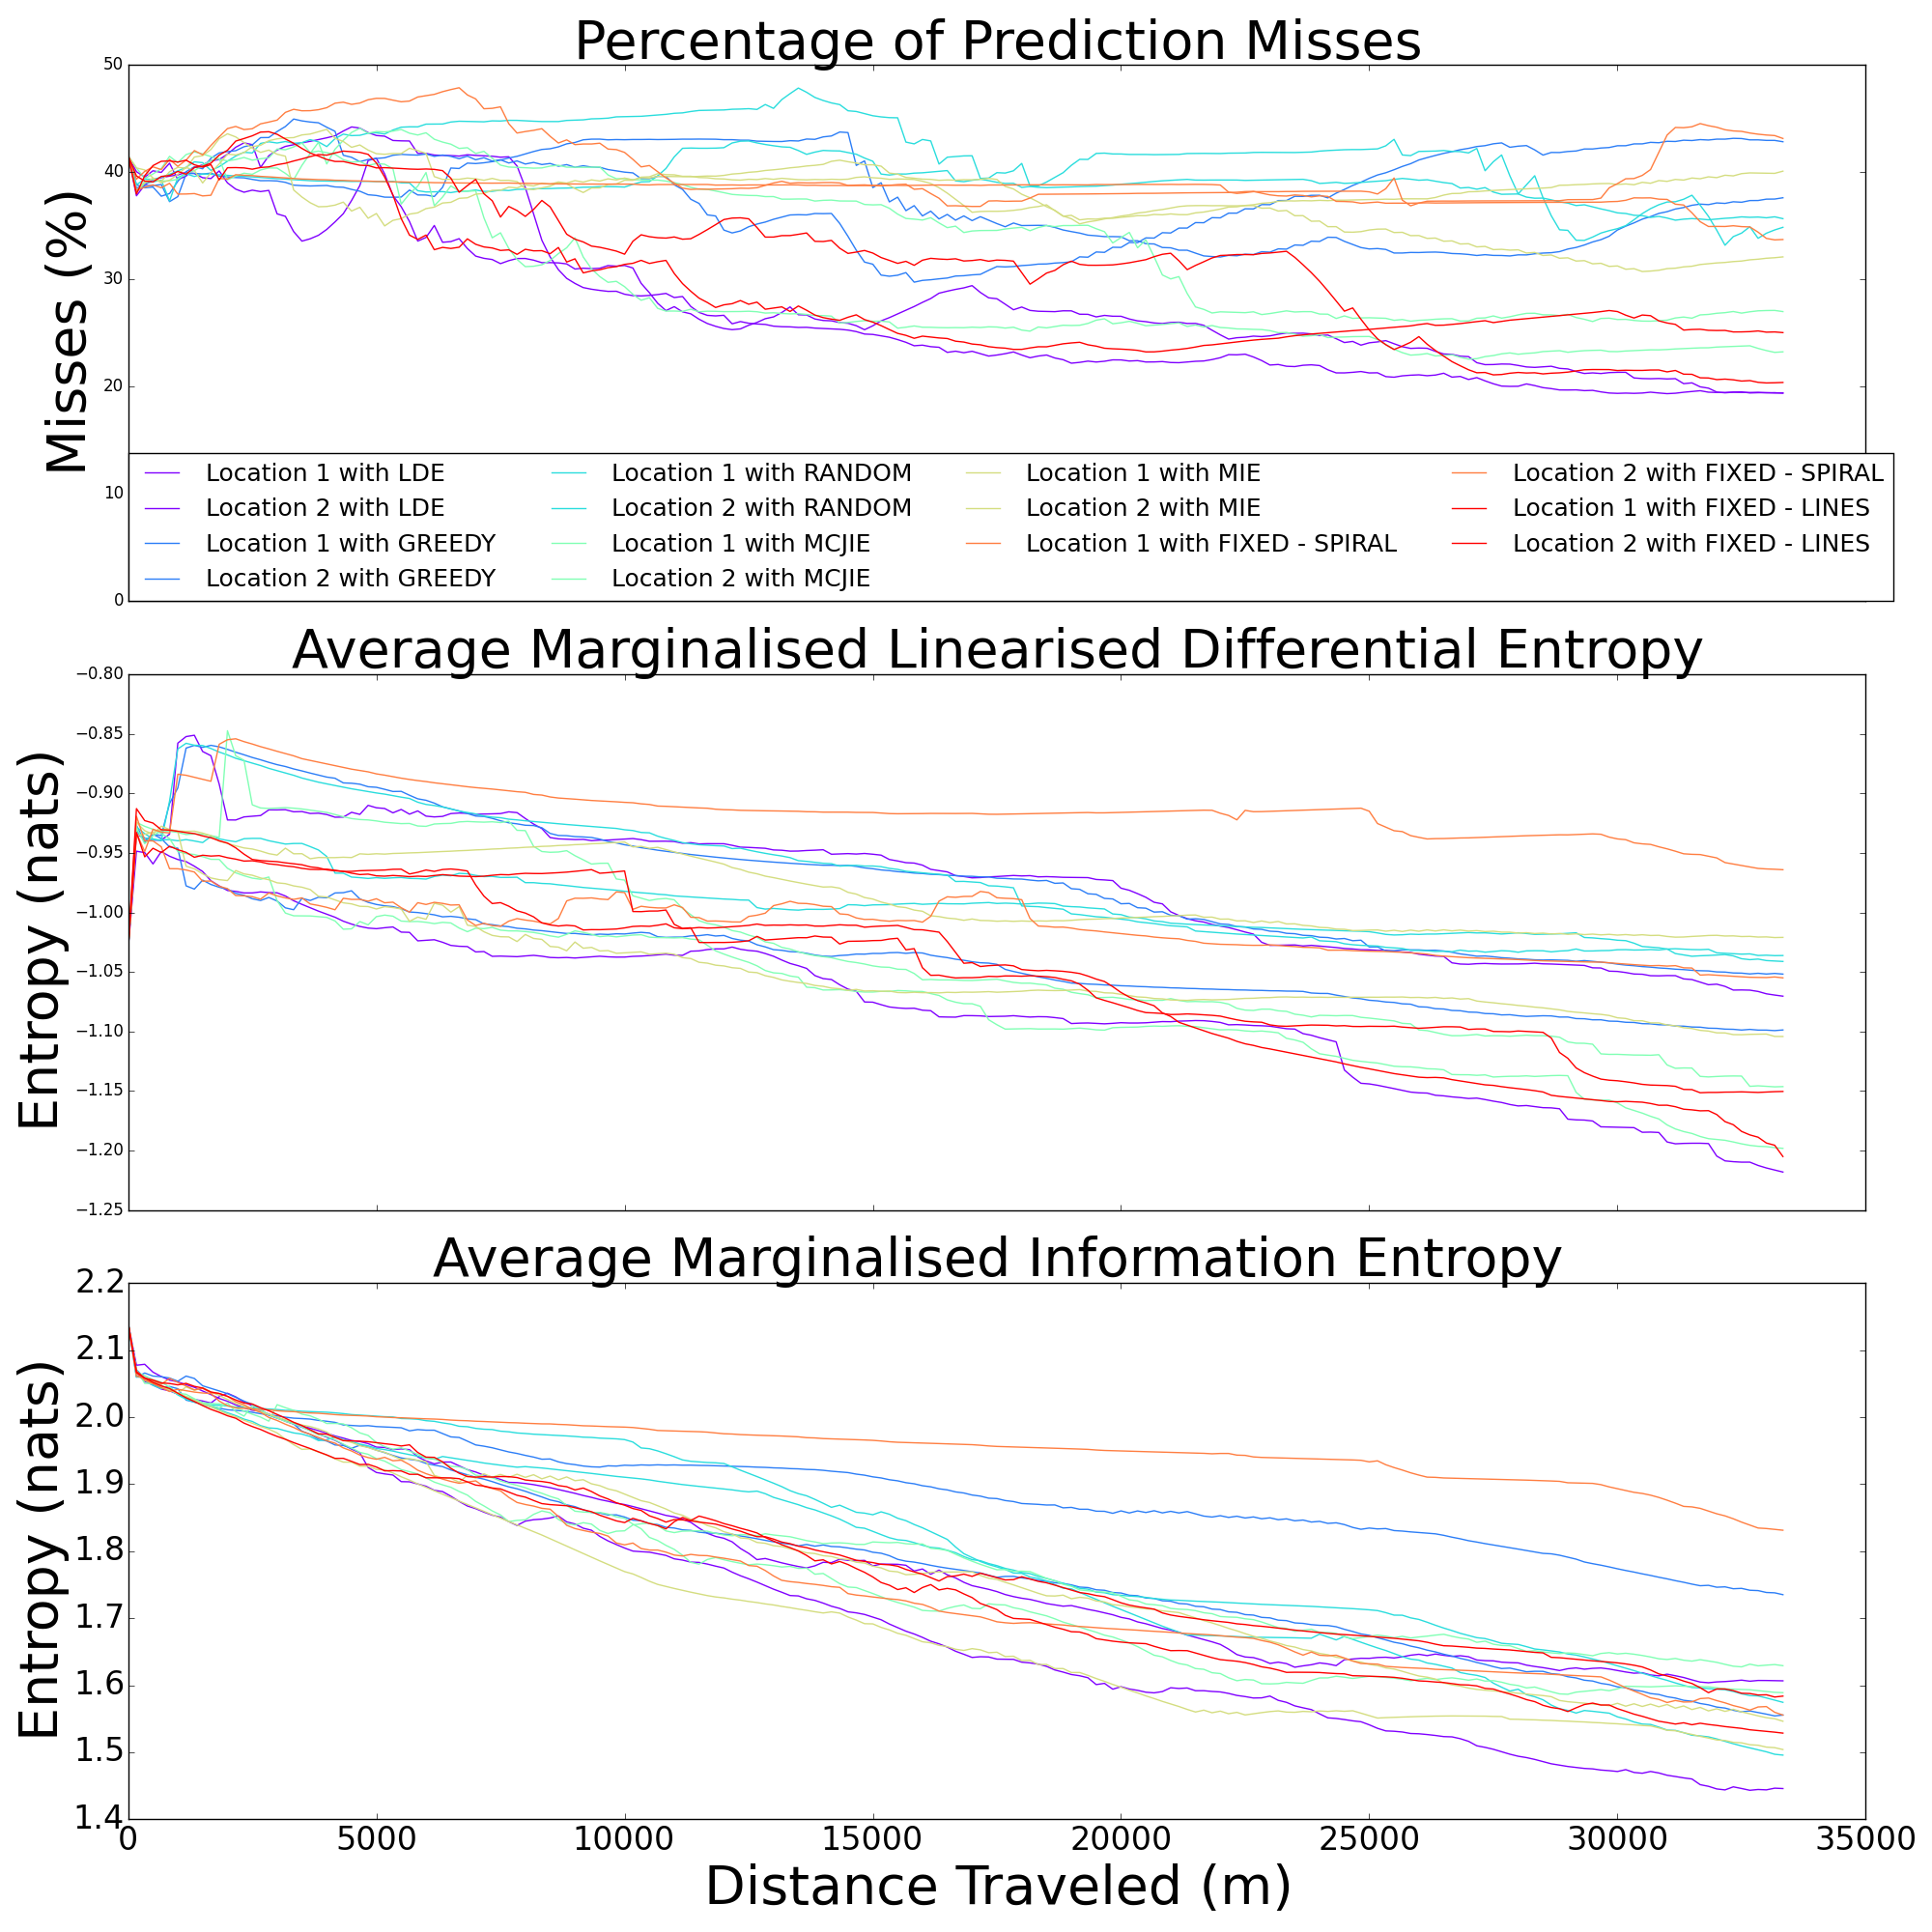
\includegraphics[width = \linewidth]{Figures/compare_methods.png}
		\caption{Horizon Effects}
		\label{Figure:Results:CompareMethods}
		\end{figure}
			
		There are several measures of performance criterion that can be used to measure performance. As the aim is to reduce misclassification rate, we compare the percentage of prediction misses between each method. Each method begins with the same scenario, for which the initial misclassification rate with 200 training points is 41.54\% (figure \ref{Figure:Results:ScottReefInitialPredictions}). From figure \ref{Figure:Results:CompareMethods}, we see that under this performance criterion, the LDE method performs the best, with a final misclassification rate of 19.43\% and 19.40\% for location 1 and 2 respectively at the end of the journey. Methods FIXED-LINES (20.40\% and 25.05\%) and MCJIE (23.26\% and 27.01\%) follow in performance. The predetermined line segmented paths are hand-picked by subjective judgement from after-the-fact knowledge, and serve as an intuitive anchor for comparison. Notice that because the LDE method prioritises on decision boundaries, it achieves a lower misclassification rate through appropriately reducing the entropy at decision boundaries.
			
%----------
%('Location 1 with LDE', 0.19427)
%('Location 1 with FIXED - LINES', 0.20402000000000001)
%('Location 1 with MCJIE', 0.23258000000000001)
%('Location 1 with MIE', 0.32114999999999999)
%('Location 1 with FIXED - SPIRAL', 0.33735999999999999)
%('Location 1 with RANDOM', 0.34873999999999999)
%('Location 1 with GREEDY', 0.42856)
%----------
%('Location 2 with LDE', 0.19402)
%('Location 2 with FIXED - LINES', 0.25052000000000002)
%('Location 2 with MCJIE', 0.27012000000000003)
%('Location 2 with RANDOM', 0.35681000000000002)
%('Location 2 with GREEDY', 0.37630000000000002)
%('Location 2 with MIE', 0.40111999999999998)
%('Location 2 with FIXED - SPIRAL', 0.43160999999999999)

		\begin{figure}[!htbp]
		\centering
			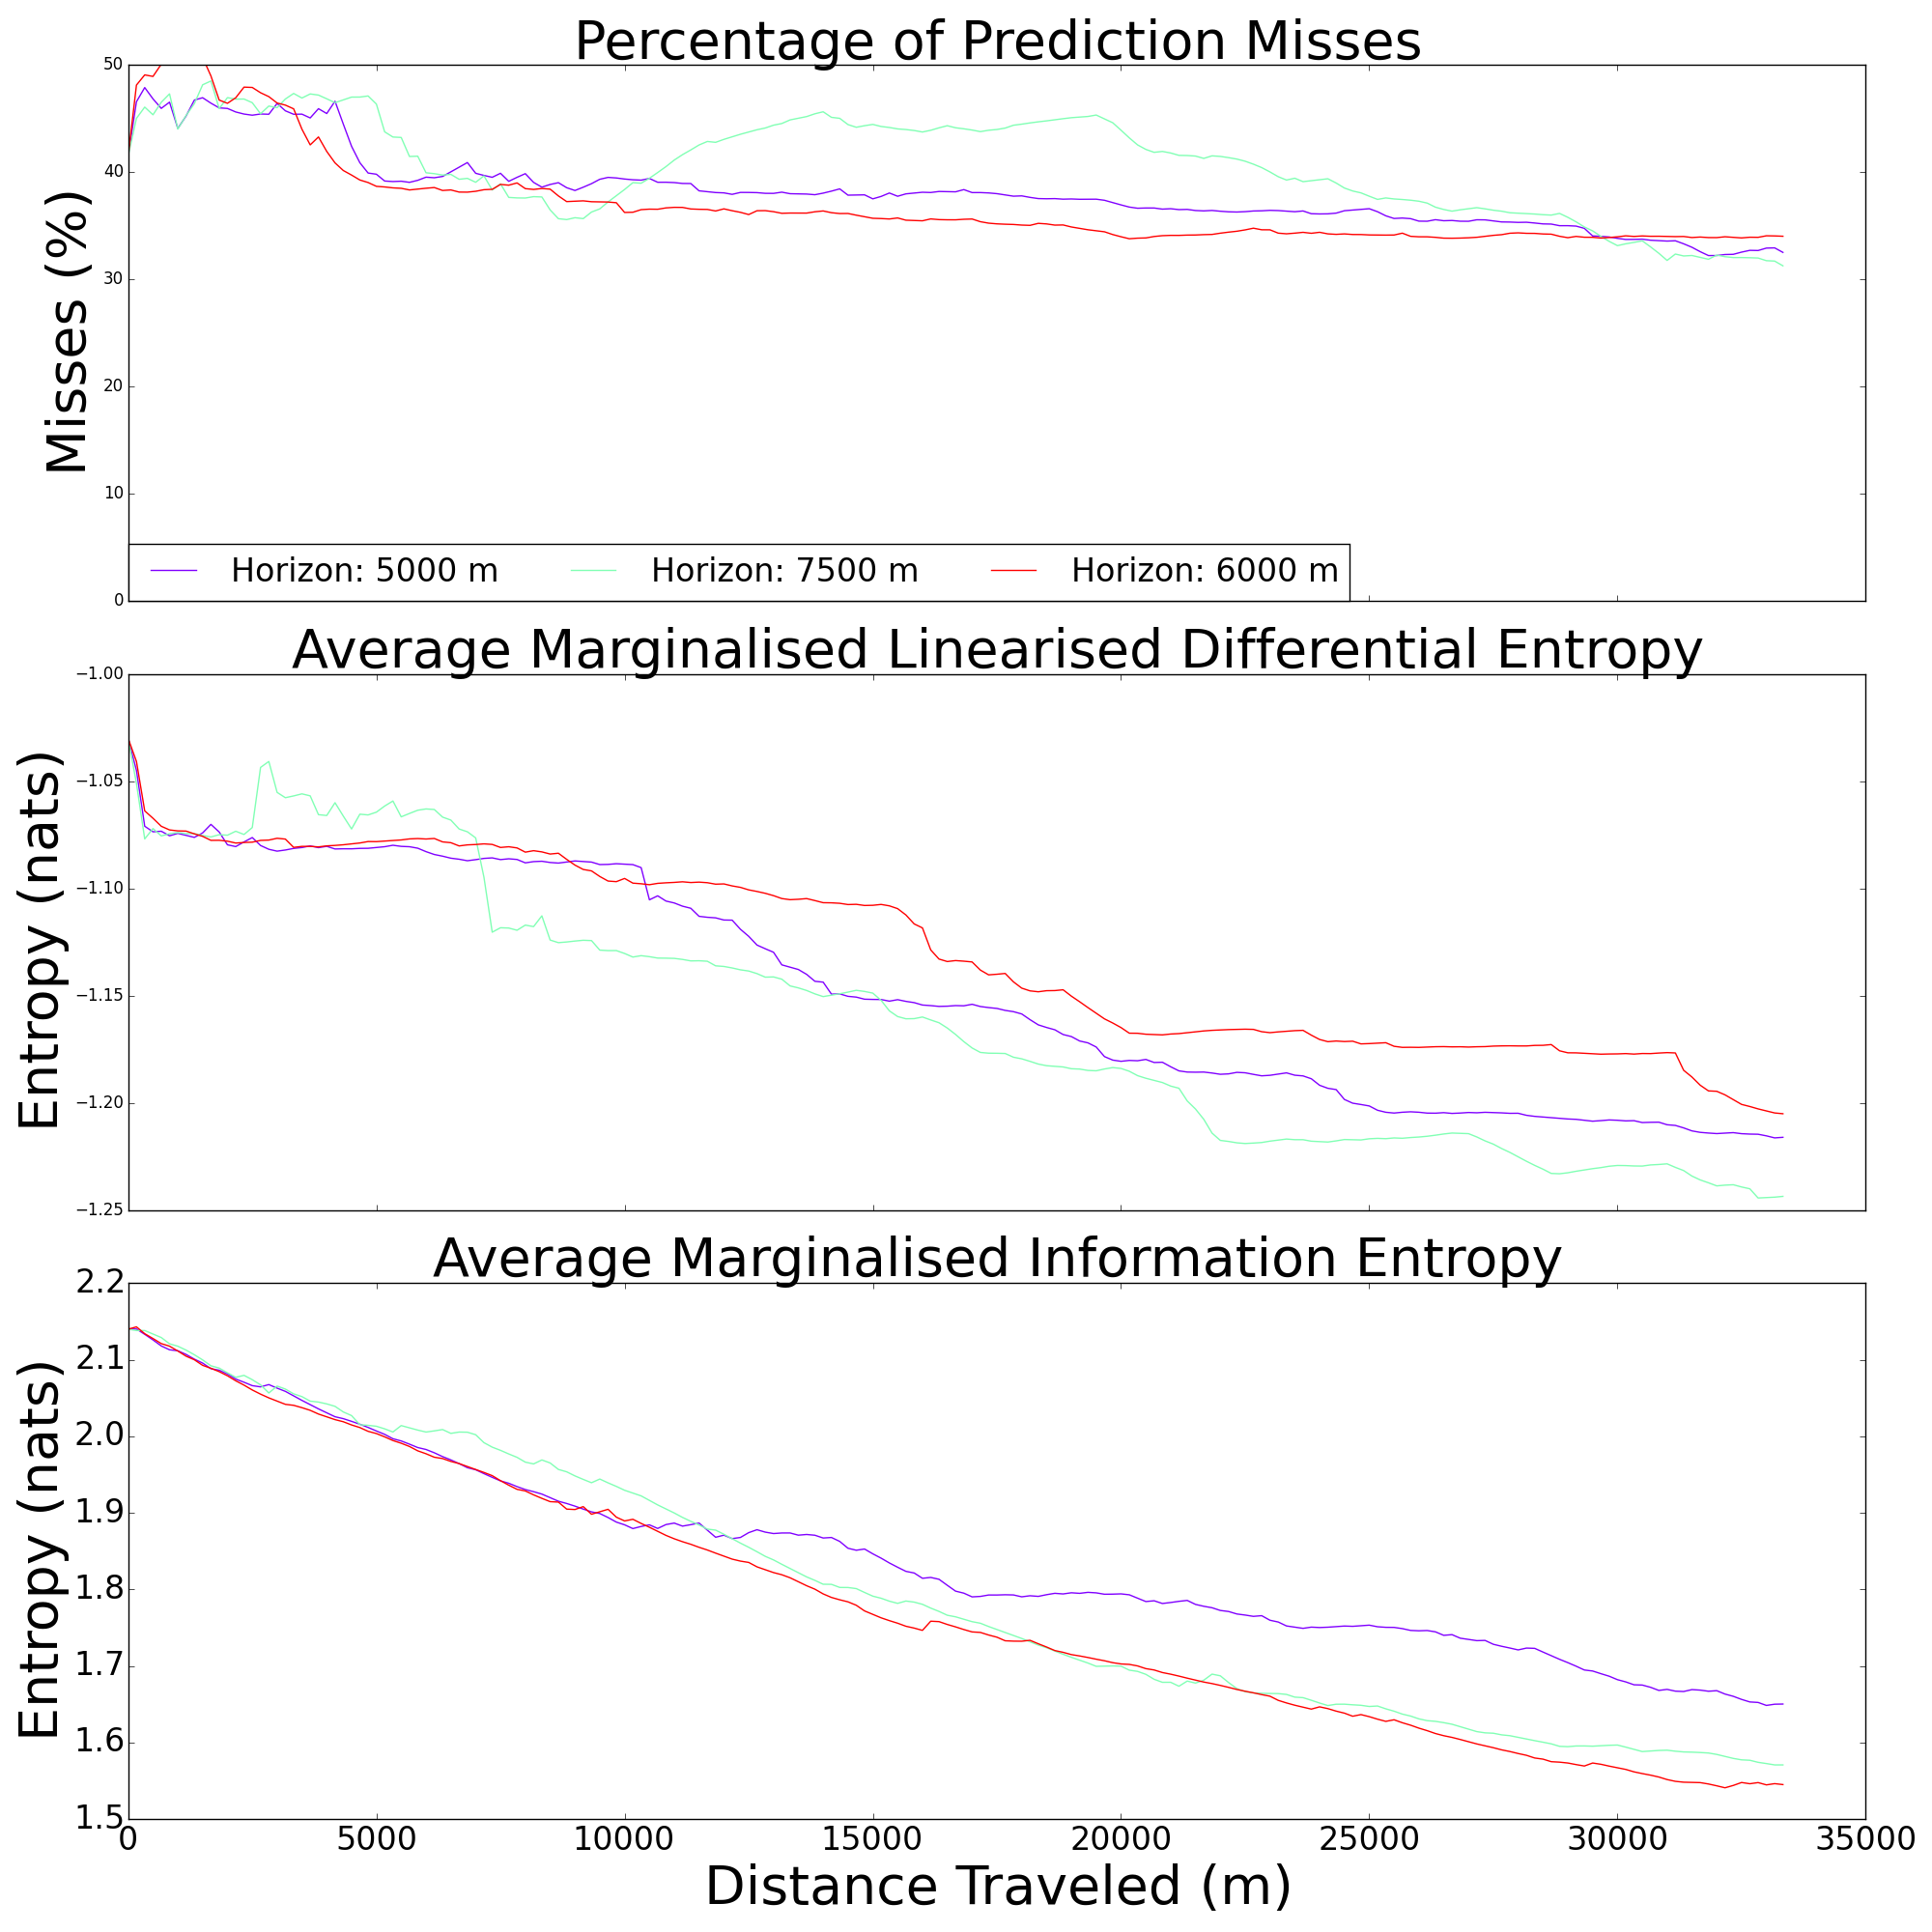
\includegraphics[width = \linewidth]{Figures/compare_horizons.png}
		\caption{Horizon Effects}
		\label{Figure:Results:CompareHorizons}
		\end{figure}
	
		In figures \ref{Figure:Results:CompareHorizons} and \ref{Figure:Results:CompareLocations} we show the stability and consistency of the approach under varying horizon lengths and starting locations for the case of Scott reef.
		
		\begin{figure}[!htbp]
		\centering
			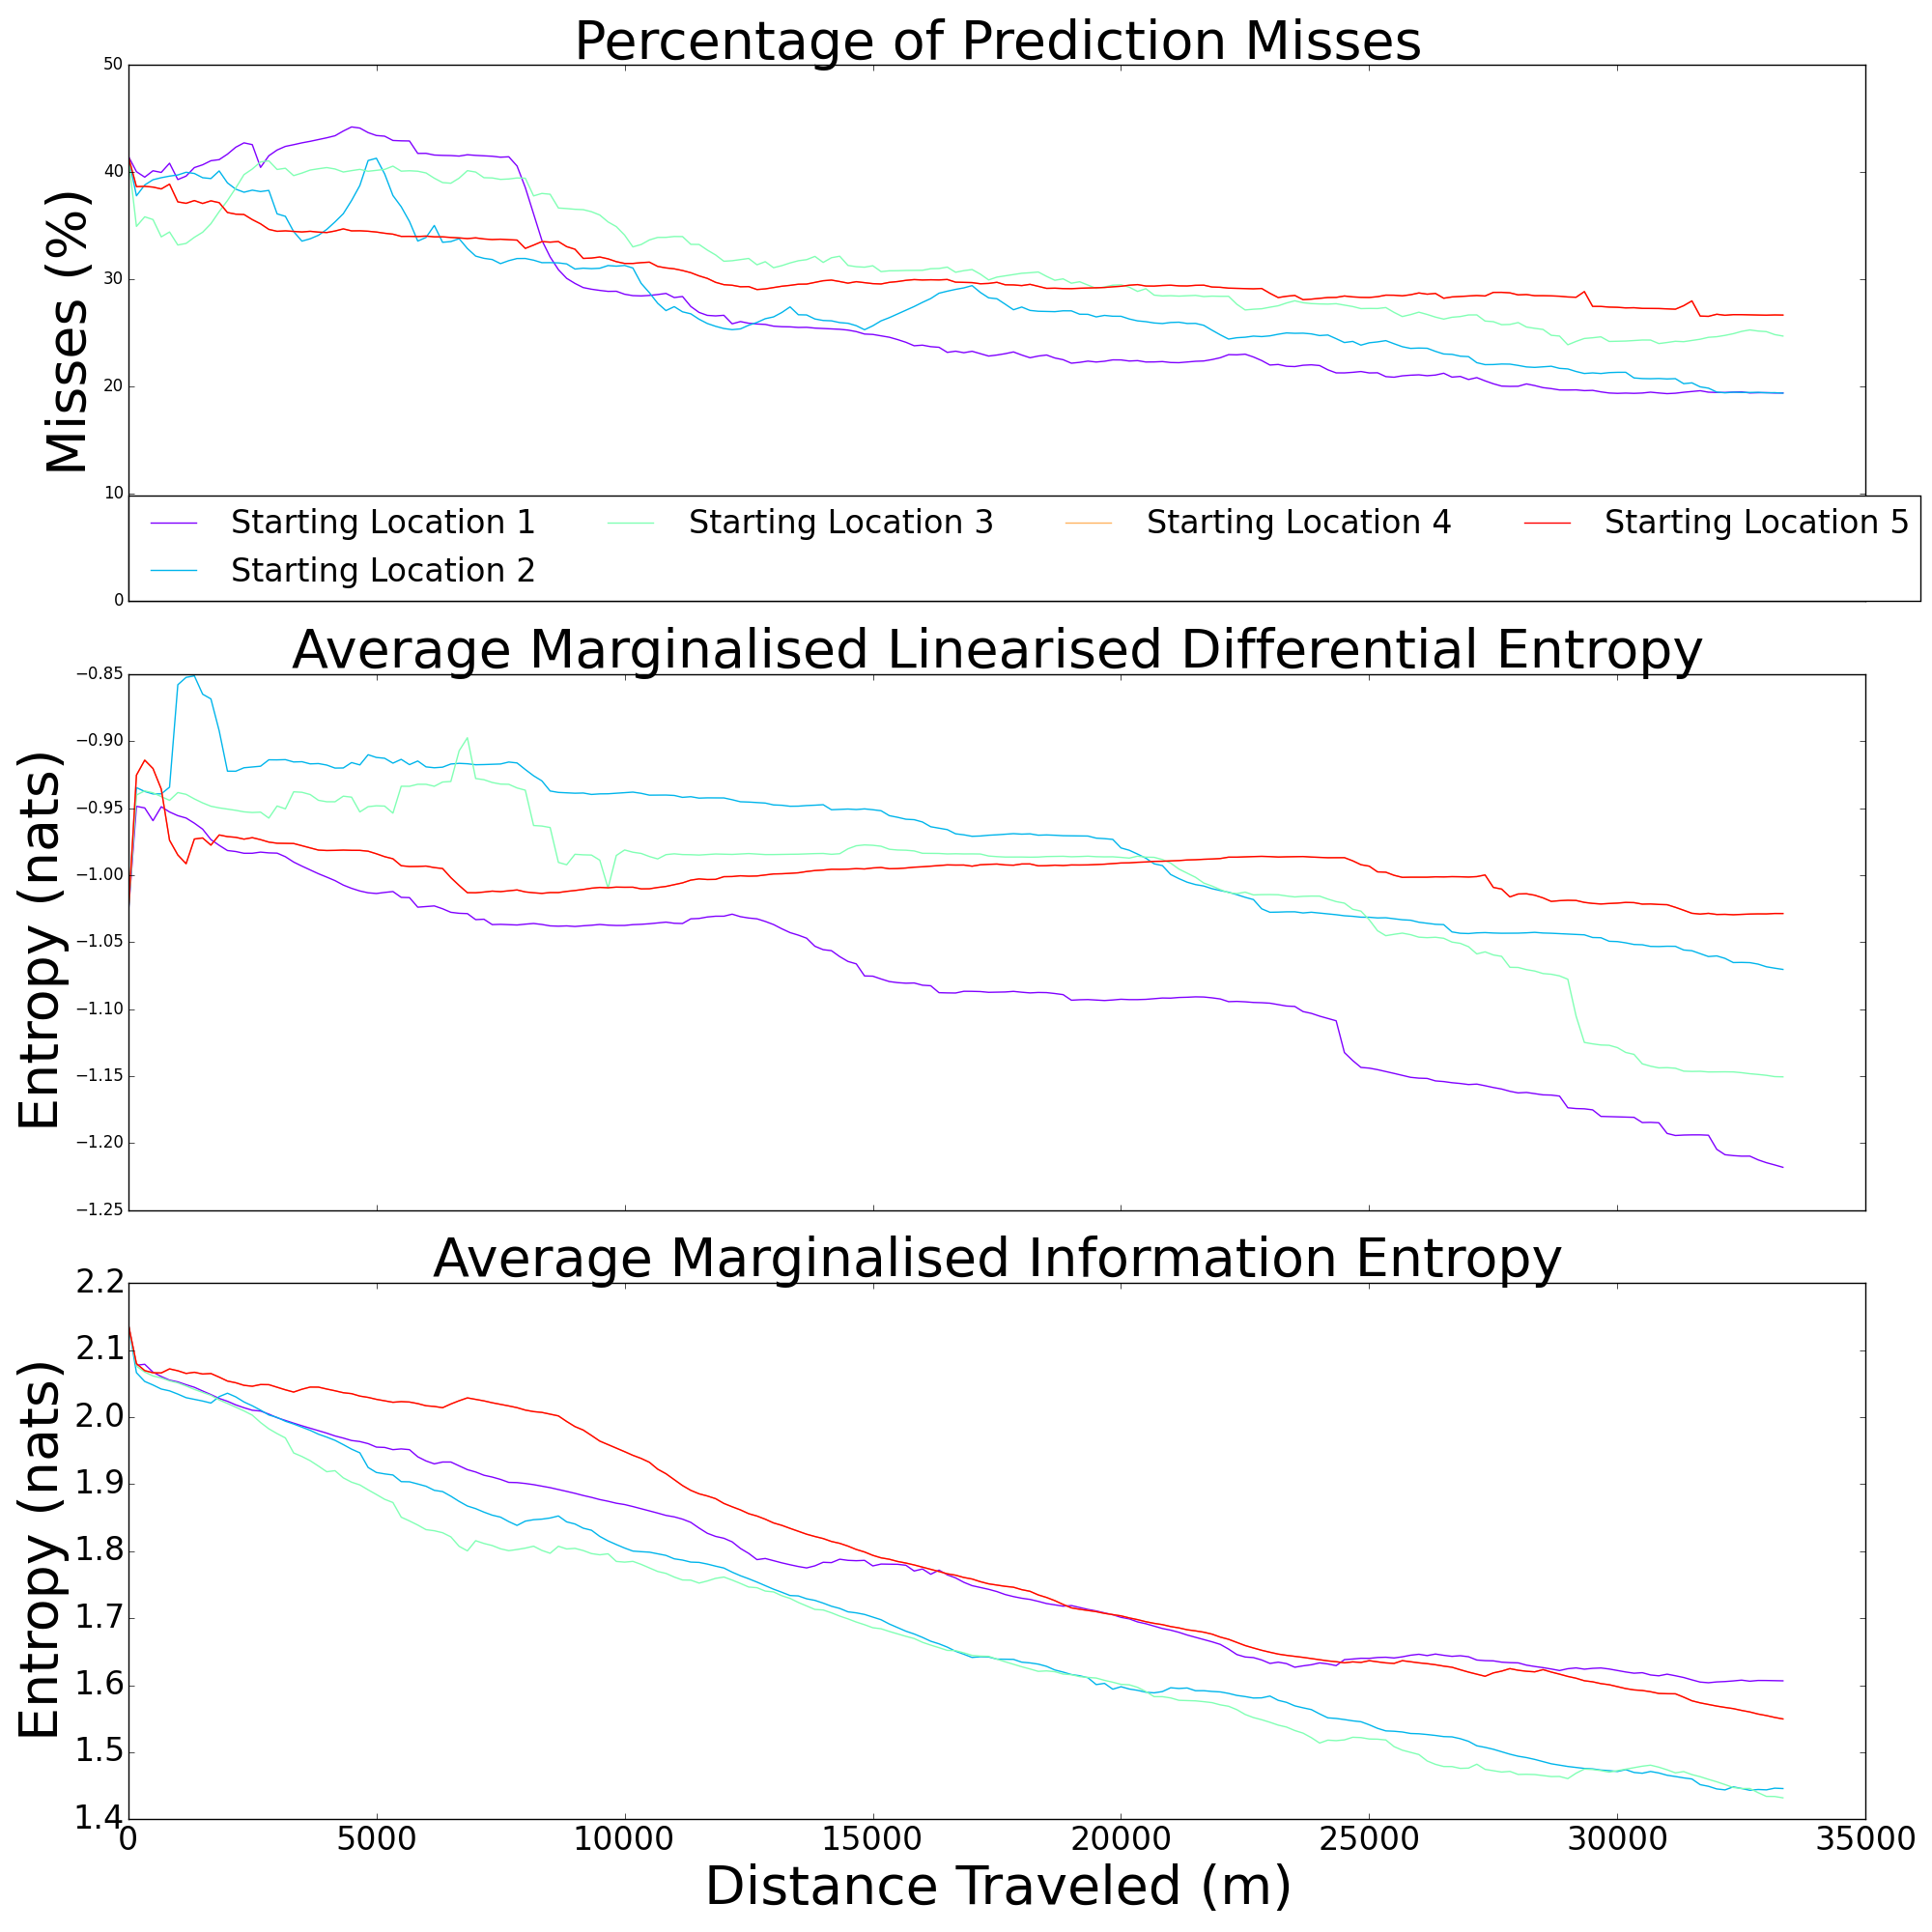
\includegraphics[width = \linewidth]{Figures/compare_locations.png}
		\caption{Horizon Effects}
		\label{Figure:Results:CompareLocations}
		\end{figure}
		
		Figures \ref{Figure:Results:OptimalPathLDE} and \ref{Figure:Results:OptimalPathMCJE} show snapshots of the resulting path under linearised differential entropy and Monte Carlo estimated joint information entropy respectively as the acquisition function. The snapshots are taken at 0 km, 8.3 km, 16.7 km, and 33.3 km into the journey. For each method, three snapshot series are presented, visualising the marginalised prediction information entropy, marginalised linearised differential entropy, and the prediction map. The circle represents the horizon length for which the vehicle considers in at each time step. The vehicle resides at the center of that circle. The path with empty circles represent the path it has taken, and the path with fixed hexagons extending from the current location represent the immediate proposed path from the receding horizon optimisation.
		
		As we expect, the two paths from the two methods are similar, with only minor differences with the linearised differential entropy approach achieving a misclassification ratio of approximately 4\% less. Unlike other methods, both the LDE and MCJIE method take into consideration the mutual information of the proposed path. In the figure shown, the Monte Carlo approach uses 1000 sample draws from the GP classifier to estimate the joint distribution for 30 control points. It is expected that the Monte Carlo approach can perform slightly better, albeit with high computational requirements, if more sample draws are used.
		
		This results demonstrates that under a receding horizon formulation, using linearised differential entropy as the acquisition function achieves lower misclassification rate on average than other acquisition functions - most importantly Monte Carlo estimated joint information entropy.
			
%		From experimental tests:
%			-A larger horizon is not always more beneficial. The entropy of faraway regions that it considers may become meaningless by the time it actually gets there, as the model would have significantly changed. On the other hand, it cannot be too short, or it will suffer the same problem as a greedy approach (not seeing ahead, getting stuck in local regions, not recognising joint information)
%			-For the scott reef data, a good horizon range is 5000.0 m, for horizons more than 6000.0 m the result will hit diminishing returns and may actually hurt the performance. This happens as the model predictions and entropies at far away regions for which it was considering changes too much that during its way there the model has changed too much and it is no longer interested in such regions. This results in fast varying path proposals and may result in instability. It is about balancing obtaining reasonable information in reasonable time against reaching for information that may be outdated by the time it is collecting it.
%			
%		Mention that:
%			-We are demonstrating that in the case of a feature space that does not contain the spatial coordinates for which path planning in based on, the Monte Carlo Joint Information Entropy Method may spent a lot of time in a single region where it is locally rich in span of a subspace of the feature space. However, this is suboptimal as this means it is giving up on trying to go for other regions that may have an even richer span of the feature space. The linearised differential entropy method focuses its efforts (prioritises) the decision boundaries in the feature space at the expense of overlooking regions with less observations. This leads to smoother paths as it will look at all elements of the feature space. As long as one of the features is spatially correlated (depth in our case), this will lead to smoother paths.




%\section{Mapping Benthic Habitats with Gaussian Process Classifiers}
%\label{Section:BenthicMapping}
%
%	\begin{figure*}[!htbp]
%	\centering
%		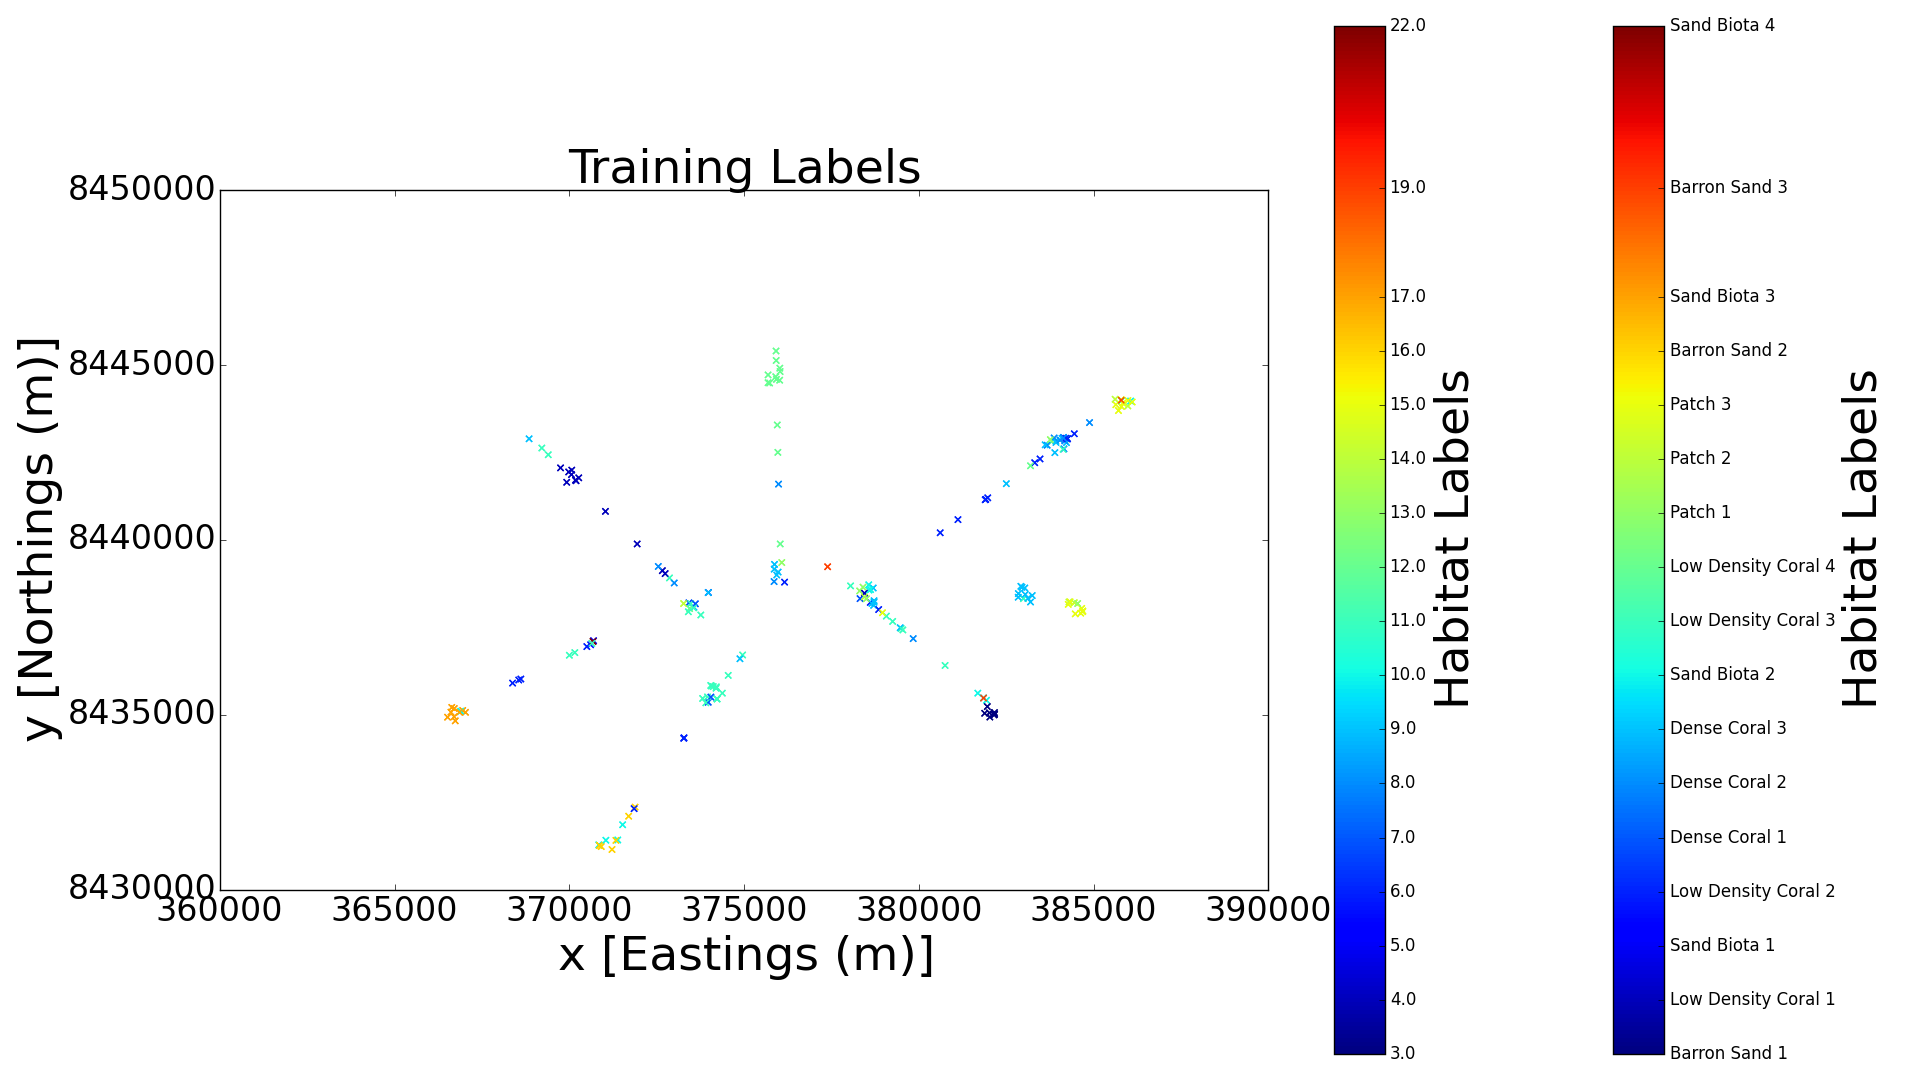
\includegraphics[width = 0.32\linewidth]{Figures/scott_reef_modeling/Figure1.png}
%		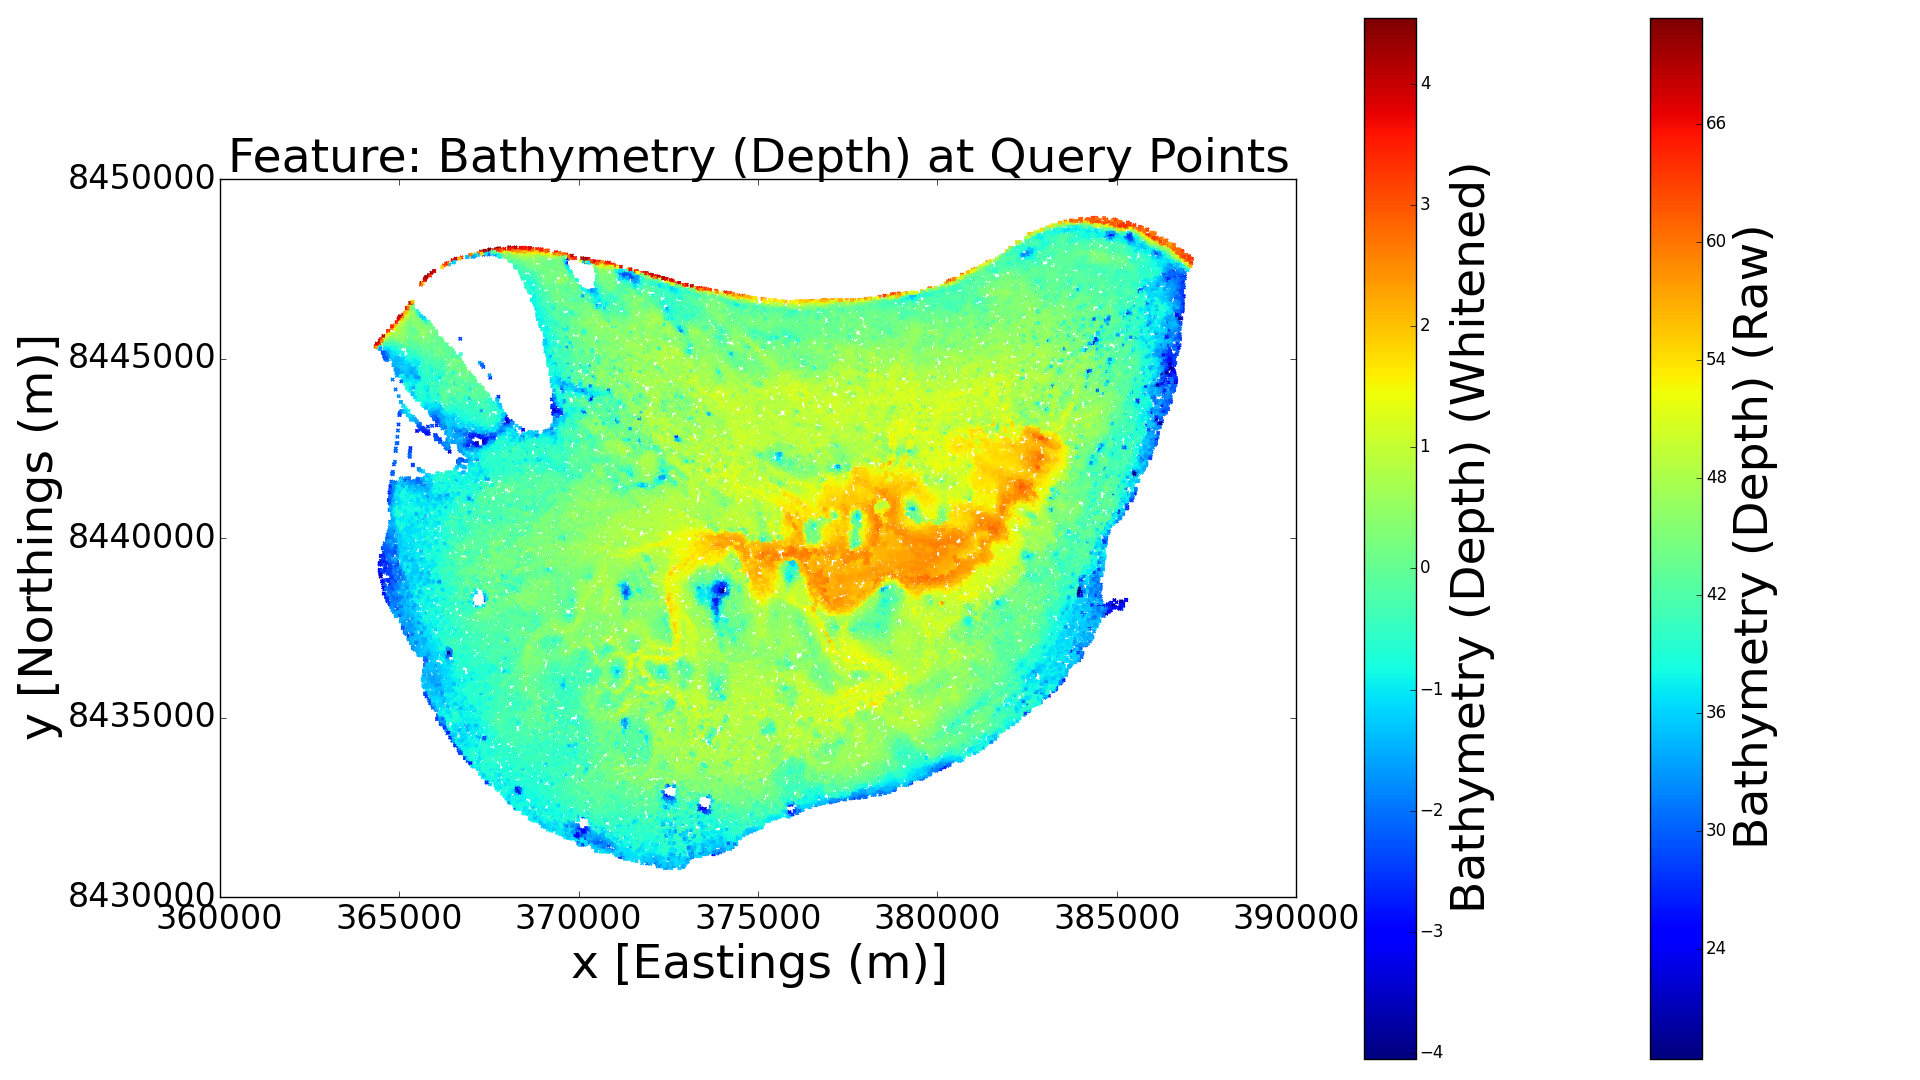
\includegraphics[width = 0.32\linewidth]{Figures/scott_reef_modeling/Figure2.png}
%		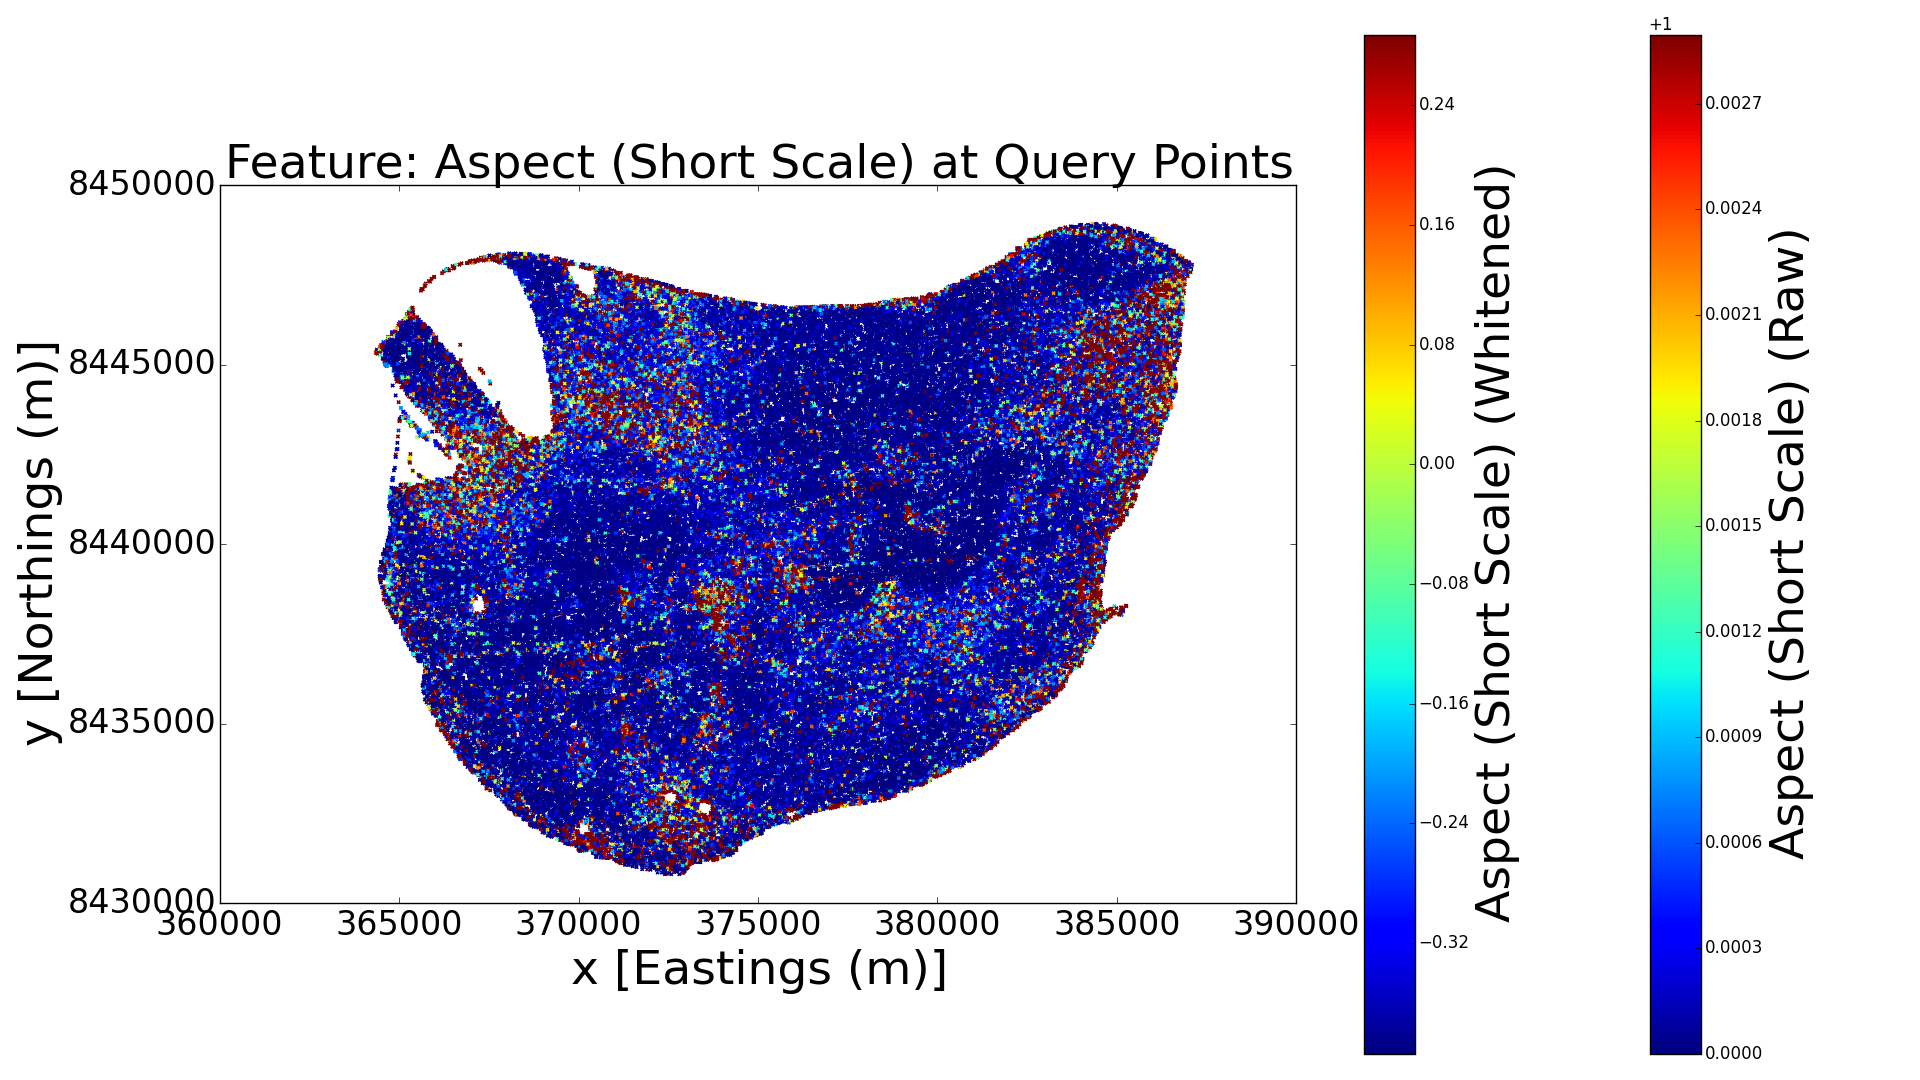
\includegraphics[width = 0.32\linewidth]{Figures/scott_reef_modeling/Figure3.png}
%		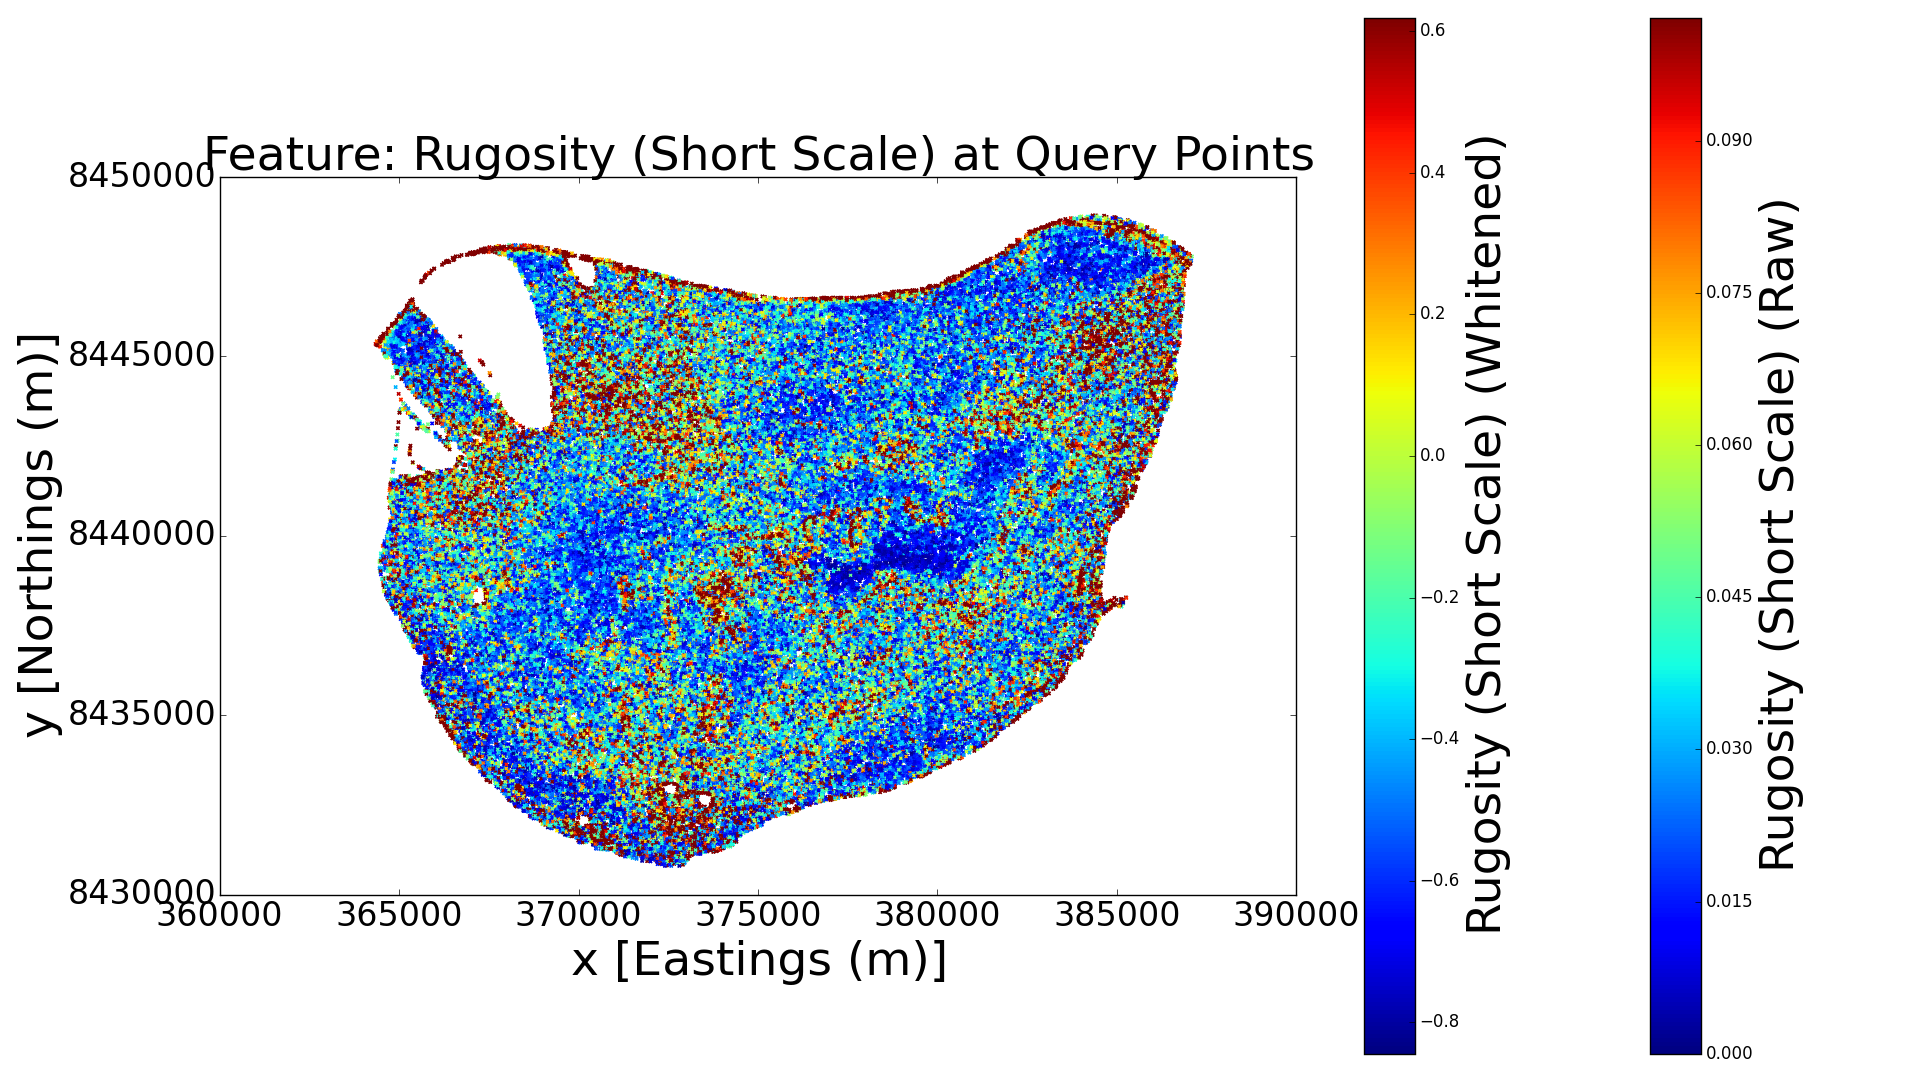
\includegraphics[width = 0.32\linewidth]{Figures/scott_reef_modeling/Figure4.png}
%		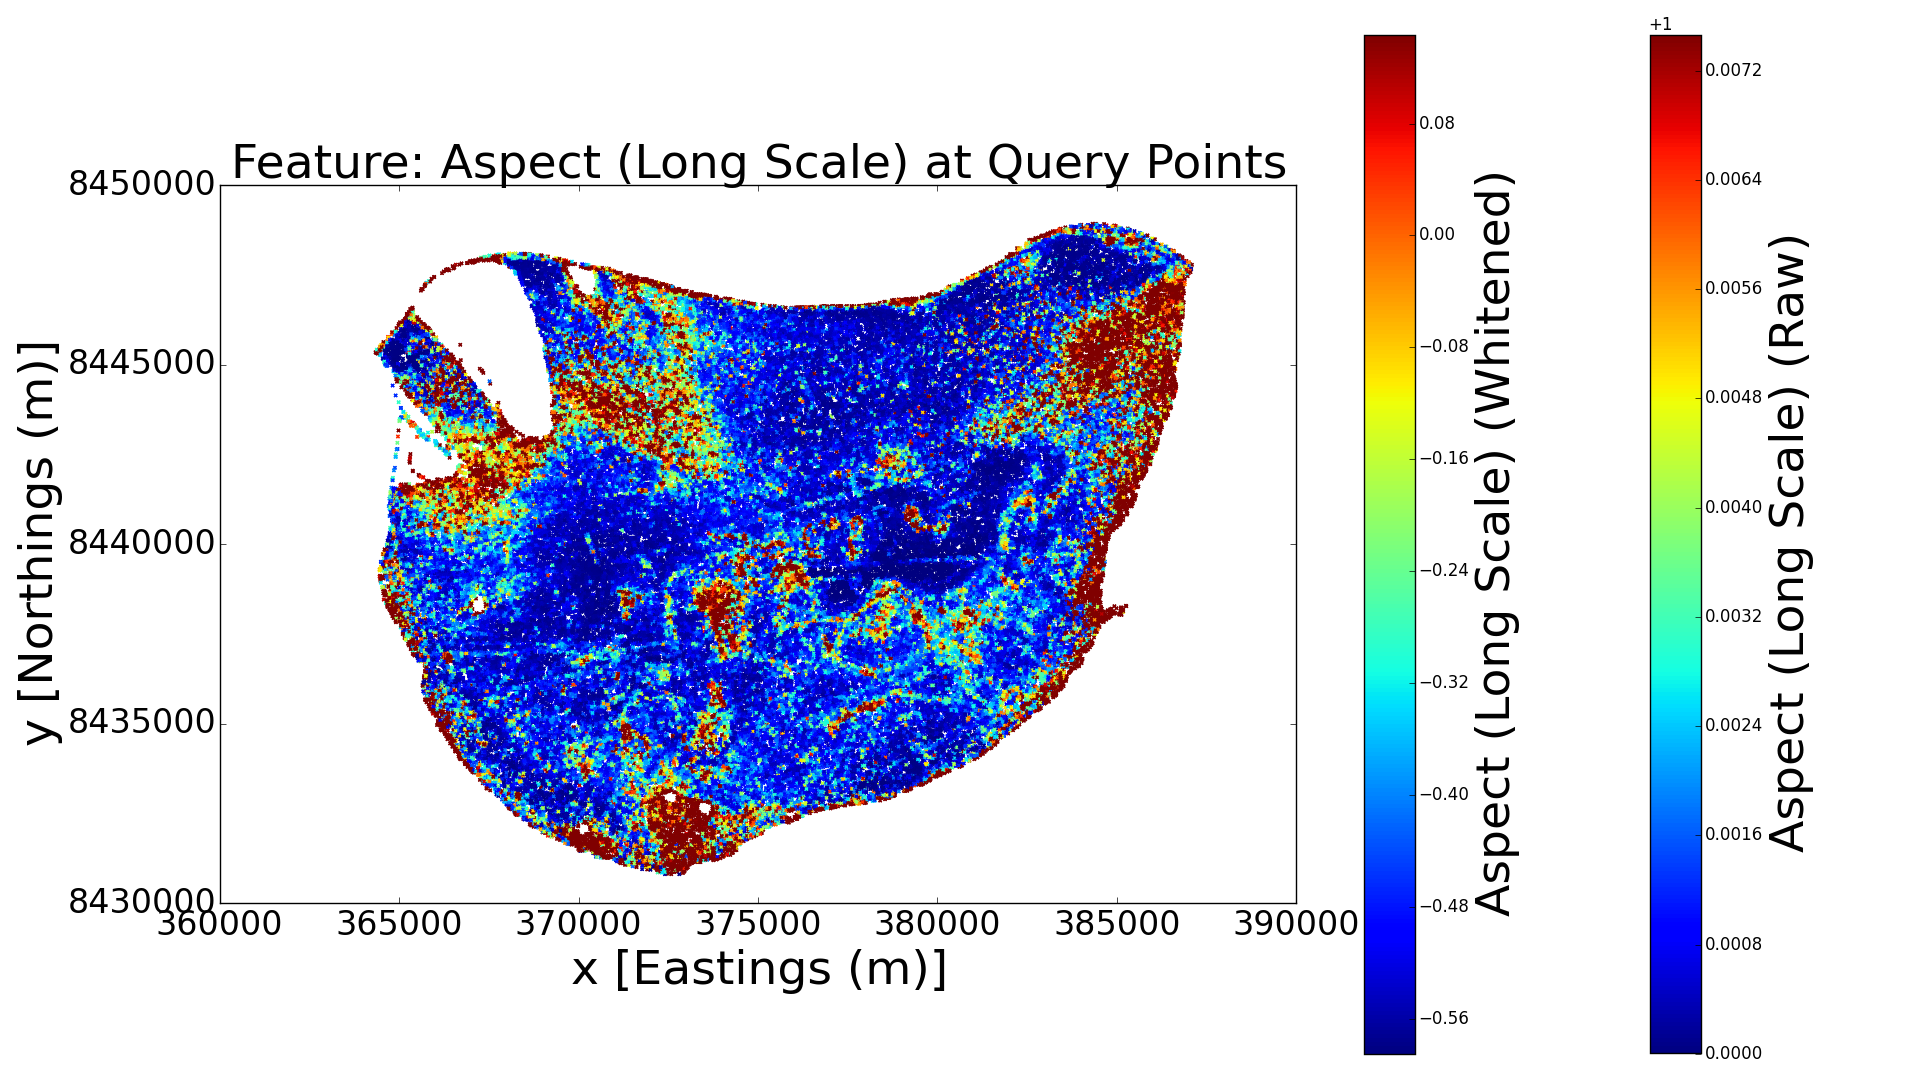
\includegraphics[width = 0.32\linewidth]{Figures/scott_reef_modeling/Figure5.png}
%		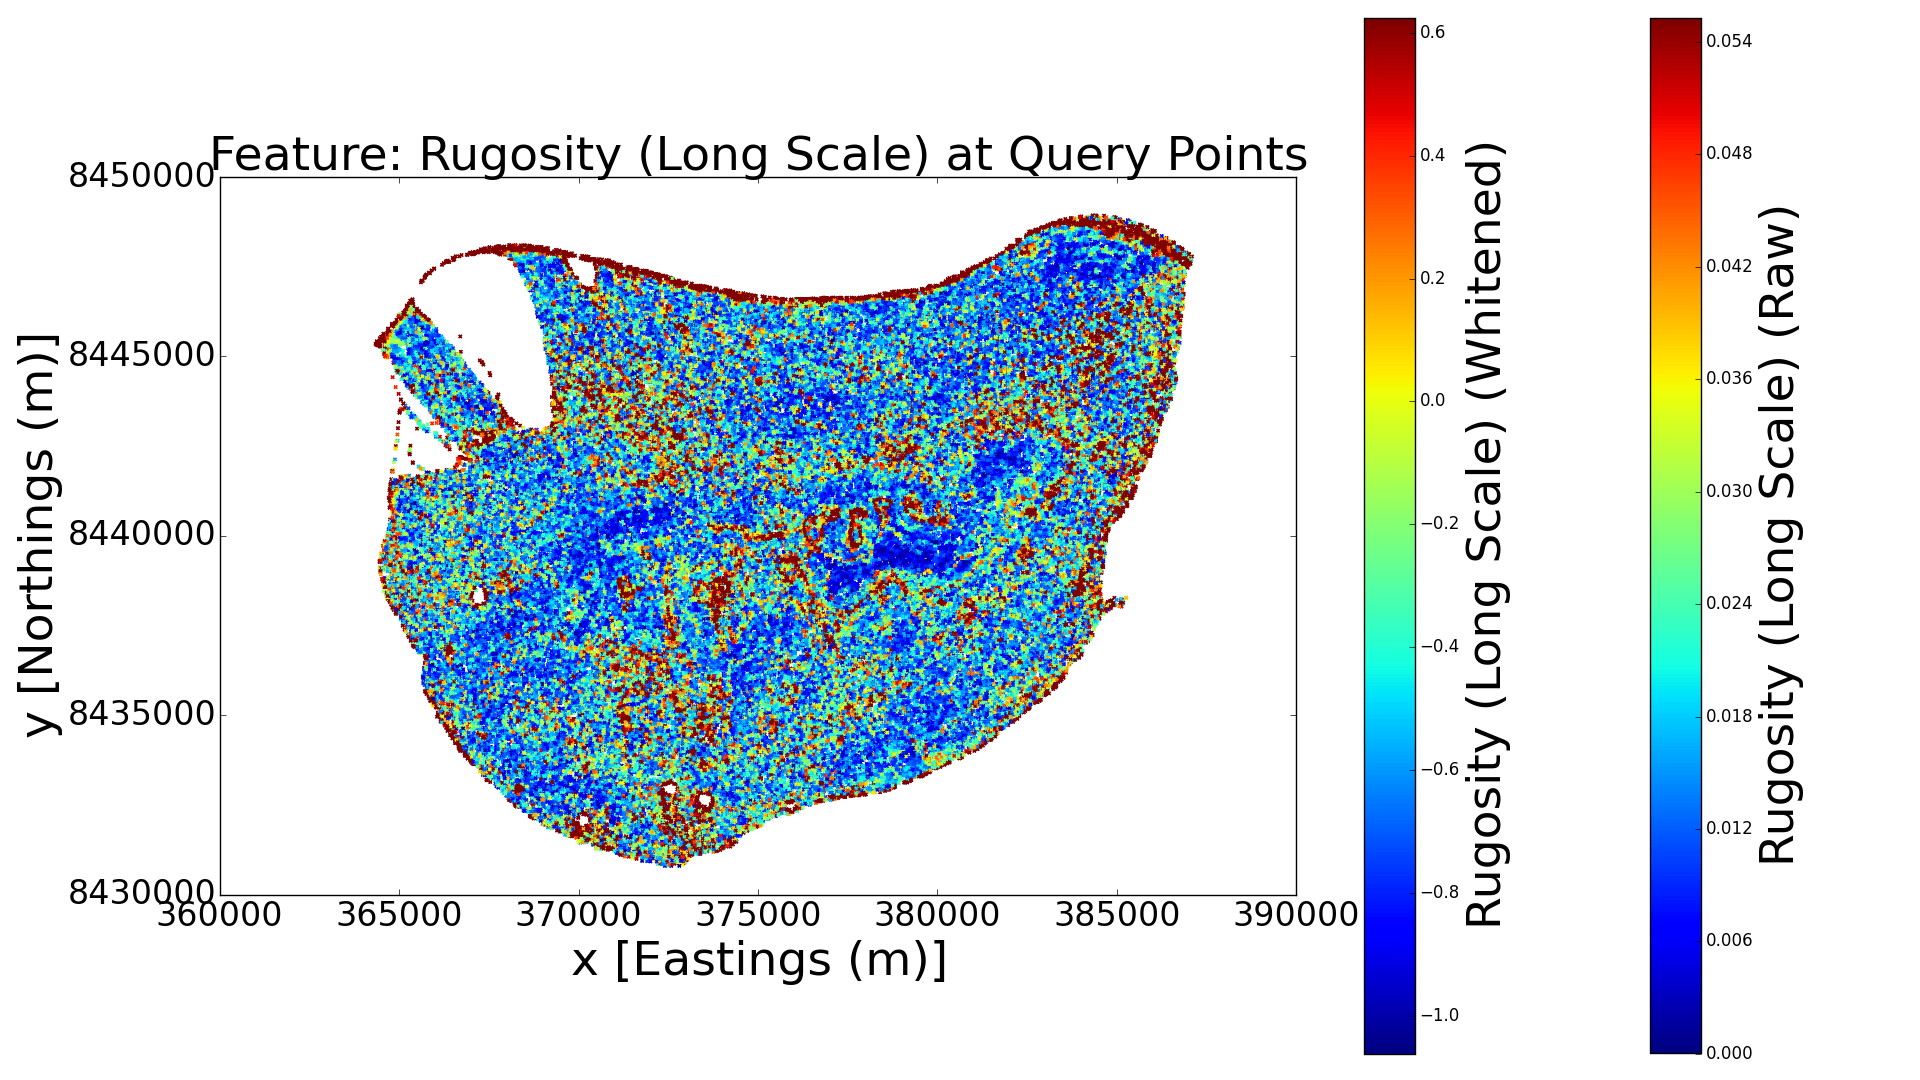
\includegraphics[width = 0.32\linewidth]{Figures/scott_reef_modeling/Figure6.png}
%	\caption{Scott Reef Bathymetric Features}
%	\label{Figure:Results:ScottReefBathymetricFeatures}
%	\end{figure*}
%	
%	In this paper we will focus on applying the modeling and path planning techniques on the datasets collected from past missions at Scott Reefs, Western Australia \cite{ScottReefData}. While the dataset consists of a detailed map of the bathymetric features across the seafloor, the benthic habitats have only been observed through seven linear tracks extending from the middle to the edge of the reef (figure \ref{Figure:Results:ScottReefBathymetricFeatures}). The aim is to distinguish between the 17 different benthic zones and map the benthic habitats of the Scott reef region accurately in the shortest amount of travel time.
%		
%	\subsection{Model Structure and Features}
%		
%		The benthic habitat observations obtained from past mission tracks, together with the bathymetric features observed at those locations, form the training data and labels for the Gaussian process classifier (figure \ref{Figure:Results:ScottReefBathymetricFeatures}). To reduce computational requirements, 200 training points were sampled from those tracks for initial modeling.
%		
%		The Gaussian process classifier is chosen to model the benthic habitats upon five bathymetric features - bathymetric depth, aspect (short scale), rugosity (short scale), aspect (long scale), and rugosity (long scale) (figure \ref{Figure:Results:ScottReefBathymetricFeatures}). The images are built from 10000 query points randomly sampled from the dataset. It is presumed that the nature of the habitat depends on the structure of the seafloor terrain and depth, and that the locations of the habitat itself should have minimal effect. Thus, spatial coordinates are not included in the feature set.
%		
%		To measure the relative performance between modeling and path planning techniques, a synthetic ground truth is generated separately (figure \ref{Figure:Results:ScottReefSyntheticTruth}). Note that this ground truth was generated using a separate sample of the training tracks and does not necessary represent the physical reality at Scott reef.
%	
%		\begin{figure}[!htbp]
%		\centering
%			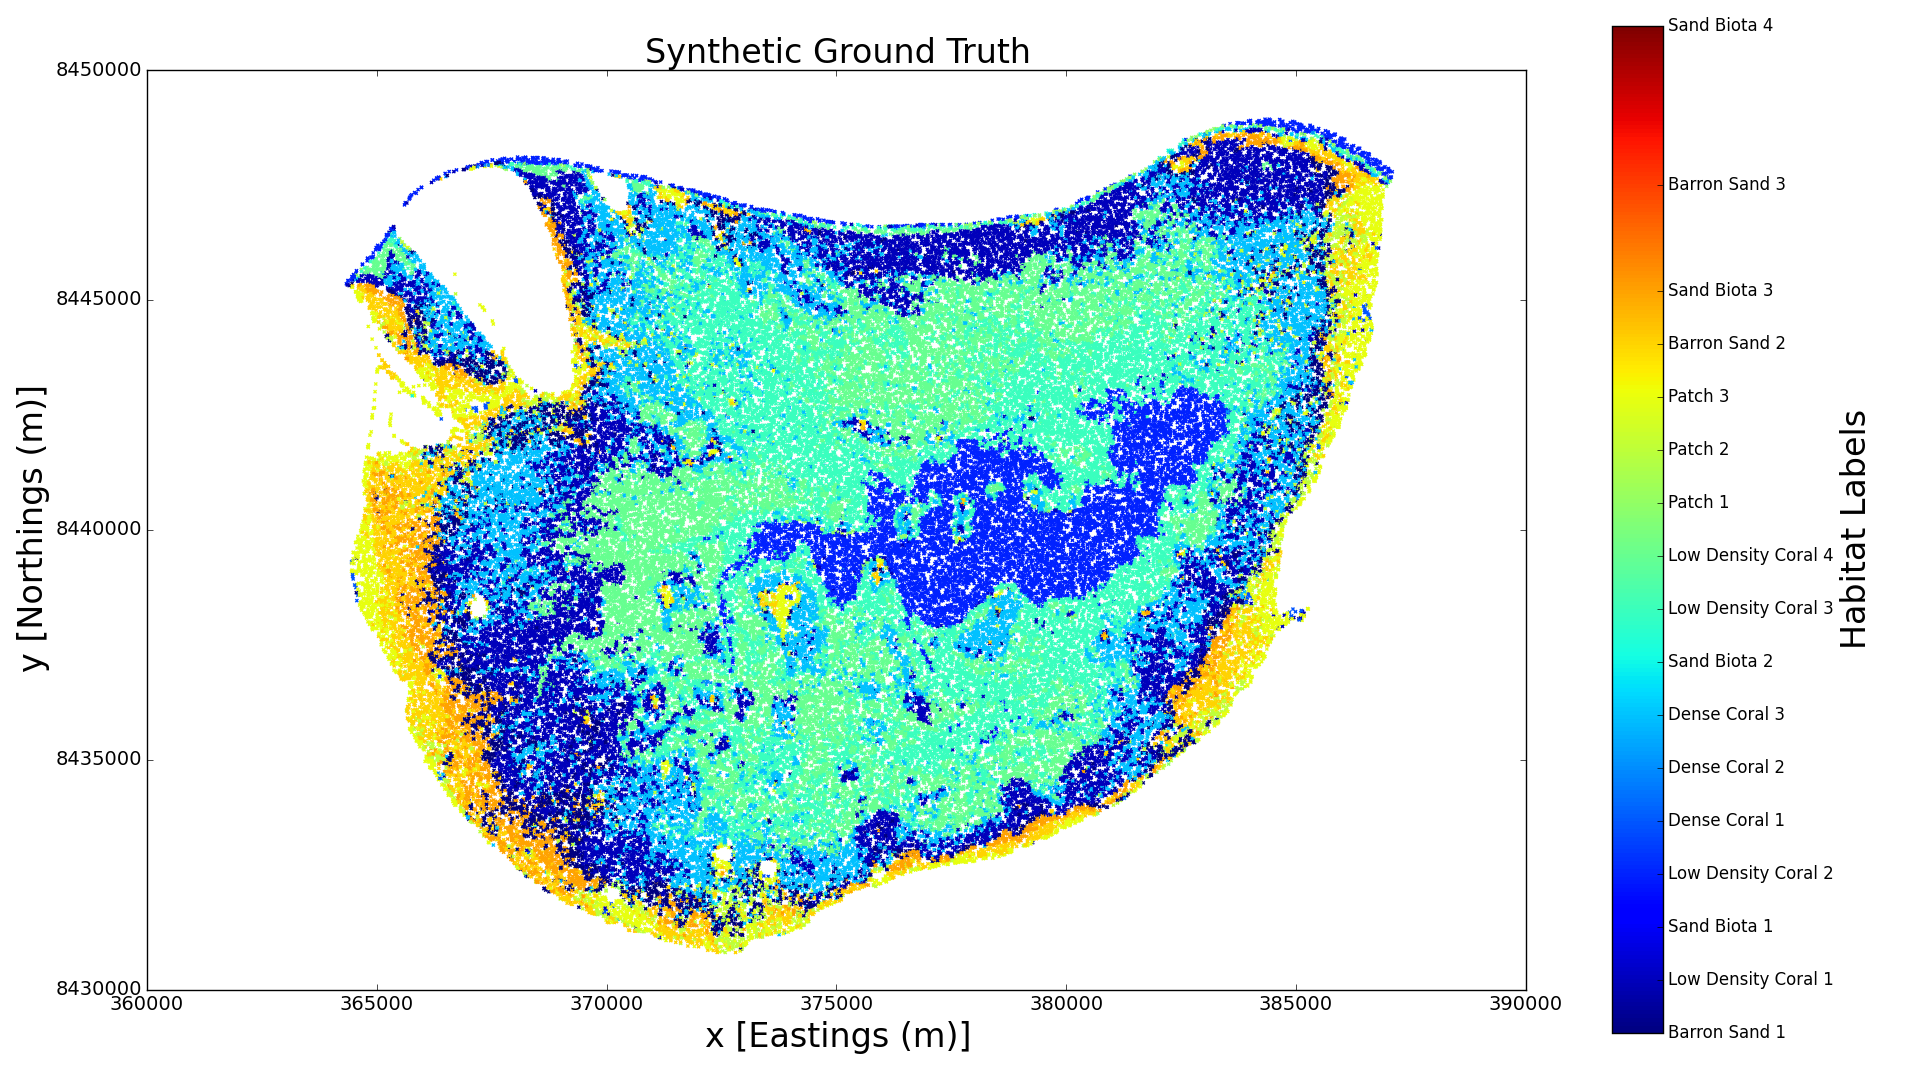
\includegraphics[width = \linewidth]{Figures/scott_reef_modeling/Figure7.png}
%		\caption{Scott Reef: Synthetic Ground Truth}
%		\label{Figure:Results:ScottReefSyntheticTruth}
%		\end{figure}
%		
%	\subsection{Gaussian Processes Classifiers}
%
%		The Scott reef bathymetric-benthic modeling problem is a multiclass classification problem with 17 distinct classes. We perform the modeling using a Gaussian process classifier under Laplace's approximation with a squared exponential (Gaussian) kernel. The likelihood response function employed is the probit response (figure \ref{Figure:LikelihoodResponses}), which provide better linearisation properties discussed in the next section.
%				

					

		


		
		

		

					

	

		
		
\section{Conclusions and Future Work}
\label{Section:Conclusion}

	In this paper we motivate, define, and derive the use of linearised differential entropy as an alternative acquisition function to informative path planning. We demonstrate the use of such an acquisition function under a receding horizon approach, and verify its performance on collected bathymetric and benthic data at Scott Reef. We show that this approach achieves lower misclassification rate on average in comparison to Monte Carlo methods and Greedy methods.
	
	This work is ongoing and more investigation is required to fully understand the properties of the linearised differential entropy measure and its interpretation. As LDE is not an approximation to the usual prediction entropy, theoretical justifications of its use should couple its experimentation justification presented in this paper.
	
	We also plan to test the method more thoroughly with more variations. Specifically, the effects of horizon length, number of control points, and the tolerances of the optimisers used should be rigorously investigated. 
	
\section*{Acknowledgments}

	This work is supported by the Australian Centre of Field Robotics, the University of Sydney, and National ICT Australia (NICTA).
	
%% This section was initially prepared using BibTeX.  The .bbl file was
%% placed here later
%\bibliography{publications}
%\bibliographystyle{named}
%% The file named.bst is a bibliography style file for BibTeX 0.99c

\bibliographystyle{named}
\bibliography{acra2015}

\end{document}

